\documentclass[main.tex]{subfiles}
\newsavebox\Axis
\newsavebox\Axisb
\newcommand\chapterlabel{electrons}
\setcounter{figurenewcounter}{0}


\begin{document}
\linenumbers

  

\chapter[Electronic structure of atoms]{Electronic structure of atoms}
%\label{ch:atoms}


   
         \begin{marginfigure}
      \begin{tikzpicture} \node (a) at (0,0) {\includegraphics[width=4cm]{chapter3/figure1}} node[rotate=90, font=\tiny] at ([yshift=.5cm,xshift=.1cm]a.south east) {\textsuperscript{\textcopyright} PngImg} ;
\end{tikzpicture}
\end{marginfigure}


\lettrine[lines=4]{\color{black!45}M}{atter} is everywhere around you, from the water you drink to the air you inhale. Matter is made of elements and elements are made of atoms. In the world we can also find light, that somehow at first sight seems different than matter. Light is warm and it has color. This chapter covers the structure of the atoms, with a focus on the structure of the many electrons than atoms are made of. It also focuses on light and the interaction of light with matter. You will be able to understand differences in electronic configuration.
 
\begin{marginfigure}%LEARNING GOALS BOX
\begin{mytcbox}{GOALS}
\begin{enumerate}[label=\protect\circled{\color{white}\arabic*}]
\item Compute frequency, wavelength and the energy of light
\item Compute Hydrogen energy levels  
\item Compute Hydrogen transition energies 
\item Obtain electronic configurations
\item Compare periodic properties
\end{enumerate}
\end{mytcbox}
\vspace{1cm}
\begin{tcolorbox}[enhanced,colback=red!5!white,colframe=black!50!red,boxrule=1pt,
  arc=0pt,outer arc=0pt,drop heavy lifted shadow]
\faGears\ 
\docenvdef{Discussion:} Look around your apartment and find four different types of radiation.\end{tcolorbox}
\vspace{1cm}
    \begin{shadequote}[l]{Schr\"{o}dinger}
The present is the only things that has no end.\end{shadequote}   
 \end{marginfigure}%LEARNING GOALS BOX

 

\section{The nature of light}
Light--also called electromagnetic radiation--is a form or energy. When talking about light we normally refer to visible radiation. However, there are many different types of radiation. Think about the light coming from a bulb, or the radiation that warms up your food in a microwave, or even when you warm up a pizza in the over. This section will cover the properties of light.

\sloppy
\begin{description}
\item[\docfilehook{Light as a wave}{}]
Light behaves as a wave. Waves are characterized by their frequency, wavelength and amplitude. The wavelength of a wave ($\lambda$, lambda) is the distance between identical points on successive waves (or successive peaks). The frequency of a wave ($\nu$, nu) is the number of waves that pass through a particular point in one second. The amplitude ($A$) of a wave is the vertical distance from the zero to the top of the peak, of from the zero to the bottom of the peak. The amplitude of a wave its related to the intensity of the radiation. The speed of light through the vacuum is $3\times 10^{8}$m/s. However, the speed of light depends on the medium and light tends to slow down when traveling in a medium different than vacuum. 

\stepcounter{figurenewcounter}   \refstepcounter{figure}  \label{Fig:{\chapterlabel}\thefigurenewcounter}
     \begin{center}\begin{tikzpicture}[xscale=1,yscale=1, every node/.style={scale=0.9}]
            \begin{scope}[xshift =-25em, yshift =0em, scale=1]
  \draw[->] (0,0) -- (0,1.3);
  \draw[->] (0,0)--(4.3,0) node[font=\large,black, below, pos = 1.1] {\small time};
  \draw[domain=0:4,samples=100,blue] plot(\x,{sin(\x r*10)});

\draw[<->] (0.8,1.2) -- node[above]{\small $\nu$} (1.4,1.2);
  \draw[dashed] (0.8,0) -- (0.8,1.3);
  \draw[dashed] (1.4,0) -- (1.4,1.3);
%  \draw[<->] (pi/2,1.15) -- node[above]{\small $\nu$} (pi/2+1.28,1.15);
   \end{scope} 
       \begin{scope}[xshift =-10em, yshift =0em, scale=1]
  \draw[->] (0,0) -- (0,1.3);
  \draw[->] (0,0)--(4.3,0) node[font=\large,black, below, pos = 1.1] {\small space};
  \draw[domain=0:4,samples=100,red] plot(\x,{sin(\x r*4)});
  \draw[dashed] (pi/2+0.4,0) -- (pi/2+0.4,1.3);
  \draw[dashed] (pi/2+0.65+1.3,0) -- (pi/2+0.65+1.3,1.3);
  \draw[<->] (pi/2+0.4,1.15) -- node[above]{\small $\lambda$} (pi/2+0.65+1.28,1.15);
    \draw[<->] (0.4,0) -- node[above, rotate=0, xshift=-0.4em, yshift=-0.9em ]{\small $A$} (0.4,1);
       \end{scope} 
        \begin{scope}[xshift =0em, yshift =0em]
\node[text width=14cm, fontscale=0.1] at (-8em,-5em) { \begin{bf}\color{black}\bfseries\large Figure \ref{Fig:{\chapterlabel}\thefigurenewcounter} \end{bf} Properties of waves. Waves are characterized by its frequency, wavelength and amplitude and in the vacuum they travel at the speed of light.   };
   \end{scope} 
\end{tikzpicture}\end{center}



\item[\docfilehook{Frequency and energy}{Frequency and energy}] Light travels in time. That is the reason you can hear a whistle from afar. The \emph{frequency} of a radiation--the frequency of a specific type of light--characterizes how this radiation oscillates in time. The unit of frequency is the hertz and frequency is represented by the symbol $\nu$. At the same time, frequency is connected to the energy of radiation. High frequency radiation are very energetic. Think for example of gamma rays; these type of radiation produced in nuclear plant has very high frequency and hence is very energetic. The formula that related frequency with energy is:%\resizeableyellownote{2.5}{1}{Add this formula to your flashcard.}
\begin{equation*}
\boxed{  E=h\nu  } \quad \textcolor{blue}{\text{Frequency formula}}
\end{equation*}
where:
\begin{where}
 \item $E$   is the energy in joules
  \item $h=6.6\times 10^{-34}$ is called Plank's constant 
 \item $\nu$  is frequency in hertz (Hz=$s^{-1}$)
\end{where}
As you can see in the previous formula, the frequency is directly proportional to frequency.
This equation has a historical character and was stablished by Max Plank in 1900.
When a solid is warmed up to temperatures beyond 800K--this is called a black body--it emits radiation of different color. The radiation emitted changes as the body is heated, and the light emitted goes from red to white. In the later part of the nineteenth century, experiments found that the amount of energy produced by a black body depends on the wavelength of the emitted radiation. However, none of the current theories (thermodynamics and classical physics) were able to explain that phenomena. Plank came with a solution for the dilemma. Classical physics assumes that radiant energy is a continuos and radiation can be emitted and absorbed at any amount. In order to explain the blackbody radiation, Plank suggested that there is a minimum package of energy so that radiation could only be exchanges in discrete packages. The smallest amount of energy that can be emitted in the form of electromagnetic radiation was called \emph{quamtum} and equals to $h\nu$, with $h$ being Plank's constant. Based on his theory, the energy emitted by light can only be whole-number multiples of $h\nu$. This hypothesis was the key to solve the blackbody radiation dilemma and change physics forever, marking the beginning of a new quantum theory.

\item[\docfilehook{The speed of light}{}] 
All light travel at the same speed in the vacuum and this speed is called the speed of light, $c$. The numerical value of the speed of light is 299 792 458 m / s which is close to $3\times 10^8$ m/s. When light travels in a medium, like water of glass, its velocity can be lower than the speed of light as the medium slows down the propagation of light. At the same time, the speed of light is used to related two properties of light: the frequency and its wavelength:
\begin{equation*}
\boxed{  c=\nu\cdot \lambda  } \quad \textcolor{blue}{\text{the speed of light}}
\end{equation*}
where:
\begin{where}
 \item $c$   is the speed of light in the vacuum, $3\times 10^8$ m/s
 \item $\lambda$  is wavelength in $m$
  \item $\nu$  is the frequency in Hz.
\end{where}


If we want $\lambda$ to be in nm we can use the following formula:
%\resizeableyellownote{2.5}{1}{Add this formula to your flashcard.}
\begin{equation*}
\boxed{  \nu=\frac{3\times 10^{17}}{\lambda}  } 
\end{equation*}
where:
\begin{where}
 \item $\nu$   is frequency in Hz
 \item $\lambda$  is wavelength in $nm$
  \item $3\times 10^{17}=c\cdot 10^{9}$   was adjusted to be able to use $\lambda$ in nm

\end{where}
Mind that all radiation always travels at the speed of light. At the same time, this speed is the maximum speed allowed for any object, based on the principles of relativity.



\item[\docfilehook{Wavelength and energy}{Wavelength and energy}] Light also travels in space. As it moves, it oscillates in space. Think about dropping a stone into a lake. As you drop the pebble, the energy from the pebble propagates in the surface in water. The energy of light also propagates in space and the \emph{wavelength} of a radiation is the distance between two consecutive peaks. As such, wavelength, represented by the letter $\lambda$ and with units of $nm$ is also related to energy by means of the formula:
%\resizeableyellownote{2.5}{1}{Add this formula to your flashcard.}
\begin{equation*}
\boxed{  E=\frac{1.98\times 10^{-16}}{\lambda}  } \quad \textcolor{blue}{\text{wavelength formula}}
\end{equation*}
where:
\begin{where}
 \item $E$   is the energy in joules
 \item $\lambda$  is wavelength in $nm$
  \item $1.98\times 10^{-16}=h\cdot c\cdot 10^{9}$  was adjusted to be able to use $\lambda$ in nm
\end{where}
Mind that wavelength is inversely related to energy. That means, the larger wavelength the smaller energy. Also mind that wavelength refers to the movement of light in space and frequency refers to the movement in time. 






%\begin{marginfigure}[0cm]
%      \includegraphics{chapter3/figure1-1}
%      \caption{White light contains many colors.}
%      \label{fig:marginfig2}
%   \end{marginfigure}
%   
%   
%   \begin{marginfigure}[0cm]
%     \begin{tikzpicture}[xscale=1,yscale=1]
%  \draw[->] (0,0) -- (0,1.3);
%  \draw[->] (0,0)--(4.3,0) node[font=\large,black, below, pos = 1.1] {seconds};
%  \draw[domain=0:4,samples=100,blue] plot(\x,{sin(\x r*5)});
%  \draw[dashed] (pi/2,0) -- (pi/2,1.3);
%  \draw[dashed] (pi/2+1.3,0) -- (pi/2+1.3,1.3);
%  \draw[<->] (pi/2,1.15) -- node[above]{\small $\nu$} (pi/2+1.28,1.15);
%\end{tikzpicture}
%      \caption{Frequency refers to time}
%   \end{marginfigure}
%   
%   
%      \begin{marginfigure}[0cm]
%     \begin{tikzpicture}[xscale=1,yscale=1]
%  \draw[->] (0,0) -- (0,1.3);
%  \draw[->] (0,0)--(4.3,0) node[font=\large,black, below, pos = 1.1] {nm};
%  \draw[domain=0:4,samples=100,red] plot(\x,{sin(\x r*4)});
%  \draw[dashed] (pi/2+0.4,0) -- (pi/2+0.4,1.3);
%  \draw[dashed] (pi/2+0.65+1.3,0) -- (pi/2+0.65+1.3,1.3);
%  \draw[<->] (pi/2+0.4,1.15) -- node[above]{\small $\lambda$} (pi/2+0.65+1.28,1.15);
%\end{tikzpicture}
%      \caption{Wavelength refers to space}
%   \end{marginfigure}
   
   
   
   
\begin{example} %%%%%%%%%%%%%%%%%%%%%%%% EXAMPLE BOX
Calculate: (a) the energy of a radiation with wavelength of 300nm; (b) the energy of a radiation with frequency of $10^{19}$ Hz; (c) the frequency of a radiation with wavelength of 300nm.\\
\textlcsc{ \textcolor{dgreen}{\Large \textbf{Solution}} }\\
(a) To answer the first question we will use the wavelength formula, as wavelength is given ($\lambda=300nm$) and we need to calculate the energy ($E$), in Joules:
\begin{equation*}
E=\frac{1.98\times 10^{-16}}{\lambda}=\frac{1.98\times 10^{-16}}{300}=6.6\times 10^{-19}J
\end{equation*}
(b) To answer the second question we will use the frequency formula, as frequency is given ($\nu=10^{19}Hz$) and we need to calculate the energy ($E$), in Joules:
\begin{equation*}
E=6.6\times 10^{-34}\nu=6.6\times 10^{-34}\cdot 10^{19}=6.6\times 10^{-15}J
\end{equation*}
(c) To answer the last question we will use the formula that related frequency with wavelength--through the speed of light--as frequency is asked and wavelength is given ($\lambda=300nm$); mind the units of frequency are herts:
\begin{equation*}
\nu=\frac{3\times 10^{17}}{\lambda}=  \frac{3\times 10^{17}}{300}=1\times 10^{15}Hz
\end{equation*}
\faDiamond\ \textlcsc{ \textcolor{dgreen}{\Large \textbf{Study Check}} }\\
Calculate: (a) the wavelength of radiation with energy of $5.6\times 10^{-19}J$; (b) the frequency of a radiation with frequency of $4.8\times 10^{-18}J$; (c) the wavelength of a radiation with frequency of $2\times 10^{15}Hz$.
\flushright Answer: (a) $353nm$; (b) $7.2\times 10^{10}Hz$; (c) $4.1\times 10^{6}nm$
\end{example}%%%%%%%%%%%%%%%%%%%%%%%% EXAMPLE BOX


%\newpage

\item[\docfilehook{The electromagnetic spectrum of light}{}] 
Visible light consist of electromagnetic waves, which have an electric field and magnetic field component. These two components share the same wavelength, frequency, and speed but are perpendicular to each other.
 %%%%%%%%%%%FIGURE %%%%%%%%%%%
 \vspace{-1cm}\stepcounter{figurenewcounter}   \refstepcounter{figure}  \label{Fig:{\chapterlabel}\thefigurenewcounter}\begin{center}
  \begin{tikzpicture} [every node/.style={scale=0.9}]
          \begin{scope}[xshift =0em, yshift =5em]% Axes
    \draw (-1,0,0) node[above] {$x$} -- (5,0,0);
    \draw (0,0,0) -- (0,2,0) node[above] {$y$};
    \draw (0,0,0) -- (0,0,2) node[left] {$z$};
    % Propagation
    \draw[->,ultra thick] (5,0,0) -- node[above] {$c$} (6,0,0);
    % Waves
    \draw[thick] plot[domain=0:4.5,samples=200] (\x,{cos(deg(pi*\x))},0);
    \draw[gray,thick] plot[domain=0:4.5,samples=200] (\x,0,{cos(deg(pi*\x))});
    % Arrows
    \foreach \x in {0.1,0.3,...,4.4} {
      \draw[->,help lines] (\x,0,0) -- (\x,{cos(deg(pi*\x))},0);
      \draw[->,help lines] (\x,0,0) -- (\x,0,{cos(deg(pi*\x))});
    }
    % Labels
    \node[above right] at (0,1,0) {$\bm{E}$};
    \node[below] at (0,0,1) {$\bm{B}$};
      \end{scope} 
            \begin{scope}[xshift =-2em, yshift =10em]
\node[text width=5cm, fontscale=0.1] at (-8em,-5em) { \begin{bf}\color{black}\bfseries\large Figure \ref{Fig:{\chapterlabel}\thefigurenewcounter} \end{bf} The electric ($E$) and magnetic ($B$) field components of an electromagnetic wave. Both fields are perpendicular.   };
   \end{scope} 
  \end{tikzpicture}\end{center} 
 %%%%%%%%%%%FIGURE %%%%%%%%%%%

\item[\docfilehook{The double-slit experiment: light diffraction}{}] 
The double-slit experiment was intended to demonstrate the wave nature of light. When a source of light passes through a narrow opening called slit a bright spot is generates on the other side of the slit. When a source of light passes through two slits surprising results arise. 






%%%%%%%%%%%FIGURE %%%%%%%%%%%
 \stepcounter{figurenewcounter}   \refstepcounter{figure}  \label{Fig:{\chapterlabel}\thefigurenewcounter}\begin{center}
  \begin{tikzpicture} [every node/.style={scale=0.9}, every node/.append style={transform shape}]
                    \begin{scope}[xshift =-40em, yshift =0em]
          \foreach \x in {-0.5,-0.25,0} {
            \draw (\x,-1) -- (\x,1);
        }
        \foreach \x in {-0.375,-0.125,-0.125} {
            \draw[dashed] (\x,-1) -- (\x,1);
        }
        \draw[fill=black!10] (0.5,-2,-1) -- (0.5,-2,1) -- (0.5,2,1) -- (0.5,2,-1) -- (0.5,-2,-1);
        \fill (0.5,0,0) circle (0.05);
        \foreach \r in {0.25,0.5,...,1.75} {
            \draw (0.5,0) ++(-60:\r) arc (-60:60:\r);
        }
        \foreach \r in {0.125,0.375,...,1.875} {
            \draw[dashed] (0.5,0) ++(-60:\r) arc (-60:60:\r);
        }
        \draw[fill=black!10] (2,-2,-1) -- (2,-2,1) -- (2,2,1) -- (2,2,-1) -- (2,-2,-1);
        \fill (2,0.5) circle (0.05) (2,-0.5) circle (0.05);
        \foreach \r in {0.25,0.5,...,2} {
            \draw (2,0.5) ++(-60:\r) arc (-60:60:\r);
            \draw (2,-0.5) ++(-60:\r) arc (-60:60:\r);
        }
        \foreach \r in {0.125,0.375,...,2.125} {
            \draw[dashed] (2,0.5) ++(-60:\r) arc (-60:60:\r);
            \draw[dashed] (2,-0.5) ++(-60:\r) arc (-60:60:\r);
        }
        \draw (2,0.5,0.625) -- (2,0.5,0.5);
        \draw (2,-0.5,0.625) -- (2,-0.5,0.5);
        \draw (2,0.5,0.5) -- (2,-0.5,0.5);
        \draw[densely dotted] (2,0.5,0.5) -- (2,0.5,0);
        \draw[densely dotted] (2,-0.5,0.5) -- (2,-0.5,0);
        \draw[fill=black!10] (4,-2,-1) -- (4,-2,1) -- (4,2,1) -- (4,2,-1) -- (4,-2,-1);
        %       LABELLING
        \begin{scope}[canvas is yz plane at x=2,rotate=-90]
            \node[above] at (0,0.5) {S${}_1$};
            \node[below] at (0,-0.5) {S${}_2$};
            \node[left] at (-0.5,0) {d};
        \end{scope}
        \begin{scope}[canvas is yz plane at x=0.5,rotate=-90]
            \node[below left=-0.1cm] at (0,0) {S${}_0$};
        \end{scope}
        \begin{scope}[xshift=4cm,yshift=2cm,rotate=-90,canvas is xy plane at z=0]
            \fill[white] (0,0) rectangle (4,1);
            \begin{axis}[
                width=5.575cm,
                xmin=-0.62,
                xmax=0.62,
                ymin=0,
                ticks=none
            ]
                \addplot [samples=500,black,smooth
                ]
                    {(cos(deg(5*pi*sin(deg(x)))))^(2)*((sin(deg(4*pi*sin(deg(x)))))/(4*pi*sin(deg(x))))^(2)};
                \draw[thin, densely dashed,blue] (axis cs:0.1593,0.1327) -- (axis cs:0.1593,0);
                \draw[thin, densely dashed,blue] (axis cs:-0.1593,0.1327) -- (axis cs:-0.1593,0);
                \draw[thin, densely dashed,blue] (axis cs:0.3941,0.03938) -- (axis cs:0.3941,0);
                \draw[thin, densely dashed,blue] (axis cs:-0.3941,0.03938) -- (axis cs:-0.3941,0);
            \end{axis}
        \end{scope}
        \draw[thin,densely dashed,blue] (2,0) -- (6.9,0);
        \begin{scope}
            \clip (2,-2) rectangle (4,2);
            \draw[thin,densely dashed,blue] (2,0) --    +(15:4);
            \draw[thin,densely dashed,blue] (2,0) --    +(-15:4);
            \draw[thin,densely dashed,blue] (2,0) --    +(32:4);
            \draw[thin,densely dashed,blue] (2,0) --    +(-32:4);
            \draw[thin,densely dashed,red] (2,0) --     +(8:4);
            \draw[thin,densely dashed,red] (2,0) --     +(-8:4);
            \draw[thin,densely dashed,red] (2,0) --     +(24:4);    
            \draw[thin,densely dashed,red] (2,0) --     +(-24:4);               
        \end{scope}
                    \begin{scope}[xshift =30em, yshift =0em]
                \node [rotate=90 ] (a) at (0,0) {\includegraphics[width=5cm]{chapter3/figure1-9}} node[rotate=90, font=\tiny] at ([yshift=-10em,xshift=.1cm]a.south east) {\textsuperscript{\textcopyright} wikipedia} ;
  \end{scope}
              \end{scope}
            \begin{scope}[xshift =-15em, yshift =-5em]
\node[text width=14cm, fontscale=0.1] at (-8em,-5em) { \begin{bf}\color{black}\bfseries\large Figure \ref{Fig:{\chapterlabel}\thefigurenewcounter} \end{bf} The double-slit experiment demonstrating the wave nature of light. Using one slit leads to a single bright spot. Using two slits leads to a set of patterns of light and darkness resulting from the interference of light. Red lines represent destructive interference whereas blue lines represent constructive interferences.   };
   \end{scope} 
  \end{tikzpicture}\end{center} 
 %%%%%%%%%%%FIGURE %%%%%%%%%%%
One would expect to see two bright spots, one per each slit. However, what you really would see would be a series of bright spots and dark spots, resulting of the interference of light. As light is a wave it can interfere and light plus light does not always gives more light, and can sometimes genera darkness. The bright spots result from the constructive interference of the light waves whereas the dark spots result from the destructive interference. Overall, waves propagate energy and the results of the propagation can be more light of less light depending on how these waves interfere.\\
%%%%%%%%%%%%%%%%%%%%%%%%%%%%%%%%%%
 \vspace{1cm}\hspace{-5cm}\begin{minipage}[b]{1.5\linewidth}

	  \begin{tikzpicture} \node (a) at (0,0) {\includegraphics[width=4.5cm, height=4.5cm]{chapter3/figure1-17}} node[rotate=90, font=\tiny] at ([yshift=.5cm,xshift=.1cm]a.south east) {\textsuperscript{\textcopyright} wikipedia} ;
\node[text width=5cm, fontscale=.1] at ([yshift=0.5cm]a.north) {\mytriangle{red}{\small Standing waves of a guitar}};
 
 \node (b) at (6cm,0) {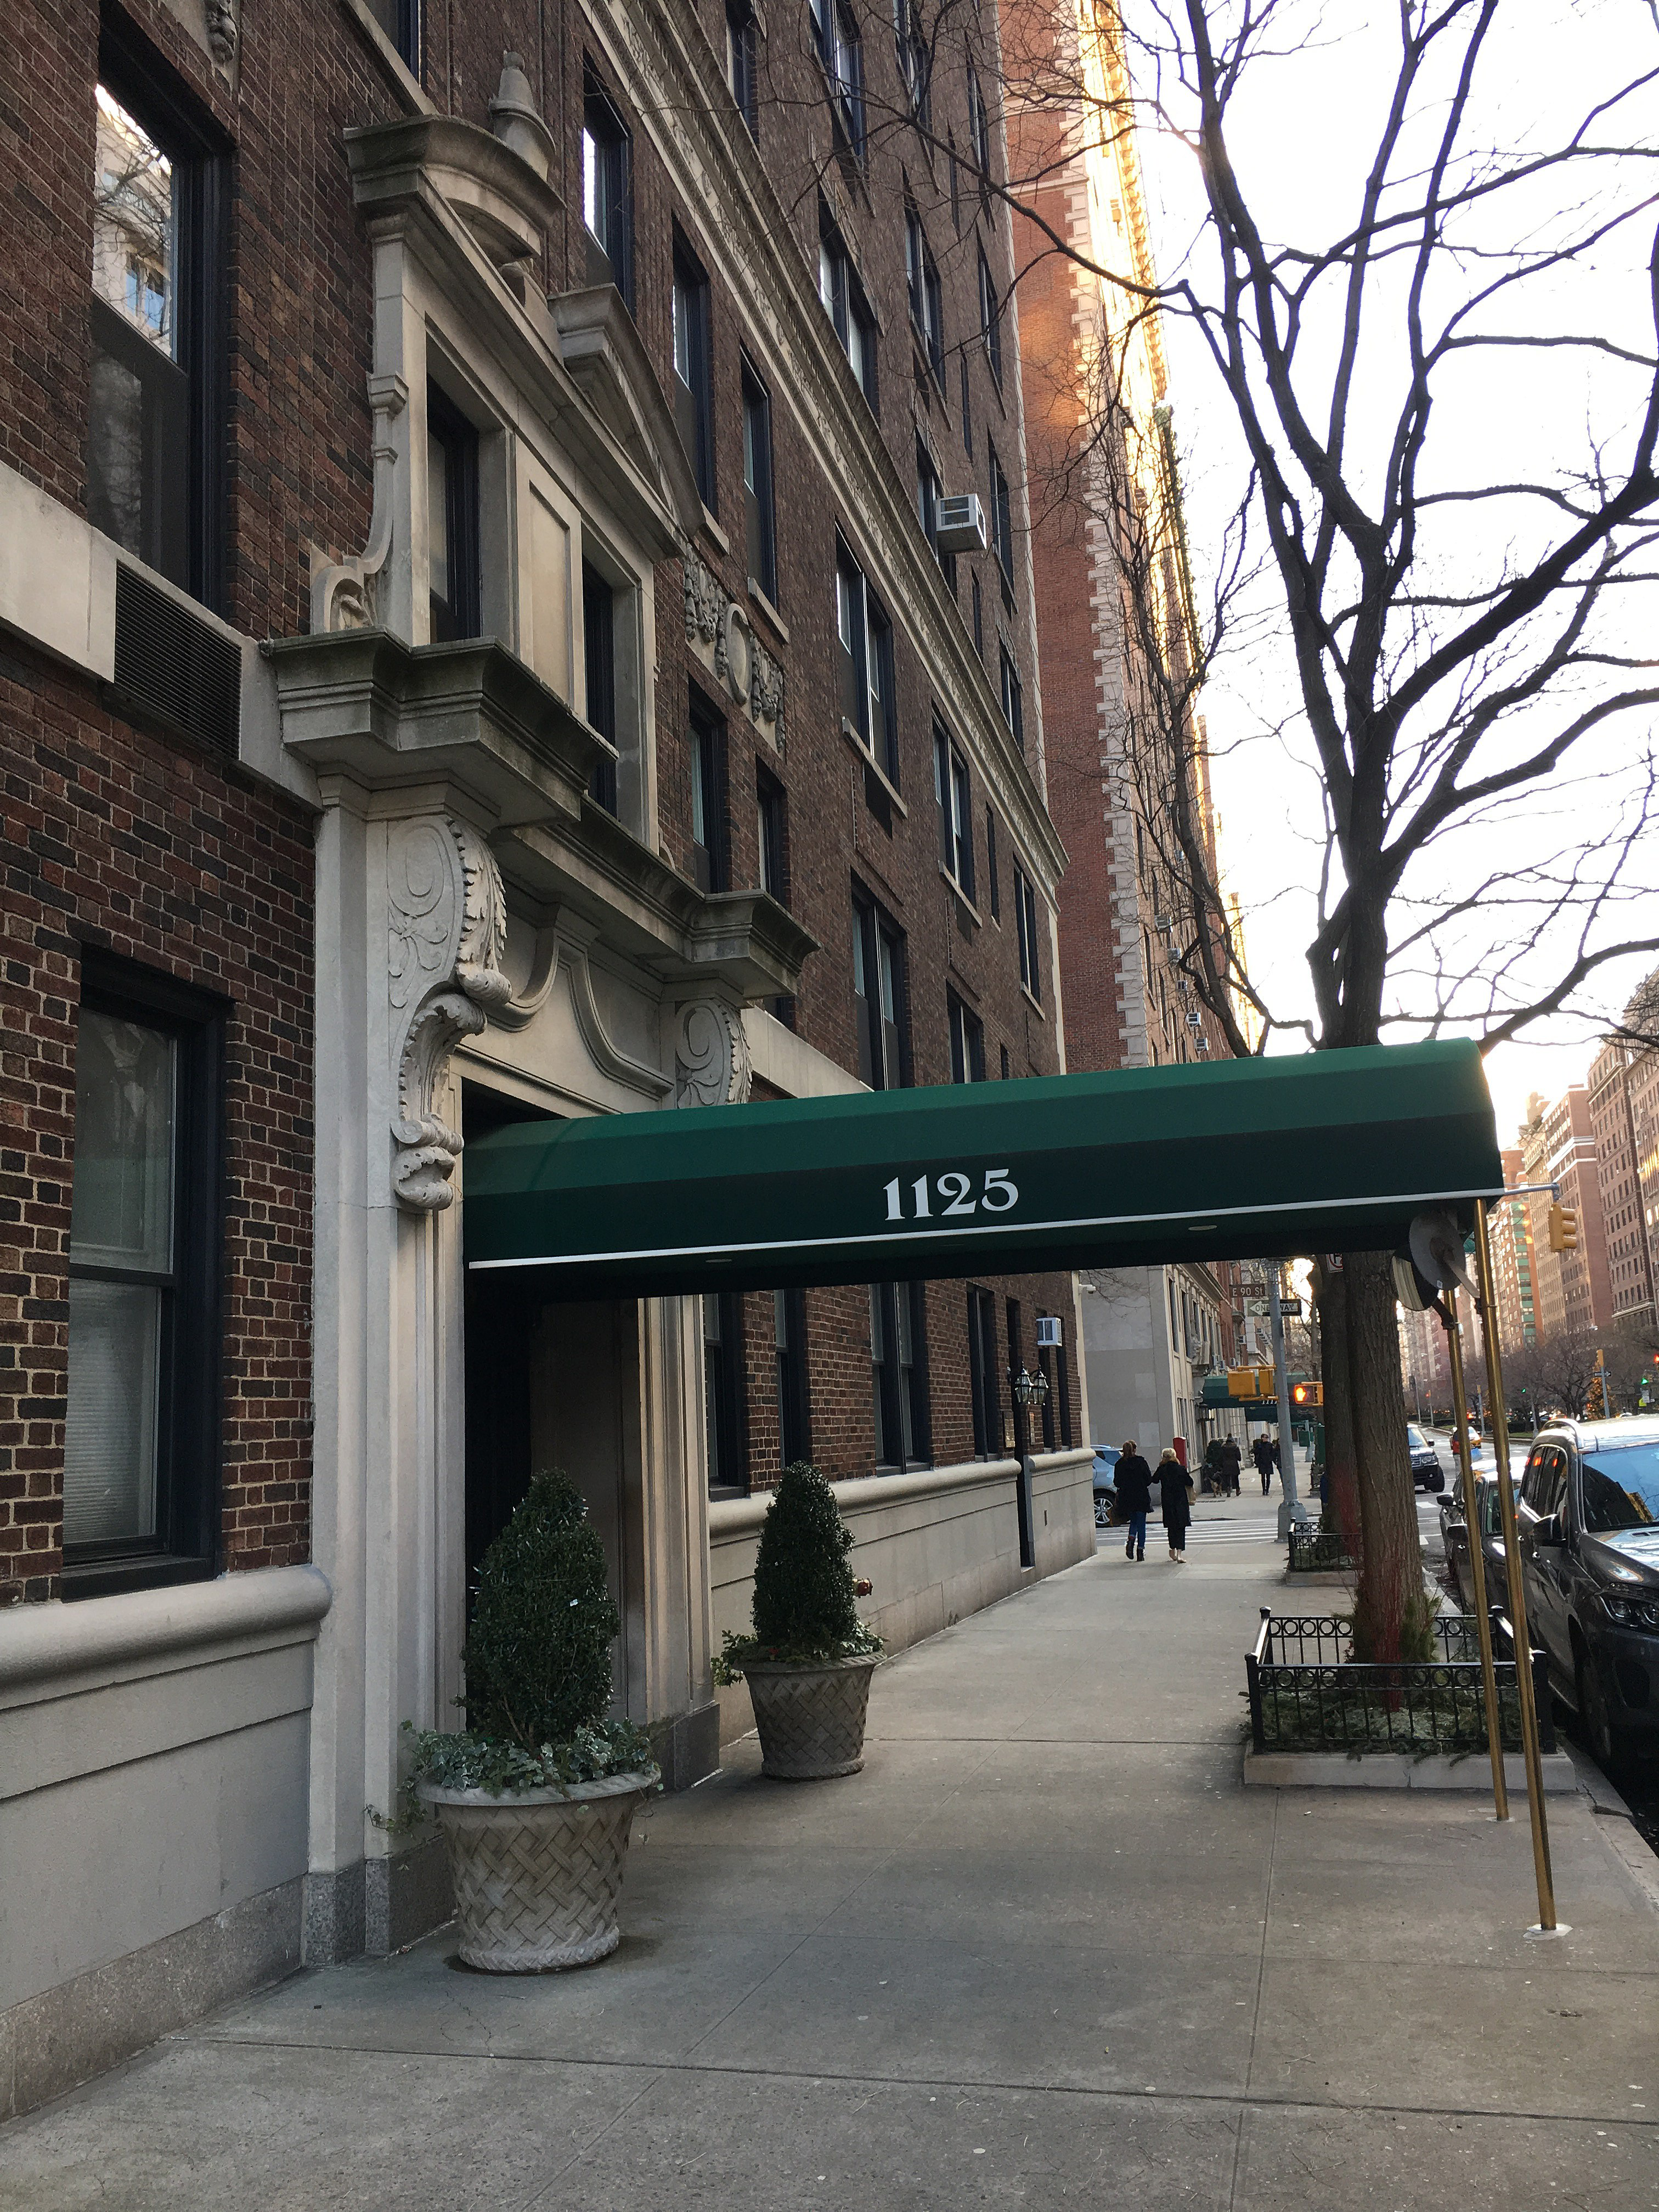
\includegraphics[width=4.5cm, height=4.cm]{chapter3/figure1-18}} node[rotate=90, font=\tiny] at ([yshift=.5cm,xshift=.1cm]b.south east) {\textsuperscript{\textcopyright} wikipedia} ;
\node[text width=5cm, fontscale=0.1] at ([yshift=0.5cm]b.north) {\mytriangle{red}{\small Traveling waves}};


 \node (c) at (12cm,0) {\includegraphics[width=4cm, height=4cm]{chapter3/figure1-19}} node[rotate=90, font=\tiny] at ([yshift=.5cm,xshift=.1cm]c.south east) {\textsuperscript{\textcopyright} PxHere} ;
\node[text width=5cm] at ([yshift=0.5cm]c.north) {\mytriangle{red}{\small Light is a wave}};

%
% \node (d) at (18cm,0) {\includegraphics[width=5cm, height=5cm]{chapter2/figure1-10}} node[rotate=90, font=\tiny] at ([yshift=.5cm,xshift=.1cm]c.south east) {\textsuperscript{\textcopyright} Needpix} ;
%\node[text width=4cm] at ([yshift=0.8cm]c.north) {\mytriangle{red}{\small Heat is thermal energy}};
\end{tikzpicture}
\end{minipage}

%%%%%%%%%%%%%%%%%%%%%%%%%%%%%%%%%%

%\newpage

\item[\docfilehook{Types and color of radiation}{}] 
Depending on its frequency--or on its wavelength--radiation can be classified as gamma rays, x rays, ultraviolet (UV), visible, infrared (IR), microwaves or radio waves. For example, radiation with wavelength of $10^{-2}$ nm belongs to gamma rays radiation, whereas radiation with wavelength of $10^{4}$ nm belongs to the Infrared. Gamma rays are the most energetic type of radiation, whereas radio waves are the less energetic waves. At the same time, radio waves have the largest wavelength.



\tikzstyle{every picture}+=[remember picture]
\tikzstyle{na} = [baseline=-.5ex]
\stepcounter{figurenewcounter}   \refstepcounter{figure}  \label{Fig:{\chapterlabel}\thefigurenewcounter} \begin{center}
\begin{tikzpicture}[fill between/on layer={axis grid}, line width=1pt, xscale=1,yscale=1, every node/.style={scale=0.9}]


\begin{axis}[
legend columns=-1,
 xlabel={\small $\lambda$, nm},
xticklabel style = {font=\tiny,yshift=0.2ex},
minor tick style={draw=none},
xmin=10^-4,
xmax=10^12	,
xtick distance=10^2,
xticklabel pos=top,
%x unit=\si{\nano\meter},
xmode=log,
ymin=0,
ymax=1,
major tick length=1.5cm,
height=3cm,
yticklabels={},
ytick=\empty,
legend cell align=left,
legend style={at={(0.85,3.77)},anchor=north}
]
\addplot[draw=none, name path=start, forget plot] coordinates{(10^-4,0)(10^-4,1)} ;
\addplot[draw=none, name path=gamma, forget plot] coordinates{(10^-3,0)(10^-3,1)} node[font=\tiny,white, above, sloped, pos = .5] {Gamma Rays};
\addplot[draw=none, name path=xrays, forget plot] coordinates{(10^-1,0)(10^-1,1)} node[font=\tiny,white, above, sloped, pos = .5] {X-Rays};
\addplot[draw=none, name path=uv, forget plot] coordinates{(400,0)(400,1)} ;
\addplot[draw=none, name path=visible, forget plot] coordinates{(700,0)(700,1)};
\addplot[draw=none, name path=ir, forget plot] coordinates{(10^1,0)(10^1,1)} node[font=\tiny,white, above, sloped, pos = .5] {UV};
\addplot[draw=none,  forget plot] coordinates{(10^4,0)(10^4,1)} node[font=\tiny,white, above, sloped, pos = .5] {IR} ;
%node[font=\tiny,black, above, sloped, pos = .5, yshift=6cm, xshift=3em, rotate=-90] {\small $\lambda$, nm};
\addplot[draw=none,  forget plot] coordinates{(10^7,0)(10^7,1)} node[font=\tiny,white, above, sloped, pos = .5] {Microwaves};
\addplot[draw=none,  forget plot] coordinates{(10^11,0)(10^11,1)} node[font=\tiny,white, above, sloped, pos = .5] {Radiowaves}  ;
\addplot[draw=none, name path=radiowave, forget plot] coordinates{(10^12,0)(10^12,1)};
\addplot[back, area legend] fill between[of=start and radiowave];
%\addlegendentry{$\nu$-ray}
%\addplot[black, area legend] fill between[of=gamma and xrays];
%%\addlegendentry{X-ray}
%\addplot[black, area legend] fill between[of=xrays and uv];
%%\addlegendentry{Ultra violet}
%\addplot[shading=visiblelight, area legend] fill between[of=uv and visible];
%%\addlegendentry{Visible light}
%\addplot[black, area legend] fill between[of=visible and ir];
%%\addlegendentry{Infrared}
%\addplot[black, area legend] fill between[of=ir and microwave];
%%\addlegendentry{Micro wave}
%\addplot[black, area legend] fill between[of=visible and radiowave];
%\addlegendentry{Radio wave}
\end{axis}


\pgfmathsetmacro{\oxa}{27}
\pgfmathsetmacro{\oxb}{1}
\pgfmathsetmacro{\oxc}{10}

\begin{scope}[xshift =10em, yshift =0em, scale=1]

\foreach \x in {0,...,12}
{
 \pgfmathsetmacro{\oxaa}{-8+ \oxa / 13 *\x}
   \pgfmathsetmacro{\oxaaa}{\oxaa +  \oxa / 13 *1}
  \pgfmathsetmacro{\oxbb}{2+ \oxb / 13 *\x}
  \pgfmathsetmacro{\oxbbb}{\oxbb +  \oxb / 13 *1}
\draw [draw=none, thin, black, dotted, shading=shading\x ,  shading angle=225, fill opacity=0.8] 	(\oxbb em,4em) --   (\oxbb em,0em) --  	      (\oxaa em,-5em)  -- (\oxaa em,-10 em)  --    (\oxaaa em,-10em) -- (\oxaaa em,-5 em) --   (\oxbbb em,0em)  --          (\oxbbb em,4em) -- cycle ;
}
\draw[thin] (-8 em,-5em) rectangle  (19 em,-10em);
\draw[thin]  (-8 em,-10em) --++ (0 em,-0.5em) node[yshift=-0.5em] {\small 400};
\draw[thin]  (1 em,-10em) --++ (0 em,-0.5em) node[yshift=-0.5em] {\small 500} node [yshift=-0.5em,xshift=4em]  {$\lambda$, nm} node [rotate=90, yshift=-1.5em,xshift=12.5em]  {\tiny\color{white}Visible spectrum};
\draw[thin]  (10 em,-10em) --++ (0 em,-0.5em) node[yshift=-0.5em] {\small 600};
\draw[thin]  (19 em,-10em)  --++ (0 em,-0.5em) node[yshift=-0.5em] {\small 700};

 \end{scope}

\begin{scope}[xshift =30em, yshift =-5em, scale=1]
\begin{axis}[hide axis,red,width=12cm,height=3.5cm,thick] 
\pgftransformrotate{180}
\addplot[white, domain=20:200,samples=800,thick, point meta=x*x]{sin(pow(x,2)/10)};
\end{axis}
 \end{scope}
 
\begin{scope} 
%%%%%%%%%%%%%%%%%%%%%%%%%%%%
\coordinate (spy point) at (19em,3em);
\coordinate (magnifying glass) at (19em,7em);
\node [draw=none, shape=circle, inner sep=1.5em, postaction={decorate,decoration={raise=-0.6em, text along path,text align=right,text={|\tiny\color{black}|{\textsuperscript{\textcopyright}} Flickr}}}]  (a) at (magnifying glass) {};
\draw[draw=none, fill=gray, fill opacity=0.2] (spy point) to [bend right=45] (a.west) -- (a.east)  to [bend left=45]  (spy point) -- cycle;
\node  [thin, draw=black, shape=circle, inner sep=1.5em, fill overzoom image=chapter3/figure1-10]  (c) at (magnifying glass) {} node[yshift=0.5em] at (c.north) {\tiny Heat lamp};
%%%%%%%%%%%%%%%%%%%%%%%%%%%%
\coordinate (spy point) at (23em,2em);
\coordinate (magnifying glass) at (25em,8em);
\node [draw=none, shape=circle, inner sep=1.5em, postaction={decorate,decoration={raise=-0.6em, text along path,text align=right,text={|\tiny\color{black}|{\textsuperscript{\textcopyright}} Flickr}}}]  (a) at (magnifying glass) {};
\draw[draw=none, fill=gray, fill opacity=0.2] (spy point) to [bend right=45] (a.west) -- (a.east)  to [bend left=45]  (spy point) -- cycle;
\node  [thin, draw=black, shape=circle, inner sep=1.5em, fill overzoom image=chapter3/figure1-14]  (c) at (magnifying glass) {} node[yshift=0.5em] at (c.north) {\tiny cell phone};
%%%%%%%%%%%%%%%%%%%%%%%%%%%%
%%%%%%%%%%%%%%%%%%%%%%%%%%%%
\coordinate (spy point) at (0em,3em);
\coordinate (magnifying glass) at (0em,8em);
\node [draw=none, shape=circle, inner sep=1.5em, postaction={decorate,decoration={raise=-0.6em, text along path,text align=right,text={|\tiny\color{black}|{\textsuperscript{\textcopyright}} Wikipedia}}}]  (a) at (magnifying glass) {};
\draw[draw=none, fill=gray, fill opacity=0.2] (spy point) to [bend left=45] (a.west) -- (a.east)  to [bend right=45]  (spy point) -- cycle;
\node  [thin, draw=black, shape=circle, inner sep=1.5em, fill overzoom image=chapter3/figure1-13]  (c) at (magnifying glass) {} node[yshift=0.5em] at (c.north) {\tiny nuclear plant};
%%%%%%%%%%%%%%%%%%%%%%%%%%%%
%%%%%%%%%%%%%%%%%%%%%%%%%%%%
\coordinate (spy point) at (6em,3em);
\coordinate (magnifying glass) at (6em,7.5em);
\node [draw=none, shape=circle, inner sep=1.5em, postaction={decorate,decoration={raise=-0.6em, text along path,text align=right,text={|\tiny\color{black}|{\textsuperscript{\textcopyright}} Wikipedia}}}]  (a) at (magnifying glass) {};
\draw[draw=none, fill=gray, fill opacity=0.2] (spy point) to [bend left=45] (a.west) -- (a.east)  to [bend right=45]  (spy point) -- cycle;
\node  [thin, draw=black, shape=circle, inner sep=1.5em, fill overzoom image=chapter3/figure1-12]  (c) at (magnifying glass) {} node[yshift=0.5em] at (c.north) {\tiny X rays};
%%%%%%%%%%%%%%%%%%%%%%%%%%%%

%%%%%%%%%%%%%%%%%%%%%%%%%%%%
\coordinate (spy point) at (20em,1em);
\coordinate (magnifying glass) at (29em,-2em);
\node [draw=none, shape=circle, inner sep=1.5em, postaction={decorate,decoration={raise=-0.6em, text along path,text align=right,text={|\tiny\color{black}|{\textsuperscript{\textcopyright}} cartalk.com}}}]  (a) at (magnifying glass) {};
\draw[draw=none, fill=gray, fill opacity=0.2] (spy point) to [bend right=45] (a.south) -- (a.north)  to [bend left=45]  (spy point) -- cycle;
\node  [thin, draw=black, shape=circle, inner sep=1.5em, fill overzoom image=chapter3/figure1-16]  (c) at (magnifying glass) {} node[yshift=-0.5em] at (c.south) {\tiny radars};
%%%%%%%%%%%%%%%%%%%%%%%%%%%%

%%%%%%%%%%%%%%%%%%%%%%%%%%%%
\coordinate (spy point) at (10em,1em);
\coordinate (magnifying glass) at (1em,-2em);
\node [draw=none, shape=circle, inner sep=1.5em, postaction={decorate,decoration={raise=-0.6em, text along path,text align=right,text={|\tiny\color{black}|{\textsuperscript{\textcopyright}} Flikr}}}]  (a) at (magnifying glass) {};
\draw[draw=none, fill=gray, fill opacity=0.2] (spy point) to [bend left=45] (a.north) -- (a.south)  to [bend right=45]  (spy point) -- cycle;
\node  [thin, draw=black, shape=circle, inner sep=1.5em, fill overzoom image=chapter3/figure1-15]  (c) at (magnifying glass) {} node[yshift=-0.5em] at (c.south) {\tiny tanning lights};
%%%%%%%%%%%%%%%%%%%%%%%%%%%%

\node[xshift=25em, yshift=-10em, text width=14cm, fontscale=0.1] at (-8em,-5em) { \begin{bf}\color{black}\bfseries\large Figure \ref{Fig:{\chapterlabel}\thefigurenewcounter} \end{bf} Spectrum of the electromagnetic radiation, from gamma rays (shortest wavelength) to radio waves (highest wavelength). The visible part of the spectrum ranges from 400 nm (violet) to 700 nm(red).   };
      \end{scope}
   
\end{tikzpicture}\end{center}






Light not always have color. Only a small range of wavelengths belong to visible radiation and the visible spectrum correspond to the set of visible frequencies. This means you will not be able to see for example, IR radiation or gamma rays. The color of the radiation is also dependent on the wavelength--of the frequency as both are related--and for example $\lambda=450$ nm will be blue light. Ultraviolet radiation is the most energetic visible radiation whereas infra red waves are the less energetic waves of the visible spectrum.
%\begin{marginfigure}[-0cm]%%%%%%%MARGIN FIGURE
%\begin{tcolorbox}[tab2,tabularx={>{\hsize=.4\hsize}X|X}]%%%% FANCY COLOR TABLE
% Radiation     &  $\nu$ (Hz)          \\\hline\hline
%Gamma  &   \small >$3\times 10^{19}$        \\\hline
%X-rays  &   \small $3\times 10^{19}-3\times 10^{16}$        \\\hline
%UV  &   \small $3\times 10^{16}-8\times 10^{14}$        \\\hline
%IR  &   \small $4\times 10^{14}-4\times 10^{11}$        \\\hline
%MicroW &   \small $3\times 10^{11}-3\times 10^{8}$        \\\hline
%RadioW  &   \small $3\times 10^{8}-3\times 10^{3}$                     
%\end{tcolorbox}%%%% FANCY COLOR TABLE
% \end{marginfigure}%%%%%%%MARGIN FIGURE
%
%
%
%
%\begin{marginfigure}[2cm]%%%%%%%MARGIN FIGURE
%\begin{tcolorbox}[tab2,tabularx={X|X}]%%%% FANCY COLOR TABLE
% Color     &  $\lambda$ (nm)          \\\hline\hline
%Violet  &   \small 380-450       \\\hline
%Blue  &   \small 450-485         \\\hline
%Cyan  &   \small 485-500        \\\hline
%Green &    \small 500-565      \\\hline
%Yellow &    \small 565-590        \\\hline
%Orange  &   \small 590-625   \\\hline     
%Red  &   \small 625-740                               
%\end{tcolorbox}%%%% FANCY COLOR TABLE
%
% \end{marginfigure}%%%%%%%MARGIN FIGURE


\begin{center}
\refstepcounter{table}  \label{tab:{\chapterlabel}4}
\fontfamily{ppl}\selectfont
\begin{tabular}{lllcll}
\rowcolor{black!45}
\toprule
\multicolumn{5}{l}{\hypersetup{colorlinks,linkcolor={white}} \cellcolor{black}\color{white}\bfseries\small Table \ref{tab:electrolytes4} Types and color of radiation } \\
\midrule
\rowcolor{gray!45} Type of radiation  &  $\nu$ (Hz)  &\multicolumn{1}{l}{} &Color of radiation & $\lambda$ (nm)     \\
 \midrule
Gamma  &   \small >$3\times 10^{19}$     				&\multicolumn{1}{l}{} &Violet &   \small 380-450						  \\
X-rays  &   \small $3\times 10^{19}-3\times 10^{16}$      & \multicolumn{1}{l}{} &	Blue	&   \small 450-485 		   \\
UV  &   \small $3\times 10^{16}-8\times 10^{14}$        	&\multicolumn{1}{l}{}  &Cyan		&   \small 485-500 	 \\
IR  &   \small $4\times 10^{14}-4\times 10^{11}$        		&\multicolumn{1}{l}{}  &Green	&    \small 500-565		 \\
MicroW &   \small $3\times 10^{11}-3\times 10^{8}$       	&\multicolumn{1}{l}{}  &Yellow	&    \small 565-590  		   \\
RadioW  &   \small $3\times 10^{8}-3\times 10^{3}$    	&\multicolumn{1}{l}{}  &	Orange	&   \small 590-625	  \\               
      						&				  	&\multicolumn{1}{l}{}  &	Red	&   \small 625-740	  \\  
 \bottomrule

\end{tabular}\end{center} 


\begin{example} %%%%%%%%%%%%%%%%%%%%%%%% EXAMPLE BOX
Indicate: (a) the color of a radiation with $\lambda=650nm$; (b) the type of a radiation with  $\lambda=10^{5}$ nm; (c) the type of a radiation with  $\nu=10^{16}$ Hz.\\
\textlcsc{ \textcolor{dgreen}{\Large \textbf{Solution}} }\\
We can answer the first questions by inspecting the figure above we can see that $\lambda=650nm$ corresponds to red radiation. To answer the second question we will also use the figure above, where we can see that $\lambda=10^{5}$ nm belongs to the infrared. Finally, in order to answer the last question we need to convert frequency into wavelength, as the figure above only indicates wavelength. $\nu=10^{16}$ Hz corresponds to $\lambda=30$ nm. Hence, this frequency corresponds to the UV.
\\
\faDiamond\ \textlcsc{ \textcolor{dgreen}{\Large \textbf{Study Check}} }\\
Indicate: (a) the color of a radiation with $\nu=7.5\times 10^{14}$ Hz; (b) the type of a radiation with  $\nu=10^{8}$ Hz.
\flushright Answer: (a) violet; (b) Microwaves.
\end{example}%%%%%%%%%%%%%%%%%%%%%%%% EXAMPLE BOX








\item[\docfilehook{Electron-Volt a new unit of energy}{Electron-Volt a new unit of energy}]
 Sometimes, it is convenient to use another energy unit, called electron-volt, that makes these values have more reasonable values.%\resizeableyellownote{2.5}{1}{Add this formula to your flashcard.}
\begin{equation*}
\boxed{    1 eV=1.60218\times 10^{-19} J   } \qquad\text{or}\qquad  \boxed{\frac{1 eV}{1.60218\times 10^{-19} J }}  
\end{equation*}
For example, the energy in eV of the first level is $E_1=-13.6eV$, whereas the energy of the third level is $E_3=-1.5J$.

\item[\docfilehook{The photoelectric effect}{ }]
The photoelectric effect was a mysterious phenomena discovered early in the twentieth century. Scientist found that if you expose a metal to light, under certain conditions, it emits electrons--it produced electricity. They found that the intensity--the brightness--of the radiation was not a key component of this phenomena, and not by increasing the intensity you were able to produce electrons. 
\stepcounter{figurenewcounter}   \refstepcounter{figure}  \label{Fig:{\chapterlabel}\thefigurenewcounter}
\begin{center}
\begin{tikzpicture}
\begin{scope}[shift={(-3,0)}]
  \draw[gray,fill=gray,path fading=south] (0,0) rectangle +(5,-2);% sample
    \begin{scope}[decoration={snake,amplitude=.4mm,
        segment length=2mm,post length=1mm}]
%       \draw[decorate,blue,->] (2.5,0) -- ++(112:3);% x-ray
%      \draw[decorate,red,->] (2.5,0) -- ++(5:2);% auger
      \draw[decorate,orange,->] (2.5,0) -- ++(45:3) node (ele) {} ;% cathodlimuescence
\fill[ball color=gray!30] (ele) circle (3pt) node  {\texttt{-}};
    \end{scope}
%  \fill[color=red, path fading=north,fading transform={rotate=-15}]
%    (2.5,0) ++(60:3) ++(150:0.1) -- ++(-30:0.2) -- (2.5,0) -- cycle;%backscatter
%  \fill[color=green, path fading=north,fading transform={rotate=45}]
%    (2.5,0) ++(135:2) ++(225:0.3) -- ++(45:0.6) -- (2.5,0) -- cycle;%secondary
  \shade[inner color=blue, top color=blue] (2.2,1.8)
    -- ++(0.6,0) -- ++(-0.3,-1.8) -- cycle;%primary electrons

  \shade[left color=gray!50!white,right color=gray] (1.7,3)
    -- ++(1.6,0) -- ++(-0.3,-1) -- ++(-1,0) -- cycle;% column
  \shade[left color=gray!50!white,right color=gray] (2.1,2)
    -- ++(0.8,0) -- ++(0,-0.2) -- ++(-0.8,0) -- cycle;% column bottom
  \draw[gray!80!black] (1.7,3) -- ++(1.6,0) -- ++(-0.3,-1)
    -- ++(-1,0) -- cycle;%column
  %    \path (0,-2) pic {disc bottom} ;
%
  \draw[gray!80!black] (2.1,2) -- ++(0,-0.2) -- ++(0.8,0)
     -- ++(0,0.2);%column bottom
%		
%  \shade[left color=gray!50!white,right color=gray] (2.5,0) ++(135:2) --
%    ++(225:0.3) -- ++(135:0.8) -- ++(45:0.6) -- ++(315:0.8) -- cycle;% detector
		
  %labels
  \draw (0,-2) node[above right] {\footnotesize Metal {\small (Workfunction=W)}};
%  \draw (2.5,0) ++(5:2) node[right] {\footnotesize Auger};
  \draw (2.5,0) ++(45:3) node[right] {\footnotesize Electron};
    \draw (2.5,0) ++(45:1) node[right] {\footnotesize KE};
  \draw (1.75,1.4) node[above right] {\footnotesize  $h\nu$};

%  \draw (2.5,0) ++(60:3) node[right] {\footnotesize Backscattered};
%  \draw (2.5,0) ++(112:3) node[left] {\footnotesize X-ray};
%  \draw (2.5,0) ++(135:1.2) node[left=0.4cm] {\footnotesize Secondary};
%  \draw (2.5,0) ++(135:2) ++(225:0.3) ++(135:0.8) node[left]
    {\footnotesize Detector};
    \end{scope}
    \node[text width=12cm, fontscale=0.1] at (0em,-8em) { \begin{bf}\color{black}\bfseries\large Figure \ref{Fig:{\chapterlabel}\thefigurenewcounter} \end{bf} The photoelectric effect: when light with frequency ($\nu$) larger than a threshold irradiates a metal, electrons are ejected with a specific kinetic energy (KE) that depends on the work function (W) of the metal.   };

\end{tikzpicture}\end{center}

They key was the frequency of the radiation. For frequencies above a specific threshold radiation was produce. If the frequency was above that threshold--called threshold radiation, $\nu_c$--then the larger the intensity of the radiation the more electrons were produced. On that time, the current theory of light, associating intensity of light with energy, was unable to explain this phenomena. Albert Einstein used Plank's theory of the blackbody radiation to solve this mystery.
He assumed that light is made of a steam of particles called photons, each with a given energy, $h\nu$. The electrons of a metal are held by attractive forces. A property called work function $W$--or biding energy--tells how strongly the electrons of a metal are held together. 

\begin{center}
\refstepcounter{table}  \label{tab:{\chapterlabel}2}
\fontfamily{ppl}\selectfont
\begin{tabular}{lll}
\rowcolor{black!45}
\toprule
\multicolumn{3}{l}{\hypersetup{colorlinks,linkcolor={white}} \cellcolor{black}\color{white}\bfseries\small Table \ref{tab:{\chapterlabel}2} List of metal workfunctions and threshold frequencies } \\
\midrule
 \rowcolor{gray!10} \multicolumn{1}{c}{Element} & \multicolumn{1}{c}{W (eV)} &\multicolumn{1}{c}{$\nu_c$, Hz}     \\
\midrule
    \multicolumn{1}{c}{Ag}	&	 \multicolumn{1}{c}{4.64} 	&			\multicolumn{1}{c}{$1.1\times 10^{15}$}	  \\
     \multicolumn{1}{c}{Ba}	& \multicolumn{1}{c}{2.52 }	&		\multicolumn{1}{c}{$6.1\times 10^{14}$}			  \\
        \multicolumn{1}{c}{Fe}	& \multicolumn{1}{c}{4.67} 	&		\multicolumn{1}{c}{$1.1\times 10^{15}$}			  \\
\multicolumn{1}{c}{Al	}&	 \multicolumn{1}{c}{4.20	}		&\multicolumn{1}{c}{$1.0\times 10^{15}$}\\
\multicolumn{1}{c}{Ca}	& \multicolumn{1}{c}{2.87}	&\multicolumn{1}{c}{$6.9\times 10^{14}$}\\
\multicolumn{1}{c}{Mn}			& \multicolumn{1}{c}{4.1	}	&\multicolumn{1}{c}{$9.9\times 10^{14}$}\\
 \bottomrule

\end{tabular}\end{center} 




In Table \ref{tab:{\chapterlabel}2} you can find numerous workfunctions. Metals such as Fe have high workfunctions in comparison to metals such as Ca, that means it takes more energy to remove an electron from the metal.
Therefore, if the energy of the radiation was enough to overcome this forces, the electron emission will happen. In other words, if $h\nu$ is larger than $W$ the electron emission will happen and the electrons emitted will have a kinetic energy (KE) equal to:

\begin{equation*}
\boxed{  KE=4.13\times 10^{-15}\nu -W  } \quad \textcolor{blue}{\text{Photoelectric effect}}
\end{equation*}
where:
\begin{where}
 \item $KE$   is the kinetic energy of the emitted electrons in eV
  \item $4.13\times 10^{-15}$ is called Plank's constant in eV$\cdot\text{ }$s, $h$
 \item $\nu$  is frequency in hertz (Hz)
 \item is the workfunction of the metal in eV
\end{where}
What is the threshold frequency, $\nu_c$? When the energy of the radiation is the same as the work-function of the metal, then electrons are ejected. This way, the threshold frequency is just the work-function of the metal converted in units of frequency:
\begin{equation*}
\boxed{ \nu_c =\frac{W}{4.13\times 10^{-15}}  } \quad \textcolor{blue}{\text{threshold frequency}}
\end{equation*}
$4.13\times 10^{-15}$ is called Plank's constant in eV$\cdot\text{ }$s, $h$, $\nu_c$  is the threshold frequency in hertz (Hz) and $W$ is the workfunction of the metal in eV.
Einsteins theory of the photoelectric effect shocked the scientific community. Before this theory, light was considered a wave. Based on Einstein's theory, wave poses properties of both a particle and a wave, and depending on the experiment one experience light as a wave or as a particle.






\begin{example} %%%%%%%%%%%%%%%%%%%%%%%% EXAMPLE BOX
A metal with workfunction of 5eV is exposed to a radiation source with frequency of $2\times 10^{15}$Hz. Indicate whether electrons will be ejected and if so, indicate the kinetic energy of these. \\
\textlcsc{ \textcolor{dgreen}{\Large \textbf{Solution}} }\\
Using the photoelectric effect equation we have that a radiation of $10^{15}$Hz frequency has an energy of 
\[4.13\times 10^{-15} \cdot 2\times 10^15=8.27eV\]
As this values is larger than the workfunction of the metal (W=5eV), therefore electrons will be ejected with a kinetic energy of:
\[KE=8.27-5=3.27eV\]
\faDiamond\ \textlcsc{ \textcolor{dgreen}{\Large \textbf{Study Check}} }\\
A metal with workfunction of 5eV is exposed to a radiation source with frequency of $9\times 10^{14}$Hz. Indicate whether electrons will be ejected and if so, indicate the kinetic energy of these. \\
\flushright Answer: no electrons will be ejected
\end{example}%%%%%%%%%%%%%%%%%%%%%%%% EXAMPLE BOX








\end{description}
 
\section{The atomic line spectra}
This section will explain the atomic spectra of atoms and in particular, hydrogen. Atoms emit light, but not any type of light as they emit specific frequencies of radiation. The atomic spectrum is a representation of the different wavelengths of the radiation emitted--or absorbed--by an atom. This section will gain insight into the reasons for the emission of specific frequencies of light and will introduce the Bohr model that justifies the lines in the atomic spectrum of hydrogen.
\sloppy
\begin{description}
\item[\docfilehook{Spectrum of atoms}{ }]
The absorption spectrum of an atom is a representation of the different frequencies in which an atom absorbs or emits radiation. Each atoms has a distinctive emission spectrum. Some of these lines correspond to the visible spectrum, that is, they can be seen. Others correspond higher or lower parts of the spectrum. This section will cover the spectrum of hydrogen. 
\stepcounter{figurenewcounter}   \refstepcounter{figure}  \label{Fig:{\chapterlabel}\thefigurenewcounter}
     \begin{center}\begin{tikzpicture}[xscale=1,yscale=0.8, every node/.style={scale=1}]
            \node (a) at (0,0) {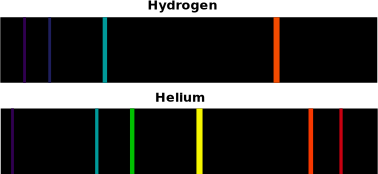
\includegraphics[width=8cm]{chapter3/figure1-21}} node[rotate=90, font=\tiny] at ([yshift=.5cm,xshift=.1cm]a.south east) {\textsuperscript{\textcopyright} wikipedia} ;
 \node[text width=12cm, fontscale=0.1, shift={ (5em,-7em)}] at (0em,0em) { \begin{bf}\color{black}\bfseries\large Figure \ref{Fig:{\chapterlabel}\thefigurenewcounter} \end{bf} Atomic spectrum of two atoms showing the lines corresponding to the visible.   };
\end{tikzpicture}\end{center}





\item[\docfilehook{Atomic line spectrum of hydrogen}{}]
Newton shown that sunlight (white light) is composed of various components of different colors. Similar type of radiation called emission spectra can be produced by heating a substance. Think for example of a hot piece of metal. Both the sun and a heated piece of metal have in common the fact that their spectrum is continuous and contains all wavelengths of visible light.
We can achieve a similar effect by applying a high-voltage electrical discharge to a gas.
  \\
%\vspace{4cm}
%\begin{tikzpicture} [transform canvas={scale=0.6}]
\begin{center}\begin{tikzpicture}[thin,scale=0.6, every node/.style={scale=0.6}]
\begin{scope}[shift={(0,.8)}]
  \fill[blue!60!green!70] (0,0) -- (4,0) -- (1.7,-1.8) -- cycle;
  \fill[blue!60!green!70,opacity = 0.2]  (1.7,-1.8) --(1.7,-4) -- (0,-2) -- (0,0);
    \fill[blue!60!green!70,opacity = 0.6]  (1.7,-4) -- (4,-2) -- (4,-1.8) --(4,0) --(1.7,-1.8) ;
    \node[shift={(3.5,0.5)}] {Prism};
\end{scope}
\begin{scope}[x={(1,0)},y={(0,1)},z={({cos(60)},{sin(60)})},
font=\sffamily\small,scale=0.9, shift={(-3.1,-4.1)}]
 \draw[gray,ultra thin,fill=green]  (0,0,0) coordinate(-front-bottom-left) to
++ (0,4,0) coordinate(-front-top-right) --++
(0.1,0,0) coordinate(-front-top-right) --++ (0,-4,0) 
coordinate(-front-bottom-right) -- cycle;
\draw[gray,ultra thin,fill=green] (0,4,0)  --++ 
 (0,0,1) coordinate(-back-top-left) --++ (0.1,0,0) 
 coordinate(-back-top-right) --++ (0,0,-1)  -- cycle;
\draw[gray,ultra thin,fill=green!40!black] (0.1,0,0) --++ (0,0,1) coordinate(-back-bottom-right)
--++ (0,4,0) --++ (0,0,-1) -- cycle;
\draw[gray,ultra thin,fill=green!10!black, shift={(-0.6,2)}] (1,0,0) --++ (0,0,.1) coordinate(-back-bottom-right)
--++ (0,1.1,0) --++ (0,0,-.1) -- cycle;
\node[shift={(0.5,-0.5)}] {slit};
\end{scope}
\begin{scope}[transform canvas={scale=1},overlay, shift={(-0,-0)}]
 \pgfmathsetmacro{\arainbow}{-3}
 \pgfmathsetmacro{\brainbow}{0.5}
\fill[fill=none, draw=black] (-2.4,-1.9) rectangle (0.8,-0.9);
\draw[shift={(3,-1.5)}, draw=none] (0,0) -- (3,2) --(3,3) -- (0,1) -- cycle;
\draw[shift={(3,-1.5)}] (3,2) -- (6,1.5) --(6,2.5) -- (3,3) -- cycle;
\draw[shift={(3,-1.5)}, fill=red!80, draw=none, opacity=0.5]  (6,1.5) --(0,.0) -- (0,1) --(6,2.5) -- cycle;
 \pgfmathsetmacro{\arainbowaa}{6+0*\arainbow /7}
  \pgfmathsetmacro{\brainbowbb}{2.5+0*\brainbow /7}
   \pgfmathsetmacro{\arainbowa}{1*\arainbow /7}
  \pgfmathsetmacro{\brainbowb}{1*\brainbow /7}
\draw[shift={(3,-1.5)}, fill=red!80, draw=none, opacity=0.5] (0,1)-- (\arainbowaa,\brainbowbb) --++(\arainbowa,\brainbowb)  -- cycle;
 \pgfmathsetmacro{\arainbowaa}{6+1*\arainbow /7}
  \pgfmathsetmacro{\brainbowbb}{2.5+1*\brainbow /7}
   \pgfmathsetmacro{\arainbowa}{1*\arainbow /7}
  \pgfmathsetmacro{\brainbowb}{1*\brainbow /7}
\draw[shift={(3,-1.5)}, fill=orange!80, draw=none, opacity=0.5] (0,1)-- (\arainbowaa,\brainbowbb) --++(\arainbowa,\brainbowb)  -- cycle;
\pgfmathsetmacro{\arainbowaa}{6+2*\arainbow /7}
  \pgfmathsetmacro{\brainbowbb}{2.5+2*\brainbow /7}
   \pgfmathsetmacro{\arainbowa}{1*\arainbow /7}
  \pgfmathsetmacro{\brainbowb}{1*\brainbow /7}
\draw[shift={(3,-1.5)}, fill=yellow!80, draw=none, opacity=0.5] (0,1)-- (\arainbowaa,\brainbowbb) --++(\arainbowa,\brainbowb)  -- cycle;
\pgfmathsetmacro{\arainbowaa}{6+3*\arainbow /7}
  \pgfmathsetmacro{\brainbowbb}{2.5+3*\brainbow /7}
   \pgfmathsetmacro{\arainbowa}{1*\arainbow /7}
  \pgfmathsetmacro{\brainbowb}{1*\brainbow /7}
\draw[shift={(3,-1.5)}, fill=green!80, draw=none, opacity=0.5] (0,1)-- (\arainbowaa,\brainbowbb) --++(\arainbowa,\brainbowb)  -- cycle;
\pgfmathsetmacro{\arainbowaa}{6+4*\arainbow /7}
  \pgfmathsetmacro{\brainbowbb}{2.5+4*\brainbow /7}
   \pgfmathsetmacro{\arainbowa}{1*\arainbow /7}
  \pgfmathsetmacro{\brainbowb}{1*\brainbow /7}
\draw[shift={(3,-1.5)}, fill=blue!80, draw=none, opacity=0.5] (0,1)-- (\arainbowaa,\brainbowbb) --++(\arainbowa,\brainbowb)  -- cycle;
\pgfmathsetmacro{\arainbowaa}{6+5*\arainbow /7}
  \pgfmathsetmacro{\brainbowbb}{2.5+5*\brainbow /7}
   \pgfmathsetmacro{\arainbowa}{1*\arainbow /7}
  \pgfmathsetmacro{\brainbowb}{1*\brainbow /7}
\draw[shift={(3,-1.5)}, fill=cyan!80, draw=none, opacity=0.5] (0,1)-- (\arainbowaa,\brainbowbb) --++(\arainbowa,\brainbowb)  -- cycle;
\pgfmathsetmacro{\arainbowaa}{6+6*\arainbow /7}
  \pgfmathsetmacro{\brainbowbb}{2.5+6*\brainbow /7}
   \pgfmathsetmacro{\arainbowa}{1*\arainbow /7}
  \pgfmathsetmacro{\brainbowb}{1*\brainbow /7}
\draw[shift={(3,-1.5)}, fill=violet!80, draw=none, opacity=0.5] (0,1)-- (\arainbowaa,\brainbowbb) --++(\arainbowa,\brainbowb)  -- cycle;
    \node[shift={(7.5,1.8)}]   {Continous spectrum};

\end{scope}
\begin{scope}[transform canvas={scale=0.1},overlay, shift={(-35,-15)}]
     \node[shift={(-3 ,-15)},font=\fontsize{52}{58}\sffamily\bfseries] at (-0,0) {White light source};
 \draw  (-3,10) --(0,10) --(0,-10)  -- (-3,-10)  ;
  \draw  (0,0) --++(40:9.2)   ;
  \draw  (0,0) --++(-40:9.2)   ;
\draw (-3,-10) node[shift={(-1,0)},font=\fontsize{52}{58}\sffamily\bfseries]{+};
\draw (-3,10)node[shift={(-1,0)},font=\fontsize{52}{58}\sffamily\bfseries]{-};
\draw[shift={(-1,0)},] (-3,-10)  circle (1cm);
\draw[shift={(-1,0)},] (-3,10)  circle (1cm);
% \tstar{0.1}{3}{20}{1}{thick,fill=yellow}
\pgfmathsetmacro{\starangle}{360/20}
\draw[thick,fill=yellow, color=yellow] (1:0.1)
\foreach \x in {1,...,20}
{ -- (1+\x*\starangle-\starangle/2:3) -- (1+\x*\starangle:0.1)
}
-- cycle;
\end{scope}
  \begin{scope}[shift={(0,-6.5)}]
  \fill[blue!60!green!70] (0,0) -- (4,0) -- (1.7,-1.8) -- cycle;
  \fill[blue!60!green!70,opacity = 0.2]  (1.7,-1.8) --(1.7,-4) -- (0,-2) -- (0,0);
    \fill[blue!60!green!70,opacity = 0.6]  (1.7,-4) -- (4,-2) -- (4,-1.8) --(4,0) --(1.7,-1.8) ;
        \node[shift={(3.5,0.5)}] {Prism};
\end{scope}
 \begin{scope}[x={(1,0)},y={(0,1)},z={({cos(60)},{sin(60)})},
font=\sffamily\small,scale=0.9, shift={(-3.1,-11.9)}]
 \draw[gray,ultra thin,fill=green]  (0,0,0) coordinate(-front-bottom-left) to
++ (0,4,0) coordinate(-front-top-right) --++
(0.1,0,0) coordinate(-front-top-right) --++ (0,-4,0) 
coordinate(-front-bottom-right) -- cycle;
\draw[gray,ultra thin,fill=green] (0,4,0)  --++ 
 (0,0,1) coordinate(-back-top-left) --++ (0.1,0,0) 
 coordinate(-back-top-right) --++ (0,0,-1)  -- cycle;
\draw[gray,ultra thin,fill=green!40!black] (0.1,0,0) --++ (0,0,1) coordinate(-back-bottom-right)
--++ (0,4,0) --++ (0,0,-1) -- cycle;
\draw[gray,ultra thin,fill=green!10!black, shift={(-0.6,2)}] (1,0,0) --++ (0,0,.1) coordinate(-back-bottom-right)
--++ (0,1.1,0) --++ (0,0,-.1) -- cycle;
\node[shift={(0.5,-0.5)}] {slit};
\end{scope}
 \begin{scope}[transform canvas={scale=1},overlay, shift={(-0,-7)}]
 \pgfmathsetmacro{\arainbow}{-3}
 \pgfmathsetmacro{\brainbow}{0.5}
\fill[fill=none, draw=black] (-2.4,-1.9) rectangle (0.8,-0.9);
\draw[shift={(3,-1.5)}] (0,0) -- (3,2) --(3,3) -- (0,1) -- cycle;
\draw[shift={(3,-1.5)}] (3,2) -- (6,1.5) --(6,2.5) -- (3,3) -- cycle;
\draw[shift={(3,-1.5)}, fill=none, draw=black ]  (6,1.5) --(0,.0) -- (0,1) --(6,2.5) -- cycle;
 \pgfmathsetmacro{\arainbowaa}{6+1*\arainbow /7}
  \pgfmathsetmacro{\brainbowbb}{2.5+1*\brainbow /7}
   \pgfmathsetmacro{\arainbowa}{.5*\arainbow /7}
  \pgfmathsetmacro{\brainbowb}{.5*\brainbow /7}
\draw[shift={(3,-1.5)}, fill=orange!80, draw=none, opacity=0.5] (0,1)-- (\arainbowaa,\brainbowbb) --++(\arainbowa,\brainbowb)  -- cycle;
\draw[shift={(3,-1.5)}, fill=orange!80, draw=none, opacity=0.5] (0,1)-- (\arainbowaa,\brainbowbb) --++(0,-1) -- (0,0) -- cycle;

\pgfmathsetmacro{\arainbowaa}{6+5*\arainbow /7}
  \pgfmathsetmacro{\brainbowbb}{2.5+5*\brainbow /7}
   \pgfmathsetmacro{\arainbowa}{.5*\arainbow /7}
  \pgfmathsetmacro{\brainbowb}{.5*\brainbow /7}
 \draw[shift={(3,-1.5)}, fill=cyan!80, draw=none, opacity=0.5] (0,1)-- (\arainbowaa,\brainbowbb) --++(\arainbowa,\brainbowb)  -- cycle;
\draw[shift={(3,-1.5)}, fill=cyan!80, draw=none, opacity=0.5] (0,1)-- (\arainbowaa,\brainbowbb) --++(0,-1) -- (0,0) -- cycle;
    \node[shift={(7.5,-1.5)}] {Discrete spectrum};

\end{scope}
\begin{scope}[transform canvas={scale=0.1},overlay, shift={(-35,-15)}]
 \draw  (-3,10) --(0,10) --(0,-10)  -- (-3,-10)  ;
  \draw  (0,0) --++(40:9.2)   ;
  \draw  (0,0) --++(-40:9.2)   ;
\draw (-3,-10) node[shift={(-1,0)},font=\fontsize{52}{58}\sffamily\bfseries]{+};
\draw (-3,10)node[shift={(-1,0)},font=\fontsize{52}{58}\sffamily\bfseries]{-};
\draw[shift={(-1,0)},] (-3,-10)  circle (1cm);
\draw[shift={(-1,0)},] (-3,10)  circle (1cm);
 %\tstar{0.1}{3}{20}{1}{thick,fill=yellow}
 \pgfmathsetmacro{\starangle}{360/20}
\draw[thick,fill=yellow, color=yellow] (1:0.1)
\foreach \x in {1,...,20}
{ -- (1+\x*\starangle-\starangle/2:3) -- (1+\x*\starangle:0.1)
}
-- cycle;
\end{scope}
 \begin{scope}[transform canvas={scale=0.1},overlay, shift={(-35,-85)}]
      \node[shift={(-3 ,-15)},font=\fontsize{52}{58}\sffamily\bfseries] at (-0,0) {H gas discharge tube};

 \draw  (-3,10) --(0,10) --(0,3) ;
 \draw[line width=1mm,draw=red,decoration = {zigzag,segment length = 3mm, amplitude = 1mm},decorate] (0,3)--(0,-4);
\draw (0,-4) --(0,-10)  -- (-3,-10)  ;
  \draw  (1.5,1.5) --++(40:9.2)   ;
  \draw  (1.5,-1.5) --++(-40:9.2)   ;
\draw (-3,-10) node[shift={(-1,0)},font=\fontsize{52}{58}\sffamily\bfseries]{+};
\draw (-3,10)node[shift={(-1,0)},font=\fontsize{52}{58}\sffamily\bfseries]{-};
\draw[shift={(-1,0)},] (-3,-10)  circle (1cm);
\draw[shift={(-1,0)},] (-3,10)  circle (1cm);
  \draw	 [rounded corners=35pt,shift={(- 1.5,-4)}, fill=blue!40, draw=none, opacity=.2]  (0,0) rectangle ++(3,7);
  \draw[draw=red,rounded corners=35pt,shift={(- 1.5,-4)}, fill=none, draw=black] (0,0) rectangle ++(3,7);
  \draw[rounded corners=35pt,shift={(- 2. ,-4.5)}, fill=blue!40, draw=none, opacity=.2] (0,0) rectangle ++(4,8);
    \draw[line width=1mm,draw=red,rounded corners=35pt,shift={(- 1.6,-4.1)}, fill=none, draw=white] (0,0) rectangle ++(3.2,7.2);
\end{scope}
%%%%%%%%%%%%%%%%%%%%%%%%%%%%
\coordinate (spy point) at (20em,-17em);
\coordinate (magnifying glass) at (29em,-5em);;
\node [draw=none, shape=rectangle, minimum width=6cm,minimum height=1.3cm, postaction={decorate,decoration={raise=-0.6em, text along path,text align=right,text={|\tiny\color{black}|{\textsuperscript{\textcopyright}} Wikipedia}}}]  (a) at (magnifying glass) {};
\draw[draw=none, fill=gray, fill opacity=0.2] (spy point) to [bend left=45] (a.south west) -- (a.north west)  to [bend right=45]  (spy point) -- cycle;
\node  [thin, draw=black, shape=rectangle, minimum width=6cm,minimum height=1.3cm, fill overzoom image=chapter3/figure1-20]  (c) at (magnifying glass) {} node[yshift=-0.5em] at (c.south) {Spectrum of hydrogen};
%%%%%%%%%%%%%%%%%%%%%%%%%%%%
\end{tikzpicture}\end{center}
\vspace{-1cm}
\stepcounter{figurenewcounter}   \refstepcounter{figure}  \label{Fig:{\chapterlabel}\thefigurenewcounter}
     \begin{center}\begin{tikzpicture}[xscale=1,yscale=1, every node/.style={scale=1}]
        \begin{scope}[xshift =0em, yshift =0em]
\node[text width=12cm, fontscale=0.1] at (-0em,-0em) { \begin{bf}\color{black}\bfseries\large Figure \ref{Fig:{\chapterlabel}\thefigurenewcounter} \end{bf} The spectrum of hydrogen:  white light contains radiation of all colors of the visible spectrum whereas light coming from hydrogen contains a quantized series of lines. };
   \end{scope} 
\end{tikzpicture}\end{center}

The atomic line spectrum presents of a gas is a set of lines on a black (or sometimes white) background. These lines correspond to radiation emitted (or absorbed) by atoms. Some of these lines correspond to the visible spectrum, that is, have color--these are called the Balmer series.Other lines correspond to other parts of the spectra of radiation. This spectrum is historically important  and was used to understand the structure of the electrons in the atom. In contrast to the sunlight spectrum, the atomic spectrum of a gas is not continuous but quantized.
%\begin{figure}[h] % FUL FIGURE
%\includegraphics[width=0.8\columnwidth]{chapter3/figure1-3}
%    \caption{The four visible lines in the Balmer series. } \end{figure}% FUL FIGURE
\item[\docfilehook{The Bohr model}{The Bohr model}]
The Bohr model explains the electronic structure of hydrogen, in particular the spectrum of hydrogen and the position of the different energy lines. This model is based on the idea that the electron of hydrogen moves around the nucleus only in certain allowed circular orbits. Each orbit is called energy level, being characterized by an energy  $E_n$ and an integer number $n$. The following formula gives you the energy value for each level:
%\resizeableyellownote{2.5}{1}{Add this formula to your flashcard.}
\begin{equation*}
\boxed{  E_n=-2.178\times 10^{-18}  \frac{1}{n^2}  } \quad \textcolor{blue}{\text{Bohr formula in J}}
\end{equation*}
where:
\begin{where}
 \item $E_n$   is the energy of the level $n$ in joules
 \item $n$  is the number of the level
  \item $-2.178\times 10^{-18}J=R_H$  is called the Rydberg constant ($-13.59eV$)
\end{where}
For example, the energy of the first level is $E_1=-2.178\times 10^{-18}J$, whereas the energy of the third level is $E_3=-5.44\times 10^{-19}J$; the higher the $n$ the larger--more positive--is the energy of the level. 

\item[\docfilehook{Energy levels of hydrogen}{Energy levels of hydrogen}]
Let's gain deeper insight into the idea of an energy level. These are just numbers that represent the location--in energy units--of the different states that an electron can occupy in an hydrogen atom. The first level is $E_1$ and is the most negative energy value, being also the most stable level. In another words, the electrons in this level are tightly bonded to the nucleus. This energy levels is called the fundamental energy level.
The following levels ($E_2$, $E_3$, $\cdots$, $E_n$) have a more positive energy. 
For example, comparing $E_2$ and $E_4$, we have that an electron on the level number four ($E_4=-0.85eV$) is less stable than on level two ($E_2=-3.40eV$). Hence it would be easier to remove an electron from level number four than from level two. For small $n$ values the levels are spread from each other. However, when $n$ increases, the energy levels are more and more closer to each other. Electrons occupying energy levels with $n$ higher than one are called excited states.
Finally, there are infinite number of levels and the highest energy ($E_\infty$) level has an energy of 0J. The electron transitions between the different energy levels is what generates the emission spectrum of hydrogen. 
\stepcounter{figurenewcounter}   \refstepcounter{figure}  \label{Fig:{\chapterlabel}\thefigurenewcounter}
\vspace{-0.5cm}
 \begin{center}\begin{tikzpicture}[ scale=0.5, level/.style={very thick} ]
    \tikzset{rotdis/.style={->,decorate, draw=red,line width=0.4mm}}
                      \draw[level,blue] ( 6cm, 11.1cm) -- ( 15cm, 11.1cm)node[above,xshift=0.4cm, yshift=0.1cm]{n=$\infty$};
                    %   \draw[level,blue, dotted] ( 8cm, 8.8cm) -- ( 8cm, 9.8cm) ;
                         \draw[level,blue] ( 6cm, 10.9cm) -- ( 15cm, 10.9cm)node[above,xshift=0.4cm, yshift=-0.1cm]{n=7};

              \draw[level,blue] ( 6cm, 10.5cm) -- ( 15cm, 10.5cm)node[above,xshift=0.4cm, yshift=-0.2cm]{n=6};

              \draw[level,blue] ( 6cm, 10cm) -- ( 15cm, 10cm)node[above,xshift=0.4cm, yshift=-0.2cm]{n=5};

              \draw[level,blue] ( 6cm, 9cm) -- ( 15cm, 9cm)node[above,xshift=0.4cm, yshift=-0.2cm]{n=4};
          \draw[level,blue] ( 6cm, 8cm) -- ( 15cm, 8cm)node[above,xshift=0.4cm, yshift=-0.2cm]{n=3};
      \draw[level,blue] ( 6cm, 6cm) -- ( 15cm, 6cm)node[above,xshift=0.4cm, yshift=-0.2cm]{n=2};
    \draw[level,blue] ( 6cm, 0cm) -- ( 15cm, 0cm)node[above,xshift=0.4cm, yshift=-0.2cm]{n=1};
    \draw[rotdis]   (5cm,0cm) -- (5cm,11cm) node[right,midway, rotate=90, yshift=0.5cm]{Energy};
     \pgfmathsetmacro{\vara}{6.5}
        \draw[<-, black]   (\vara cm,0cm) -- (\vara cm,6cm)  ;     
        \pgfmathsetmacro{\vara}{\vara + 0.2}
        \draw[<-, black]   (\vara cm,0cm) -- (\vara cm,8cm)  ;
                \pgfmathsetmacro{\vara}{\vara + 0.2}
        \draw[<-, black]   ( \vara cm,0cm) -- (\vara cm,9cm)  ;
                \pgfmathsetmacro{\vara}{\vara + 0.2}
        \draw[<-, black]   (\vara cm,0cm) -- (\vara cm,10cm)  ;
                \pgfmathsetmacro{\vara}{\vara + 0.2}
        \draw[<-, black]   (\vara cm,0cm) -- (\vara cm,10.5cm)  ;
                \pgfmathsetmacro{\vara}{\vara + 0.2}
        \draw[<-, black]   (\vara cm,0cm) -- (\vara cm,10.9cm)  ;

     \pgfmathsetmacro{\vara}{8.5}
        \draw[<-, red]   (\vara cm,6cm) -- (\vara cm,8cm)  ;
                \pgfmathsetmacro{\vara}{\vara + 0.2}
        \draw[<-, orange]   ( \vara cm,6cm) -- (\vara cm,9cm)  ;
                \pgfmathsetmacro{\vara}{\vara + 0.2}
        \draw[<-, blue]   (\vara cm,6cm) -- (\vara cm,10cm)  ;
                \pgfmathsetmacro{\vara}{\vara + 0.2}
        \draw[<-, green]   (\vara cm,6cm) -- (\vara cm,10.5cm)  ;
                \pgfmathsetmacro{\vara}{\vara + 0.2}
        \draw[<-, black]   (\vara cm,6cm) -- (\vara cm,10.9cm)  ;
        
    \pgfmathsetmacro{\vara}{10.5}
        \draw[<-, black]   ( \vara cm,8cm) -- (\vara cm,9cm)  ;
                \pgfmathsetmacro{\vara}{\vara + 0.2}
        \draw[<-, black]   (\vara cm,8cm) -- (\vara cm,10cm)  ;
                \pgfmathsetmacro{\vara}{\vara + 0.2}
        \draw[<-, black]   (\vara cm,8cm) -- (\vara cm,10.5cm)  ;
                \pgfmathsetmacro{\vara}{\vara + 0.2}
        \draw[<-, black]   (\vara cm,8cm) -- (\vara cm,10.9cm)  ;
        
            \pgfmathsetmacro{\vara}{12.5}

        \draw[<-, black]   (\vara cm,9cm) -- (\vara cm,10cm)  ;
                \pgfmathsetmacro{\vara}{\vara + 0.2}
        \draw[<-, black]   (\vara cm,9cm) -- (\vara cm,10.5cm)  ;
                \pgfmathsetmacro{\vara}{\vara + 0.2}
        \draw[<-, black]   (\vara cm,9cm) -- (\vara cm,10.9cm)  ;
        \node[shift={(10em,-1em)}] (0,0) {\tiny Lyman Series};
                \node[shift={(13em,8em)}]  (0,0) {\tiny Balmer  Series};
                 \node[shift={(15em,11em)}] (0,0) {\tiny Paschen   Series};
                 \node[shift={(19em,12em)}]  (0,0) {\tiny Brackett   Series};
\node[text width=4cm, fontscale=0.1,shift={(20em,5em)}] at (25em,10em) { \begin{bf}\color{black}\bfseries\large Figure \ref{Fig:{\chapterlabel}\thefigurenewcounter} \end{bf} Energy levels of Hydrogen and the different emission series. Each series--called Lyman, Balmer, Paschen and Brackett--terminates at a different value of $n$.  };

  \end{tikzpicture}\end{center}

   
   
   





\item[\docfilehook{Transition energies}{Transition energies}]
Bohr's models is able to explain the atomic spectrum of hydrogen. Each line in the spectrum represents a transition between two levels of energy. For example the line at 102nm represents the transition of an electron between the level three and the level one, we call this 3 $\rightarrow$ 1. The atomic spectrum of hydrogen is obtained by means of exciting hydrogen atoms with energy, so that the electron jumps from a lower level into a higher level. When the atom relaxes, it emits light as the electrons move back from high every levels into lower--more stable--levels. This is called an emission. The different possible emissions have names based on the person who discovered then. For example, the set of emissions that end up in the fundamental level ($n$=1) are called the Lyman series. Similarly, the set of emissions that end up in the level ($n$=2) are called the Balmer series. For example: 3 $\rightarrow$ 2, 4 $\rightarrow$ 2 or 5 $\rightarrow$ 2. Only the Balmer series correspond to emissions on the visible spectra. The Lyman series belong to the ultraviolet and the Paschen and Bracket series belong to the infrared.

   \begin{center}
\refstepcounter{table}  \label{tab:{\chapterlabel}3}
\fontfamily{ppl}\selectfont
\begin{tabular}{llll}
\rowcolor{black!45}
\toprule
\multicolumn{4}{l}{\hypersetup{colorlinks,linkcolor={white}} \cellcolor{black}\color{white}\bfseries\small Table \ref{tab:{\chapterlabel}3} Emission spectrum of hydrogen } \\
\midrule
 \rowcolor{gray!10} Series & $n_f$ &$n_i$ & Region   \\
\midrule
    Lyman 	&	1  	&	2,3,4, $\cdots$	&UV	  \\
    Balmer 	&	2  	&	3,4, 5, $\cdots$ 	&Visible and UV  \\
    Paschen 	&	3  	&	 4, 5,6, $\cdots$ 	&IR  \\
    Brackett	&	4  	&	  5,6, 7, $\cdots$ 	&IR  \\

 \bottomrule

\end{tabular}\end{center} 





  
  
  \stepcounter{figurenewcounter}   \refstepcounter{figure}  \label{Fig:{\chapterlabel}\thefigurenewcounter}
\begin{center}\resizebox{1.0\textwidth}{!}{
\begin{tikzpicture}[scale=0.7,
  >=stealth',
  pos=.8,
  photon/.style={decorate,decoration={snake,post length=1mm}}
]
\def\electron(#1,#2){%
    \fill[ball color=gray!30] (#1,#2) circle (5pt);
    \node at (#1,#2) {\texttt{-}};
}
\draw (0,0) [black, thick] circle [radius=1] node[above,xshift=-0.7cm, yshift=0.6cm]  {\large $n=1$} ;
\draw [black, thick] circle [radius=3] node[above,yshift=2.2cm]  {\large $n=2$} (0,4);
\draw [black, thick] circle [radius=4] node[above,yshift=2.9cm]  {\large $n=3$} (0,5);
\draw [->,photon, thick] (3.0, 0)--(1, 0) node[above,xshift=0.8cm]{$\Delta E_{2\rightarrow 1}$} ;
\draw [->,photon, thick] (2.8, 2.8) --(0, 1)node[above,xshift=2.7cm,yshift=1.2cm]{$\Delta E_{3\rightarrow 1}$} ;
\fill[black] (1,-4) rectangle (9,-6);
\draw [dashed, thick] (3.0, 0)--(3.7,-4);
\draw [dashed, thick] (2.8, 2.8)--(5.7,-4);
\fill[yellow] (3.7,-4) rectangle (3.8,-6) node[black,below,yshift=-0.2cm]{121nm} ;
\fill[yellow] (5.7,-4) rectangle (5.8,-6) node[black,below,yshift=-0.2cm]{102nm} ;
\electron(3.0, 0);
\electron(2.8, 2.8);

 \node[text width=7cm, fontscale=1] at (25em,12em) { \begin{bf}\color{black}\bfseries\large Figure \ref{Fig:{\chapterlabel}\thefigurenewcounter} \end{bf} Representation of two energy transitions   };

  \end{tikzpicture}}\end{center}


 

 \item[\docfilehook{Bohn's formula for energy transitions}{ }]
Bohr's formula gives you the values of the energy levels. If we subtract the energy values for two energy levels, we obtain the energy for a transition. 
The energy for an electron transition between two energy levels, from $n_1$ to $n_1$ is given by:
%\resizeableyellownote{2.5}{1}{Add this formula to your flashcard.}
\begin{equation*}
\boxed{  \Delta E_{n_2\rightarrow n_1}=-2.178\times 10^{-18} \Bigg( \frac{1}{n_2^2}-\frac{1}{n_1^2}\Bigg)  } \quad \textcolor{blue}{\text{Energy transition formula}}
\end{equation*}
where:
\begin{where}
 \item $\Delta E_{{n_2}\rightarrow n{_1}}$   is the energy in joules for the transition, the line in the spectra
 \item $n_2$  is the number of the final level
  \item $n_1$  is the number of the initial level
    \item $-2.178\times 10^{-18}J=R_H$  is called the Rydberg ($-13.59eV=R_H$)

\end{where}


\begin{example} %%%%%%%%%%%%%%%%%%%%%%%% EXAMPLE BOX
Calculate the following transition energies:
\begin{enumerate}[label=(\alph*)]
\item $\Delta E_{4\rightarrow 3}$ in J
\item $\Delta E_{4\rightarrow 3}$  in eV
\item Calculate the final energy level for a transition with energy 1.34eV knowing the first energy level involved in the transition is $n=3$
\end{enumerate}
\textlcsc{ \textcolor{dgreen}{\Large \textbf{Solution}} }\\
(a) We will use the energy transition formula to calculate the energy needed to move one electron from $n_1=4$ to $n_2=3$:
\begin{equation*}\begin{split}
\Delta E_{n_2\rightarrow n_1}=-13.59 \Bigg( \frac{1}{n_2^2}-\frac{1}{n_1^2}\Bigg)  =-13.59\Bigg( \frac{1}{3^2}-\frac{1}{4^2}\Bigg)\\
=-13.59\Bigg( 0.111- 0.0625 \Bigg)=-0.66eV
\end{split}\end{equation*}
The transition energy is negative, this means the atom releases energy when transitioning between these two levels.\\
(b) We will use the energy transition formula this time in eV:
\begin{equation*}\begin{split}
\Delta E_{n_2\rightarrow n_1}=-2.178\times 10^{-18} \Bigg( \frac{1}{n_2^2}-\frac{1}{n_1^2}\Bigg)  =-2.178\times 10^{-18}\Bigg( \frac{1}{3^2}-\frac{1}{4^2}\Bigg)\\
=-2.178\times 10^{-18}\Bigg( 0.111- 0.0625 \Bigg)=-1.058\times 10^{-19}J
\end{split}\end{equation*}
(c) In this case, we know $\Delta E_{n_2\rightarrow 3}$ and we know the initial level is $n_1=3$. We can certainly solve for $n_2$:
\begin{equation*}\begin{split}
1.34=-13.59 \Bigg( \frac{1}{n_2^2}-\frac{1}{3^2}\Bigg)  =-13.59\Bigg( \frac{1}{n_2^2}-\frac{1}{9}\Bigg)
\end{split}\end{equation*}
Solving for $n_2$ we have: $n_2=9$. Mind you need to square root $n_2^2$ to get the final value of $n_2$.\\
\faDiamond\ \textlcsc{ \textcolor{dgreen}{\Large \textbf{Study Check}} }\\
Calculate the following transition energies:
(a) $\Delta E_{9\rightarrow 3}$ in J and (b) $\Delta E_{5\rightarrow 4}$  in eV.
\flushright Answer: (a) $-2.15\times 10^{-19}J$; (b) -0.30eV.
\end{example}%%%%%%%%%%%%%%%%%%%%%%%% EXAMPLE BOX



 \item[\docfilehook{The wave properties of matter}{ }]
Bohr's models was able to explain the experimental data for the hydrogen spectrum but still scientist--not even Bohr himself--did not know why electrons were restricted to move in specific orbits. 
\stepcounter{figurenewcounter}   \refstepcounter{figure}  \label{Fig:{\chapterlabel}\thefigurenewcounter}
  \vspace{-0cm}\hspace{-6.5cm}\begin{minipage}[b]{1.5\linewidth}
\begin{tikzpicture}
   \begin{scope}[shift={(2em,0)}]
 \begin{axis}[axis equal,
    xmin=-3,xmax=3,
    ymin=-3,ymax=3,
    axis lines=none]
 \addplot[samples=400,domain=0:2*pi,thick] ({(2+.3*cos(deg(3*x)))*cos(deg(x))},{(2+.3*cos(deg(3*x)))*sin(deg(x))});
 \addplot[samples=40,domain=0:2*pi,dashed] ({2*cos(deg(x))},{2*sin(deg(x))});
 \node at (axis cs:0,0){$n=3$};
 \end{axis}
   \end{scope}
 \begin{scope}[shift={(15em,0)}]
  \begin{axis}[axis equal,
    xmin=-3,xmax=3,
    ymin=-3,ymax=3,
    axis lines=none]
 \addplot[samples=400,domain=0:2*pi,thick] ({(2+.3*cos(deg(5*x)))*cos(deg(x))},{(2+.3*cos(deg(5*x)))*sin(deg(x))});
 \addplot[samples=40,domain=0:2*pi,dashed] ({2*cos(deg(x))},{2*sin(deg(x))});
 \node at (axis cs:0,0){$n=5$};
 \end{axis}
  \end{scope}
   \begin{scope}[shift={(29em,0)}]
  \begin{axis}[axis equal,
    xmin=-3,xmax=3,
    ymin=-3,ymax=3,
    axis lines=none]
 \addplot[samples=400,domain=0:2*pi,thick] ({(2+.3*cos(deg(3.5*x)))*cos(deg(x))},{(2+.3*cos(deg(3.5*x)))*sin(deg(x))});
 \addplot[samples=40,domain=0:2*pi,dashed] ({2*cos(deg(x))},{2*sin(deg(x))});
 \node at (axis cs:0,0){$n=3.5$ \tiny Forbidden };
 \end{axis}
  \end{scope}
  \node[text width=4cm, fontscale=0.1, shift={(5em,5em)}] at (-0em,-0em) { \begin{bf}\color{black}\bfseries\large Figure \ref{Fig:{\chapterlabel}\thefigurenewcounter} \end{bf} In the circular Bohr's orbits, electron could only have wavelengths that are a multiple of the orbit length, of the wave would cancel (forbidden orbits). };
\end{tikzpicture}
 \end{minipage}
Louis de Broglie solved this questions by suggesting that if light can behave--under some conditions--as a particle, perhaps particles such as electrons, can also behave as a wave--under certain circumstances. De Broglie deduced that a particle and wave are related by the following expression:
 \begin{equation*}
\lambda=\frac{h}{ m\cdot v}
\end{equation*}
where:
\begin{where}
 \item $\lambda$   is De Broglie's wavelength of a particle
  \item $6.6\times 10^{-34}$Js is called Plank's constant, $h$
 \item $m\cdot v$  is the momentum of a particle, p, that depends on the mass and velocity of the particle
\end{where}
In general the wavelength of a particle is referred as the De Broglie wavelength and the mass associated with a wavelength is called De Broglie mass. De Broglie came to this conclusion using the following reasoning: if an electron in the hydrogen atoms behaves like a wave then its wavelength ($\lambda$) must fill the length of the circular orbit ($2\pi r$) so that
 \begin{equation*}
n\lambda=2\pi r
\end{equation*}

\begin{example} %%%%%%%%%%%%%%%%%%%%%%%% EXAMPLE BOX
Calculate the De Broglie wavelength of a tennis ball with mass 0.1Kg and velocity 100m/s.
\textlcsc{ \textcolor{dgreen}{\Large \textbf{Solution}} }\\
We will use De Broglie's relationship that associated a wavelength ($\lambda$) to a particle, in which the mass is 100g, the velocity 10m/s: 
\[\lambda=\frac{6.6\times 10^{-34}Js}{ 0.1Kg\cdot 100m/s}=6.6\times 10^{-35}m
\]
Regarding the units: remember J is $Kgm^2/s^2$ and therefore Js is the same as $Kgm^2/s$.
\faDiamond\ \textlcsc{ \textcolor{dgreen}{\Large \textbf{Study Check}} }\\
Calculate the De Broglie wavelength of an electron at a velocity of 100m/s given that an electron mass is $9\times 10^{-31}$kg.
\flushright Answer: $7.3\times 10^{-6}$m. 
\end{example}%%%%%%%%%%%%%%%%%%%%%%%% EXAMPLE BOX

 \item[\docfilehook{Electron diffraction}{ }]
Following De Broglie's proposal that particles behave like waves under certain circumstances, particles, in particular, electrons were found to exhibit properties of wave. The diffraction of electrons was achieved by Davidsson and Germer by directing a beam of electrons through a thin piece of gold foil creating a pattern similar to the diffraction of x-rays.
 \vspace{-0cm}\stepcounter{figurenewcounter}   \refstepcounter{figure}  \label{Fig:{\chapterlabel}\thefigurenewcounter}
	  \begin{tikzpicture} 
	  \node (a) at (-8em,0) {\includegraphics[width=4cm, height=4cm]{chapter3/figure1-22}} node[rotate=90, font=\tiny] at ([yshift=.5cm,xshift=.1cm]a.south east) {\textsuperscript{\textcopyright} wikipedia} ;
\node[text width=5cm, fontscale=.1] at ([yshift=0.5cm]a.north) {\mytriangle{red}{\small Diffraction pattern of electrons}};
	  \node (b) at (7em,0) {\includegraphics[width=10cm, height=4cm]{chapter3/figure1-23}} node[rotate=90, font=\tiny] at ([yshift=.5cm,xshift=.1cm]b.south east) {\textsuperscript{\textcopyright} wikipedia} ;
\node[text width=6cm, fontscale=.1] at ([yshift=0.5cm]b.north) {\mytriangle{red}{\small Diffraction pattern achieved with a laser}};

 \node[text width=12cm, fontscale=0.1, shift={(0em,-8em)}] at (0em,0em) { \begin{bf}\color{black}\bfseries\large Figure \ref{Fig:{\chapterlabel}\thefigurenewcounter} \end{bf} Diffraction patterns produced by light and by matter};
\end{tikzpicture}

%%%%%%%%%%%%%%%%%%%%%%%%%%%%%%%%%%

\end{description}






\newpage
\section{Quantum mechanics and electronic structure}
Bohr's model was simplistic but still, it was able to correctly predict the fine structure of hydrogen--the atomic spectrum of hydrogen--and the energy transitions. The downside of this model resulted from considering that the electron moves in different orbits and that it did not provide a complete description of the behavior of the electrons in atoms. A correct assumption of the model was that the energy levels of the atom were quantized--electrons can only exist in specific energy levels characterized by the number $n$ and not in a continuum of energy. This section will cover a more realistic theory that describe the structure of the atom: quantum mechanics. The outcome of this section is the existence of orbitals and quantum numbers.

\sloppy
\begin{description}
\item[\docfilehook{Quantized energy and continuum energy}{Quantized energy and continuum energy}] 
Quantum mechanics is a theory shared in physics and chemistry that describe the nature of matter. It is used to do modeling in chemistry--to model molecules and atoms. Think of an engineer designing a plane. Before building and selling the plane engineers carry computer-based modeling to ensure the plane will work properly. In a similar way, chemists carry modeling to describe the properties of chemicals. The theory behind engineering modeling is classical mechanics, based in Newton's law.The theory behind chemistry modeling is quantum mechanics, based in Schr\"{o}dinger equation. Classical mechanics is based on the idea that the energy of a system, a plane or a car, is continuum, that is, the car or a plane can have any possible energy, starting from zero to any number you can think of. 
Differently, quantum mechanics is based in the idea that the energy of a system, an atom or a molecule, is quantized, that is it can only be certain specific values. 
%\begin{marginfigure}
%\begin{tikzpicture}
%\begin{scope}[xshift=0cm]
%\filldraw[even odd rule,inner color=red,outer color=red!5, draw=white] circle (1.0) node[below,yshift=2cm] {Representation of an electron};
%\end{scope}
%\begin{scope}[yshift=-4cm]
%     \node[inner sep=0pt] (russell) at (0,0)
%    {\includegraphics[width=.55\textwidth]{chapter3/figure1-8}} node[below,yshift=2cm] {Representation of a tennis ball};
%       \end{scope}
%\end{tikzpicture}
%      \caption{An electron is a quantum object whereas a tennis ball is a classical object}
% \end{marginfigure}
 \item[\docfilehook{The Schr\"{o}dinger equation}{}] 
The Schr\"{o}dinger equation is the fundamental equation in quantum mechanics. It was formulated by Erwin Schr\"{o}dinger in 1926, an Austrian physicist, and it was based on complex mathematical techniques. This equation incorporates the electron behavior in terms of particle through its mass and in terms of wave through a wave-like function, $\Psi$.
 \begin{equation*}\begin{split}
\hat{\text{H}}\Psi=\text{E}\Psi
\end{split}\end{equation*}
$\hat{H}$ is called hamiltonian operator and contains a kinetic energy and potential energy component. $\Psi$, the wave function depends on the location of the space of each electron in the system. $E$ are the energy levels. The solution of this equation required advanced calculus and will not be covered here. In contrast to simple algebraic equation in which the answer is a simple number, the result of solving the Schr\"{o}dinger equation is a set of functions and a number for each of these functions. The functions are called wavefunctions ($\{\Psi_1$, $\Psi_2$, ..., $\Psi_n\}$) and a for each wavefunction there is a energy value, leading to a set of energy levels ($\{E_1$, $E_2$, ..., $E_n\}$).
The introduction of The Schr\"{o}dinger's equation mark the beginning of a new field in physics and chemistry called quantum mechanics or wave mechanics. Quantum mechanics do not allow us to specify the location of an electron in an atom, however it allows to identify the are in the space where the electron is most likely to be located at a given time. Electron density refers to the probability that an electron is found in a particular region of an atom.
\item[\docfilehook{The wave function: orbitals}{}] 
In quantum mechanics the wave function $\Psi$ of an atom or a molecule (a system) is a complex function--it has an imaginary component--that contains all information of the system. By means of this function, we can simulate the behavior of the system and extract its properties. You want to think of $\Psi$ as a box that contains information, in particular all information of the system you want to simulate. When expressed in spherical coordinates, $\Psi$ depends on the position ($r$) and two angles ($\theta$ and $\varphi$) of each electron of the system. This function $\Psi$ \emph{per se} has no real meaning or interpretation. Differently, $\Psi^2$
its square value has a real physical interpretation, representing the probability of finding an electron near a particular point in space. An orbital is a single-electron wave function. In another words is a wave function that contains information of a single electron. The square value of an orbital represents the probability of finding an electron at a specific location. Electrons are very different than larger objects such as for example a tennis ball. Larger objects are localized, that is they are located at a specific point in space. Differently, electrons are delocalized, that means they are not located at a single point in space and time, and therefore we can only guess the probability of finding the electron an a specific point. Orbitals are mathematical functions with a radian and an angular component.
 \begin{equation*}
\Psi(r, \theta, \varphi)=\psi_{n} (r) \cdot Y_{\ell}^{m_\ell}(\theta, \varphi)
\end{equation*}
The radial part $\psi_{n} (r)$(r) describes how the orbital changes with the distance ($r$) along the space, whereas the angular part--these are called spherical harmonics, $Y_{\ell}^{m_\ell}$--describes the symmetry of the orbital. An a note, the term orbital is different than the term orbit, which is used in classical physics to describe the trajectory of an object (e.g. a planet) and was used in Bohr's model to describe the different states of movement of the electrons in the hydrogen atom. When we say that an electron is at a given orbital, we mean that the electron density distribution is described by the square of the wavefunction associated with that orbital.
\item[\docfilehook{Orbitals are described by three quantum numbers}{}] 
In Bohr's model of the hydrogen atom, just a single number $n$ was necessary to describe the electron state. Differently, in quantum mechanics, each orbitals $\Psi_{n, \ell, m_\ell}$ is characterized by a three quantum numbers. These numbers differentiate each orbital from the rest. They are called: the principal quantum number $n$, the angular quantum number $\ell$ and the magnetic quantum number $m_{\ell}$. These quantum numbers are interrelated and not all combinations are allowed. We will describe this in the following, but just as an example a possible combination would be $\Psi_{1,0, 0}$ and $\Psi_{1,1, 0}$ would be an impossible combination. In the following, we will describe each quantum number separately. 
 \item[\docfilehook{Principal quantum number, $n$}{}]
The principal quantum number $n$ is related to the size of the orbital. The larger this value, the larger the orbital and hence an electron in the orbital would have a greater average distance from the nucleus. $n$ can only be integral values such as 1, 2 or 4 and it cannot be zero. 
 \item[\docfilehook{Angular quantum number, $\ell$}{}]
The second quantum number $\ell$ is called \emph{angular quantum number} and it describes the shape of the orbital. The values of $\ell$ are dictated by the value of $n$. In particular, $\ell$ goes from $0$ until $n-1$. For example if $n=3$, therefore $l$ can be: $0, 1 \text{or }2$. As such, $n$ and $\ell$ can never be the same value, that is the reason why $\Psi_{1,1, 0}$ does not represent a good orbital.
 
 \begin{marginfigure}[-5cm]%%%%%%%MARGIN FIGURE
\begin{tcolorbox}[tab2,tabularx={X|X}]%%%% FANCY COLOR TABLE
 l value     &  Orbital label\\\hline\hline
0  &  $s$       \\\hline
1  &   $p$        \\\hline
2  &   $d$       \\\hline
3  &  $f$       
\end{tcolorbox}%%%% FANCY COLOR TABLE
 \end{marginfigure}%%%%%%%MARGIN FIGURE


\begin{marginfigure}[-1cm]%%%%%%%MARGIN FIGURE
\begin{tcolorbox}[tab2,tabularx={>{\hsize=.4\hsize}X|X}]%%%% FANCY COLOR TABLE
Quantum number   &  Values\\\hline\hline
$n$  &  1, 2, 3...       \\\hline
$l$  &   0, 1, ..., n-1        \\\hline
$m_{\ell}$  &   -l, -l+1, ..., 0, ..., l-1, l       \\\hline
$m_s$  &  $+^1/_2$ or $-^1/_2$       
\end{tcolorbox}%%%% FANCY COLOR TABLE
 \end{marginfigure}%%%%%%%MARGIN FIGURE

 
 
 \item[\docfilehook{Magnetic quantum number, $m_{\ell}$}{}]
The third quantum number $m_{\ell}$ is called \emph{magnetic quantum number} and is vaguely related to the orientation of the orbital.
The values of $m_{\ell}$ depend on the value of $\ell$. In general  $m_{\ell}$ varies in a range of numbers indulging zero, $-l$, $-l-1$, ..., 0, ..., $l+1$, $l$. For example, if $\ell=3$, $m_{\ell}$ can be any of these values: -3, -2, -1, 0, 1, 2, or 3.
 \item[\docfilehook{A fourth quantum number: the spin $m_s$}{}] 
Three quantum numbers are necessary to describe each orbital. Still, a fourth quantum number, the spin number $m_s$ was necessary to understand why magnetic fields affect the emission spectra lines of hydrogen and sodium. $m_s$ is called \emph{spin quantum number} and can only be either $+^1/_2$ or $-^1/_2$.



\begin{example} %%%%%%%%%%%%%%%%%%%%%%%% EXAMPLE BOX
Indicate if the following combination of quantum numbers is allowed:
\begin{tabularx}{\textwidth}{
    >{\centering}m{.185\linewidth} 
    *{4}{Y} }
  \toprule
\heading{$n$} & \heading{$\ell$}  &  \heading{$m_{\ell}$} & \heading{$m_s$} & \heading{Allowed?}   \\
    \midrule
  1	&	1	&	0	&	$+^1/_2$    \\
   2	&	0&		0	&	$+^1/_2$   \\
3		&3	&	-1	&	$-^1/_2$\\    
    \bottomrule
\end{tabularx}
\textlcsc{ \textcolor{dgreen}{\Large \textbf{Solution}} }\\
The four quantum numbers are not independent. The quantum number $n$ is related to the quantum number $l$ and the number $l$ is related to $m_{\ell}$. The only quantum number that is independent is the spin, $m_s$ which can be $+^1/_2$ or $-^1/_2$. The first combination is not possible, as if $n=1$, $\ell$ can only be $n-1$, that is zero. The second combination is correct, as if $n=2$, the number $\ell$ can be: 0 or 1. At the same time if $\ell=0$, then $m_{\ell}$ can also be zero. And finally, the spin value of $+^1/_2$ is allowed. The last combination is not allowed, as $n$ and $\ell$ cannot be the same number.
\begin{tabularx}{\textwidth}{
    >{\centering}m{.185\linewidth} 
    *{4}{Y} }
  \toprule
\heading{$n$} & \heading{$\ell$}  &  \heading{$m_{\ell}$} & \heading{$m_s$} & \heading{Allowed?}   \\
    \midrule
  1	&	1	&	0	&	$+^1/_2$ & No   \\
   2	&	0&		0	&	$+^1/_2$ & Yes   \\
3		&3	&	-1	&	$-^1/_2$&No\\    
    \bottomrule
\end{tabularx}\vspace{0.5cm}
\faDiamond\ \textlcsc{ \textcolor{dgreen}{\Large \textbf{Study Check}} }\\
Indicate if the following combination of quantum numbers is allowed:
\begin{tabularx}{\textwidth}{
    >{\centering}m{.185\linewidth} 
    *{4}{Y} }
  \toprule
\heading{$n$} & \heading{$\ell$}  &  \heading{$m_{\ell}$} & \heading{$m_s$} & \heading{Allowed?}   \\
    \midrule
 4		&3&		3	&	$+^1/_2$    \\
  4		&3	&	3	&	$0$   \\
2		&1	&	-1	&	$+^1/_2$\\    
    \bottomrule
\end{tabularx}
\flushright Answer: yes, no, yes. 
\end{example}%%%%%%%%%%%%%%%%%%%%%%%% EXAMPLE BOX
\newpage
 \item[\docfilehook{Shells and subshells (or levels and sublevels)}{}] 
A shell (or a level) is a collection of orbital with the same value of $n$. For example: $\Psi_{2,1, -1}$ and $\Psi_{2,0, 1}$ belong to the same shell. A subshell (or sublevel) is a collection of orbitals with the same $n$ and $\ell$ values. For example: $\Psi_{2,1, -1}$ and $\Psi_{2,1, 0}$ and $\Psi_{2,1, 1}$ belong to the same subshell called $p$. The different subshells are names with the labels: $s$, $p$, $d$ and $f$.




\stepcounter{figurenewcounter}   \refstepcounter{figure}  \label{Fig:{\chapterlabel}\thefigurenewcounter} \begin{center}
%\resizebox{1.0\textwidth}{!}{
\tiny\begin{tikzpicture}[square/.style={thin, draw,regular polygon,regular polygon sides=4, fill=gray!50,minimum width=1pt, minimum height = 1pt,font=\small, anchor=center, text width=2em,align=center},outer sep=0,inner sep=0]
\tikzset{
     block/.style={rectangle, draw, text width=4em,
                   text centered, rounded corners, minimum height=3em},
     arrow/.style={-{Stealth[]}}
     }
\begin{scope}[shift={(0,-0 em)}]
      \node [fill=none,thin, block, text width=8em,minimum height = 20em, minimum width = 28em]  (a) at (0 em,5 em) {} node [below =of a, black,yshift= 7em] {Fourth Shell ($n$=4)};
      \node [fill=none,thin, block, text width=8em,minimum height = 20em, minimum width = 20em]  (b) at (-25.5 em,5 em) {} node [below =of b, black,yshift= 7em] {Third Shell ($n$=3)};
      \node [fill=none,thin, block, text width=8em,minimum height = 20em, minimum width = 12em]  (c) at (-43.5 em,5 em) {} node [below =of c, black,yshift= 7em] {Second Shell ($n$=2)};
       \node [fill=none,thin, block, text width=8em,minimum height = 20em, minimum width = 3em]  (d) at (-57 em,5 em) {} node [below =of d, black,yshift= 7em] {First Shell ($n$=1)};

 \end{scope} 
 
 
\begin{scope}[shift={(0,-0 em)}]
   \node at (-63em,0em) {$\ell=0$} ;\draw [dashed]  (-61em,0em) -- (15em,0em) node[xshift=1.6em] {$\ell=0$} ;
   \node at (-63em,4em) {$\ell=1$} ;\draw [dashed]  (-61em,4em) -- (15em,4em) node[xshift=1.6em] {$\ell=1$} ;
   \node at (-63em,8em) {$\ell=2$} ;\draw [dashed]  (-61em,8em) -- (15em,8em) node[xshift=1.6em] {$\ell=2$} ;
   \node at (-63em,12em) {$\ell=3$} ;\draw [dashed]  (-61em,12em) -- (15em,12em) node[xshift=1.6em] {$\ell=3$} ;
 \end{scope} 
 

\begin{scope}[shift={(4.5,-0 em)}]
      \node [thin, block, fill=red,text width=8em,minimum height = 2em]  (Y11) at (0 em,0 em) { $s$ subshell};
      \node [thin, block, fill=green,text width=8em,minimum height = 2em] (Y21) at (0 em,4 em) { $p$ subshell };
       \node [thin, block, fill=yellow,text width=8em,minimum height = 2em] (Y21) at (0 em,8 em) { $d$ subshell  };
       \node [thin, block, fill=orange,text width=8em,minimum height = 2em] (Y21) at (0 em,12 em) { $f$ subshell  };
 \end{scope} 
\begin{scope}[shift={(0,-0 em)}]
      \node [square, fill=red]  (Y11) at (0 em,0 em) { 0};
       \node [square, fill=green]  (Y21) at (0 em,4 em) { 0 };
       \node [square, fill=green]  (Y21) at (4 em,4 em) { +1  };
       \node [square, fill=green]  (Y21) at (-4 em,4 em) { -1  };
       \node [square, fill=yellow]  (Y21) at (0 em,8 em) { 0 };
       \node [square, fill=yellow]  (Y21) at (4 em,8 em) { +1  };
       \node [square, fill=yellow]  (Y21) at (8 em,8 em) { +2  };
       \node [square, fill=yellow]  (Y21) at (-4 em,8 em) { -1  };
       \node [square, fill=yellow]  (Y21) at (-8 em,8 em) { -2  };
       \node [square, fill=orange]  (Y21) at (0 em,12 em) { 0 };
       \node [square, fill=orange]  (Y21) at (4 em,12 em) { +1  };
       \node [square, fill=orange]  (Y21) at (8 em,12 em) { +2  };
       \node [square, fill=orange]  (Y21) at (12 em,12 em) { +3  };
       \node [square, fill=orange]  (Y21) at (-4 em,12 em) { -1  };
       \node [square, fill=orange]  (Y21) at (-8 em,12 em) { -2  };
       \node [square, fill=orange]  (Y21) at (-12 em,12 em) { -3  };
\end{scope} 

\begin{scope}[shift={(-4.5,0 em)}]
      \node [square, fill=red]  (Y11) at (0 em,0 em) { 0};
       \node [square, fill=green]  (Y21) at (0 em,4 em) { 0 };
       \node [square, fill=green]  (Y21) at (4 em,4 em) { +1  };
       \node [square, fill=green]  (Y21) at (-4 em,4 em) { -1  };
       \node [square, fill=yellow]  (Y21) at (0 em,8 em) { 0 };
       \node [square, fill=yellow]  (Y21) at (4 em,8 em) { +1  };
       \node [square, fill=yellow]  (Y21) at (8 em,8 em) { +2  };
       \node [square, fill=yellow]  (Y21) at (-4 em,8 em) { -1  };
       \node [square, fill=yellow]  (Y21) at (-8 em,8 em) { -2  };
\end{scope} 
\begin{scope}[shift={(-7.6,0 em)}]
      \node [square, fill=red]  (Y11) at (0 em,0 em) { 0};
       \node [square, fill=green]  (Y21) at (0 em,4 em) { 0 };
       \node [square, fill=green]  (Y21) at (4 em,4 em) { +1  };
       \node [square, fill=green]  (Y21) at (-4 em,4 em) { -1  };
\end{scope} 
\begin{scope}[shift={(-10,0 em)}]
      \node [square, fill=red]  (Y11) at (0 em,0 em) { 0};
\end{scope} 

\node[font=\normalsize, xshift=-0em, yshift=-0em, text width=15cm, fontscale=3.0] at (-21em,-9em) { \begin{bf}\color{black}\bfseries\large Figure \ref{Fig:{\chapterlabel}\thefigurenewcounter} \end{bf} The shell and subshell distribution for different principal and angular quantum numbers. Orbitals with the same value of $n$ belong to the same shell and orbitals with the same $n$ and $\ell$ values belong to the same subshell.  };
 \end{tikzpicture}
 %}
   \end{center}
\item[\docfilehook{Orbital labels: $s$, $p$, $d$ and $f$}{ }] 
There is a more convenient way to labels orbitals than the $\Psi_{n,\ell, m_{\ell}}$ notation. In this notation, $s$ orbitals are orbitals with $\ell=0$, whereas $p$ orbitals have $\ell=1$ and $d$ orbitals have $\ell=2$. Finally, $f$ orbitals have $\ell=3$. The principal quantum number should also be indicated before the label. For example, the orbitals $\Psi_{2,0, 0}$ is a 2$s$ ($\Psi_{2s}$) and the orbital $\Psi_{2,1, -1}$ is a 2$p$, that is $\Psi_{2p}$. The magnetic quantum number is not indicated in this notation. This is the most extended notation used to represent and refer to orbitals.

\item[\docfilehook{Different orbitals plots}{}] 
It is not straightforward to represent orbitals, as they extend throughout the space. However, there are three common ways to represent $s$ orbitals, and in general any orbital: (a) by means of the surface that contains 90\% of the total electron probability, (b) by means of the orbital square, and (c) by means of the radial probability distribution. Let us elaborate on the meaning of radial probability distribution. Imagine the space is made of thin shells, like in the layers of an onion. By adding all shells we have the whole space. The radial probability distribution is the total probability of finding an electron in each shell which depends on the distance from the nucleus. The radial probability distribution is useful as the maximums on this function indicate the distances from the nucleus where it is most likely to find the electrons on a particular orbital.
\item[\docfilehook{$s$ orbitals}{}] 
$s$ orbitals are characterized for having $n=0$. There is a single $s$ subshell in every shell and each $s$ subshell contains only a single orbital. All $s$ orbitals have an overall spherical shape with increasing size depending on the principal quantum number $n$. For example, the 1$s$ orbital is smaller than the 2$s$ and so on. The probability density plot show an interesting feature. For the 2$s$ plot, the graph shown a minimum--called a node--representing the distance from the nucleus where the probability of finding an electron is zero. The number of nodes depend on the principal quantum number so that 1$s$ orbitals has zero nodes, 2$s$ has one node, and 3$s$ has two nodes, and so on. The radian distribution plot of the 1$s$ orbital also shows an interesting feature, and the distance from the nucleus where the probability of finding the electron is maximum $r=a_0$ is called Bohr's radius, 52.9pm.



\pgfkeys{/tikz/.cd, view angle/.initial=0, view angle/.store in=\picangle}
\tikzset{
  horizontal/.style={y={(0,sin(\picangle))}},
  vertical at/.style={x={([horizontal] #1:1)}, y={(0,cos(\picangle)cm)}},
  every label/.style={font=\tiny, inner sep=1pt},
  shorten/.style={shorten <=#1, shorten >=#1},
  shorten/.default=3pt,
  ->-/.style={decoration={markings, mark=at position #1 with {\arrow{>}}}, postaction={decorate}},
  ->-/.default=0.5
}

\stepcounter{figurenewcounter}   \refstepcounter{figure}  \label{Fig:{\chapterlabel}\thefigurenewcounter} \begin{center}
\begin{tikzpicture} [view angle=15, >=stealth, every node/.style={scale=1.0}]        

  \begin{scope}[shift={(0em,0 em)}, scale=1]

\begin{scope}[shift={(-10em,12 em)}]\begin{axis}[
        axis x line=bottom,ytick=\empty,scale=0.5,
        axis y line=middle, 
       xmin=0,ymin=0,
         xmax=4,ymax=0.3, 
         ylabel={\small Probability density, $\Psi_{1s}^2$},  xlabel=$r/a_0$, y label style={
        at={(axis description cs:0,.5)},
        rotate=90,   
        anchor=south,
      },]
    \addplot[  domain=0:4, blue,ultra thick,smooth ]    {    (1/3.14^0.5*e^(-x))^2};
\end{axis}\end{scope}

\begin{scope}[shift={(7em,12 em)}]\begin{axis}[
        axis x line=bottom,ytick=\empty,scale=0.4,
        axis y line=middle, 
       xmin=0,ymin=0,
         xmax=8,ymax=0.6, 
         ylabel={\small Radial Probability, $4\pi r^2\psi_{1s}^2$},  xlabel=$r/a_0$, y label style={
        at={(axis description cs:0,.5)},
        rotate=90,   
        anchor=south,
      },]
    \addplot[  domain=0:8, red,ultra thick,smooth ]    {    4*3.14*x^2*(1/3.14^0.5*e^(-x))^2};
    \end{axis}\end{scope}

\begin{scope}[shift={(-10em,0 em)}]\begin{axis}[
        axis x line=bottom,ytick=\empty,scale=0.5,
        axis y line=middle, 
       xmin=0,ymin=0,
         xmax=14,ymax=0.001, 
         ylabel={\small Probability density, $\Psi_{2s}^2$},  xlabel=$r/a_0$, y label style={
        at={(axis description cs:0,.5)},
        rotate=90,   
        anchor=south,
      },]
    \addplot[  domain=0:14, blue,ultra thick,smooth ]    {    1/32/3.14*(2-x)^2*e^(-x)};
 %   \addplot[  domain=0:0.000000008, blue ]    {   ((1/4/3.14)*(1/2^3)*(2 - x)*3*exp(-x)};
\end{axis}\end{scope}
\begin{scope}[shift={(7em,0 em)}]\begin{axis}[
        axis x line=bottom,ytick=\empty,scale=0.4,
        axis y line=middle, 
       xmin=0,ymin=0,
         xmax=14,ymax=0.2, 
         ylabel={\small Radial Probability, $4\pi r^2\psi_{2s}^2$},  xlabel=$r/a_0$, y label style={
        at={(axis description cs:0,.5)},
        rotate=90,   
        anchor=south,
      },]
    \addplot[  domain=0:14, red,ultra thick,smooth ]    {    4*3.14*x^2*1/32/3.14*(2-x)^2*e^(-x)};
 %   \addplot[  domain=0:0.000000008, blue ]    {   ((1/4/3.14)*(1/2^3)*(2 - x)*3*exp(-x)};
\end{axis}\end{scope}

\begin{scope}[shift={(-10em,-12 em)}]\begin{axis}[
        axis x line=bottom,ytick=\empty,scale=0.5,
        axis y line=middle, 
       xmin=0,ymin=0,
         xmax=25,ymax=0.001, 
         ylabel={\small Probability density, $\Psi_{3s}^2$},  xlabel=$r/a_0$, y label style={
        at={(axis description cs:0,.5)},
        rotate=90,   
        anchor=south,
      },]
    \addplot[  domain=0:25, blue,ultra thick,smooth ]    {    (1/81/3.14^0.5*(27-18*x+2*x^2)*e^(-x/3))^2};
    \end{axis}\end{scope}
\begin{scope}[shift={(7 em,-12 em)}]\begin{axis}[
        axis x line=bottom,ytick=\empty,scale=0.4,
        axis y line=middle, 
       xmin=0,ymin=0,
         xmax=25,ymax=0.5, 
         ylabel={\small Radial Probability, $4\pi r^2\psi_{3s}^2$},  xlabel=$r/a_0$, y label style={
        at={(axis description cs:0,.5)},
        rotate=90,   
        anchor=south,
      },]
    \addplot[  domain=0:25, red,ultra thick,smooth ]    {    4*3.14*x^2*(1/81/3.14^0.5*(27-18*x+2*x^2)*e^(-x/3))^2};
    \end{axis}\end{scope}
    
    
%\end{tikzpicture}
%
%
%\begin{tikzpicture}[yellowscale=2, view angle=15, >=stealth]
  % Back of sphere
  \begin{scope}[shift={(0em,20 em)}, scale=1]
  \draw[fill=yellow!50, fill opacity=.75, horizontal] (0,0) circle (1);
   \shade[ring shading={from white at 0.2 to yellow at 0.8}, horizontal] (0,0) circle (0.5) circle (1);
  \draw[fill=yellow, fill opacity=.75, shading=sphere] (0:1) arc (0:-180:1) [horizontal] arc (-180:0:1);
  \end{scope}
  
    \begin{scope}[shift={(0em,7 em)}, scale=1.25]
  \draw[fill=yellow!50, fill opacity=.75, horizontal] (0,0) circle (1);
          \shade[ring shading={from white at 0.8 to yellow at 1.0}, horizontal] (0,0) circle (0.8) circle (1.0);
        \shade[ring shading={from yellow at 0.5 to white at 0.8}, horizontal] (0,0) circle (0.5) circle (0.8);
   \shade[ring shading={from white at 0.2 to yellow at 0.55}, horizontal] (0,0) circle (0.2) circle (0.55);
  \draw[fill=yellow, fill opacity=.75, shading=sphere] (0:1) arc (0:-180:1) [horizontal] arc (-180:0:1);
  \end{scope}
      \begin{scope}[shift={(0em,-5 em)}, scale=1.5]
  \draw[fill=yellow!50, fill opacity=.75, horizontal] (0,0) circle (1);
            \shade[ring shading={from white at 0.8 to yellow at 1.0}, horizontal] (0,0) circle (0.8) circle (1.0);
          \shade[ring shading={from yellow at 0.7 to white at 0.85}, horizontal] (0,0) circle (0.7) circle (0.85);
                    \shade[ring shading={from white at 0.4 to yellow at 0.75}, horizontal] (0,0) circle (0.4) circle (0.75);
        \shade[ring shading={from yellow at 0.2 to white at 0.45}, horizontal] (0,0) circle (0.2) circle (0.45);
   \shade[ring shading={from white at 0.1 to yellow at 0.25}, horizontal] (0,0) circle (0.1) circle (0.25);
  \draw[fill=yellow, fill opacity=.75, shading=sphere] (0:1) arc (0:-180:1) [horizontal] arc (-180:0:1);
  \end{scope}
  
  
  
  
  \begin{scope}[shift={(-15em,17 em)}, scale=1]
  \draw[fill=yellow, fill opacity=.75, shading=sphere]   (0:1) arc (0:-360:0.8) node [yshift=-3em, xshift=-2em] {$1s$}  ;
    \draw[fill=yellow, fill opacity=.75, shading=sphere, yshift=-12em, xshift=2em]   (0:1em) arc (0:-360:1.0) node [yshift=-5em, xshift=-2em] {$2s$}  ;
    \draw[fill=yellow, fill opacity=.75, shading=sphere, yshift=-25em, xshift=2em]   (0:1em) arc (0:-360:1.1) node [yshift=-6em, xshift=-2em] {$3s$}  ;
\node[text width=12cm, fontscale=0.1] at (15em,-35em) { \begin{bf}\color{black}\bfseries\large Figure \ref{Fig:{\chapterlabel}\thefigurenewcounter} \end{bf} Three different representations of the $s$ atomic orbitals of hydrogen: (left) boundary surface plots, (center) probability density plots (the orbital squared) with a sliced 3D surface plots, and (right) radial probability function. The value of $a_0$, called Bohn's radius, is 52.9pm. The yellow circles inside the sliced 3D surface plots represent the orbital nodes. };

  \end{scope}
    \end{scope}
%              \begin{scope}[xshift =-0em, yshift =-10em]
%   \end{scope} 
\end{tikzpicture}\end{center}
 



    
   
\item[\docfilehook{$p$ orbitals}{}] 
There are three different $p$ orbitals and each subshell with $n$ larger than 2 has a $p$ orbital. These three $p$ orbitals are labeled $p_x$, $p_y$ and $p_z$, where the subindexes represent the direction of the axis along which each orbital is oriented. All three $p$ orbitals have the same size, shape and energy. The larger the principal quantum number the larger the size of the orbital, and for example a 3$p_x$ is larger than a 2$p_x$. There is no relationship between the subindex labels and the values of $m_\ell$. The boundary surface diagrams of $p$ orbitals expose their shape in the form of two lobes, and with positive and one with negative sign.
 %
  \stepcounter{figurenewcounter}   \refstepcounter{figure}  \label{Fig:{\chapterlabel}\thefigurenewcounter} \begin{center}
 \begin{tikzpicture}
  \begin{scope}[font=\itshape]% to not type it every time, but better go for math mode
  \begin{scope}[on background layer]\draw[-latex] (0,0)--(1,0) node[above]{x};\end{scope}
  \draw[-latex] (0,0)--(-0.5,-0.7) node[above]{y};
  \draw[-latex] (0,0)--(0,1) node[above]{z};
  \orbital[pos = {(0,0)}]{py} %y
  \node[above] at (0.7,0.7) {p$_x$};


  \draw[-latex] (3,0)--(4,0) node[above]{x};
  \draw[-latex] (3,0)--(2.5,-0.7) node[above]{y};
  \draw[-latex] (3,0)--(3,1) node[above]{z};
  \orbital[pos = {(3,0)}]{px} %x
  \node[above] at (3.7,0.7) {p$_y$};
  \draw[-latex] (6,0)--(7,0) node[above]{x};
  \draw[-latex] (6,0)--(5.5,-0.7) node[above]{y};
    \begin{scope}[on background layer]  \draw[-latex] (6,0)--(6,1) node[above]{z};\end{scope}
  \orbital[pos = {(6,0)}]{pz} %z
  \node[above] at (6.7,0.7) {p$_z$};
    \end{scope}
    \node[minimum width=\columnwidth] at (current bounding box.center){};  
\node[text width=12cm, fontscale=0.1] at (10em,-5em) { \begin{bf}\color{black}\bfseries\large Figure \ref{Fig:{\chapterlabel}\thefigurenewcounter} \end{bf} Surface plots of the three $p$ orbitals. };
\end{tikzpicture}\end{center}


\item[\docfilehook{$d$ and $f$ orbitals}{}] 
There are five $d$ orbitals labeled as $d_{xy}$, $d_{xz}$, $d_{yz}$, $d_{z^2}$ and $d_{x^2-y^2}$. The subindexes in the labels are not related to the quantum number $m_\ell$ but to the orientation of the orbital in the space. None of the $d_{xy}$, $d_{xz}$, $d_{yz}$  orbitals cross any of the axis, but  $d_{z^2}$ and $d_{x^2-y^2}$ do. In particular, the lobes of the $d_{xy}$ orbitals are located in the $xy$ plane, whereas $d_{x^2-y^2}$ cross the $x$ and $y$ axis and the $d_{z^2}$ crosses the $z$ axis. All five $d$ orbitals have the same energy. These orbitals increase in size based on the principal quantum number and the 3$d$ orbitals are smaller than 4$d$. There are not $d$ orbitals in the first or second shell. Regarding the $f$ orbitals, there are seven orbitals with very complex shapes.


  %
  \stepcounter{figurenewcounter}   \refstepcounter{figure}  \label{Fig:{\chapterlabel}\thefigurenewcounter} \begin{center}
 \begin{tikzpicture}
   
    \begin{scope}[font=\itshape, xshift=-5em]% to not type it every time, but better go for math mode
        \begin{scope}[on background layer]    \draw[-latex] (0,0)--(1,0) node[above]{x};\end{scope}
  \draw[-latex] (0,0)--(-0.5,-0.7) node[below]{y};
  \draw[-latex] (0,0)--(0,1) node[above]{z};
\orbital[pos = {(0,0)}]{dxy}
  \node[above] at (0.7,0.7) {d$_{xy}$};
\end{scope}

    \begin{scope}[font=\itshape, xshift=-6em]% to not type it every time, but better go for math mode
  \draw[-latex] (3,0)--(4,0) node[above]{x};
  \draw[-latex] (3,0)--(2.5,-0.7) node[below]{y};
        \begin{scope}[on background layer]   \draw[-latex] (3,0)--(3,1) node[above]{z};\end{scope}
\orbital[pos = {(3,0)}]{dxz}
  \node[above] at (3.7,0.7) {d$_{yz}$};
\end{scope}

    \begin{scope}[font=\itshape, xshift=-6em]% to not type it every time, but better go for math mode
  \draw[-latex] (6,0)--(7,0) node[above]{x};
       \draw[-latex] (6,0)--(5.5,-0.7) node[below]{y};
  \draw[-latex] (6,0)--(6,1) node[above]{z};
  \orbital[pos = {(6,0)}]{dyz}
  \node[above] at (6.7,0.7) {d$_{xz}$};
  \end{scope}

         \begin{scope}[font=\itshape, xshift=-8em]% to not type it every time, but better go for math mode
           \begin{scope}[on background layer] \draw[-latex] (9,0)--(10,0) node[above]{x};\end{scope}
  \draw[-latex] (9,0)--(8.5,-0.7) node[below]{y};
  
          \begin{scope}[on background layer]   \draw[-latex] (9,0)--(9,1) node[above]{z};\end{scope}

\orbital[scale = 1.0, pos = {(9,0)}]{dx2y2}
  \node[above] at (9.7,0.7) {d$_{x^2-y^2}$};
    \end{scope}

    

  \begin{scope}[font=\itshape, xshift=25em]% to not type it every time, but better go for math mode
  \draw[-latex] (0,0)--(1,0) node[above]{x};
  \draw[-latex] (0,0)--(-0.5,-0.7) node[below]{y};
  \draw[-latex] (0,0)--(0,1) node[above]{z};
\orbital[opacity=2, pos = {(0,0)}]{dz2}
  \node[above] at (0.7,0.7) {d$_{z^2}$};
   \end{scope}
\node[text width=12cm, fontscale=0.1] at (10em,-5em) { \begin{bf}\color{black}\bfseries\large Figure \ref{Fig:{\chapterlabel}\thefigurenewcounter} \end{bf} Surface plots of the three $d$ orbitals. };
\end{tikzpicture}\end{center}



 
%\begin{figure}%%%%%%%MARGIN FIGURE
%%      \includegraphics[width=1\linewidth,scale=0.2]{chapter3/figure1-6}
%%\label{image3.5}
%%      \caption{Shape of the different orbitals.}
% 
%  \centering
%  \begin{tikzpicture}
%  
% \begin{scope}[font=\itshape]% to not type it every time, but better go for math mode
%      \draw[-latex] (0,0)--(1,0) node[above]{x};
%  \draw[-latex] (0,0)--(-.5,-0.7) node[above]{y};
%  \draw[-latex] (0,0)--(0,1) node[above]{z};
%\orbital[scale = 1.5, pos = {(0,0)}]{s}
%  \node[above] at (0.7,0.7) {s};
% 
% 
%    \end{scope}
%    \node[minimum width=\columnwidth] at (current bounding box.center){};  
%    \end{tikzpicture}
%
%  
% \begin{tikzpicture}
%  \begin{scope}[font=\itshape]% to not type it every time, but better go for math mode
% \draw[-latex] (0,0)--(1,0) node[above]{x};
%  \draw[-latex] (0,0)--(-0.5,-0.7) node[above]{y};
%  \draw[-latex] (0,0)--(0,1) node[above]{z};
%  \orbital[pos = {(0,0)}]{py}
%  \node[above] at (0.7,0.7) {p$_x$};
%
%
%  \draw[-latex] (3,0)--(4,0) node[above]{x};
%  \draw[-latex] (3,0)--(2.5,-0.7) node[above]{y};
%  \draw[-latex] (3,0)--(3,1) node[above]{z};
%  \orbital[pos = {(3,0)}]{px}
%  \node[above] at (3.7,0.7) {p$_y$};
%
%  \draw[-latex] (6,0)--(7,0) node[above]{x};
%  \draw[-latex] (6,0)--(5.5,-0.7) node[above]{y};
%  \draw[-latex] (6,0)--(6,1) node[above]{z};
%  \orbital[pos = {(6,0)}]{pz}
%  \node[above] at (6.7,0.7) {p$_z$};
%  
%
%  
%  \end{scope}
%    \node[minimum width=\columnwidth] at (current bounding box.center){};  
%    \end{tikzpicture}
%      \begin{tikzpicture}
%  \begin{scope}[font=\itshape]% to not type it every time, but better go for math mode
%  \draw[-latex] (0,0)--(1,0) node[above]{x};
%  \draw[-latex] (0,0)--(-0.5,-0.7) node[below]{y};
%  \draw[-latex] (0,0)--(0,1) node[above]{z};
%\orbital[pos = {(0,0)}]{dxy}
%  \node[above] at (0.7,0.7) {d$_{xy}$};
%
%
%
%  \draw[-latex] (3,0)--(4,0) node[above]{x};
%  \draw[-latex] (3,0)--(2.5,-0.7) node[below]{y};
%  \draw[-latex] (3,0)--(3,1) node[above]{z};
%\orbital[pos = {(3,0)}]{dxz}
%  \node[above] at (3.7,0.7) {d$_{yz}$};
%
%  \draw[-latex] (6,0)--(7,0) node[above]{x};
%  \draw[-latex] (6,0)--(5.5,-0.7) node[below]{y};
%  \draw[-latex] (6,0)--(6,1) node[above]{z};
%  \orbital[pos = {(6,0)}]{dyz}
%  \node[above] at (6.7,0.7) {d$_{xz}$};
%  
%     \draw[-latex] (9,0)--(10,0) node[above]{x};
%  \draw[-latex] (9,0)--(8.5,-0.7) node[below]{y};
%  \draw[-latex] (9,0)--(9,1) node[above]{z};
%\orbital[scale = 1.0, pos = {(9,0)}]{dx2y2}
%  \node[above] at (9.7,0.7) {d$_{x^2-y^2}$};
%  \end{scope}
%    \node[minimum width=\columnwidth] at (current bounding box.center){};  
%    \end{tikzpicture}
%    
%         \begin{tikzpicture}
%  \begin{scope}[font=\itshape]% to not type it every time, but better go for math mode
%  \draw[-latex] (0,0)--(1,0) node[above]{x};
%  \draw[-latex] (0,0)--(-0.5,-0.7) node[below]{y};
%  \draw[-latex] (0,0)--(0,1) node[above]{z};
%\orbital[opacity=2, pos = {(0,0)}]{dz2}
%  \node[above] at (0.7,0.7) {d$_{z^2}$};
%   \end{scope}
%    \node[minimum width=\columnwidth] at (current bounding box.center){};  
%
%      \end{tikzpicture}
%
%    \caption{$s$, $p$ and $d$ orbitals. $s$ orbitals have spherical symmetry, whereas $p$ orbitals have two lobes with dumbbell shape, a positive and negative lobe. The name for the different $p$ orbitals depend on the axis that it crosses. For example, $p_x$ orbitals cross the x axis. The positive part of this orbital corresponds with the positive part of the axis--the right side. $d$ orbitals have more complex shapes. Most of $d$ orbitals have four lobes, two positive and two negative. For example, orbital $d_{xy}$ is placed in the xy plane without crossing any axis. Differently, orbital $d_{x^2-y^2}$ is located in the xy plane and cross both axis. The blue part of the orbital represent the positive side of the orbital, whereas the grey part is negative.}   
%
% \end{figure}%%%%%%%MARGIN FIGURE

\item[\docfilehook{Energies of orbitals}{}] 
The orbitals of hydrogen have different energy depending on the principal quantum number. The 1$s$ orbital has the most negative--stable--energy. The 2$s$ and 2$p$ orbitals have both the same energy and overall have a more positive energy than the 1$s$. The orbitals at the third shell have a more positive energy than the orbitals in the previous shell. And the trend continues.

\stepcounter{figurenewcounter}   \refstepcounter{figure}  \label{Fig:{\chapterlabel}\thefigurenewcounter} \begin{center}
%\resizebox{1.0\textwidth}{!}{
\tiny\begin{tikzpicture}[square/.style={thin, draw,regular polygon,regular polygon sides=4, fill=gray!50,minimum width=1pt, minimum height = 1pt,font=\small, anchor=center, text width=2em,align=center},outer sep=0,inner sep=0]
\begin{scope}[shift={(-15em,-0 em)}]
   \draw [dashed]  (-5em,0em) -- (65em,0em) node[xshift=1.6em] {} ;
   \draw [dashed]  (-5em,-4em) -- (65em,-4em) node[xshift=1.6em] {} ;
   \draw [dashed]  (-5em,-9em) -- (65em,-9em) node[xshift=1.6em] {} ;
   \draw [dashed]  (-5em,-16em) -- (65em,-16em) node[xshift=1.6em] {} ;

      \node [square, fill=red]  (Y11) at (0 em,0 em) {4s};
       \node [square, fill=green]  (Y21) at (4 em,0 em) { 4p };
       \node [square, fill=green]  (Y21) at (8 em,0 em) { 4p };
       \node [square, fill=green]  (Y21) at (12 em,0 em) { 4p };
       \node [square, fill=yellow]  (Y21) at (17 em,0 em) { 4d };
       \node [square, fill=yellow]  (Y21) at (21 em,0 em) { 4d };
       \node [square, fill=yellow]  (Y21) at (25 em,0 em) { 4d };
       \node [square, fill=yellow]  (Y21) at (29 em,0 em) { 4d };
       \node [square, fill=yellow]  (Y21) at (33 em,0 em) { 4d };
       \node [square, fill=yellow]  (Y21) at (39 em,0 em) { 4f };
       \node [square, fill=yellow]  (Y21) at (43 em,0 em) { 4f };
       \node [square, fill=yellow]  (Y21) at (47 em,0 em) { 4f };
       \node [square, fill=yellow]  (Y21) at (51 em,0 em) { 4f };
       \node [square, fill=yellow]  (Y21) at (55 em,0 em) { 4f };
       \node [square, fill=yellow]  (Y21) at (59 em,0 em) { 4f };
       \node [square, fill=yellow]  (Y21) at (63 em,0 em) { 4f };

    \node [square, fill=red]  (Y11) at (0 em,-4 em) {3s};
       \node [square, fill=green]  (Y21) at (4 em,-4 em) { 3p };
       \node [square, fill=green]  (Y21) at (8 em,-4 em) { 3p };
       \node [square, fill=green]  (Y21) at (12 em,-4 em) { 3p };
       \node [square, fill=yellow]  (Y21) at (17 em,-4 em) { 3d };
       \node [square, fill=yellow]  (Y21) at (21 em,-4 em) { 3d };
       \node [square, fill=yellow]  (Y21) at (25 em,-4 em) { 3d };
       \node [square, fill=yellow]  (Y21) at (29 em,-4 em) { 3d };
       \node [square, fill=yellow]  (Y21) at (33 em,-4 em) { 3d };

   \node [square, fill=red]  (Y11) at (0 em,-9 em) {2s};
       \node [square, fill=green]  (Y21) at (4 em,-9 em) { 2p };
       \node [square, fill=green]  (Y21) at (8 em,-9 em) { 2p };
       \node [square, fill=green]  (Y21) at (12 em,-9 em) { 2p };
 
  \node [square, fill=red]  (Y11) at (0 em,-16 em) {1s};
  
        \draw [->]  (-6em,-20em) -- (-6em,10em) node [xshift=1.6em, rotate=90, xshift=-10em, yshift=4em] {\large Energy} ;
        \end{scope} 

        \begin{scope}[shift={(5em,-2 em)}]

\node[font=\normalsize, xshift=6em, yshift=-0em, text width=12cm, fontscale=3.0] at (-0em,-25em) { \begin{bf}\color{black}\bfseries\large Figure \ref{Fig:{\chapterlabel}\thefigurenewcounter} \end{bf} Energy of the different hydrogen orbitals. $s$ orbitals have the lowest energy and hence are the most stable. Orbitals in the same shell (2$p$, 2$s$) have the same energy. The larger the principal quantum number the more positive the energy, the less stable the orbital. };

\end{scope} 


 \end{tikzpicture}
 %}
   \end{center}
   
   

\item[\docfilehook{The uncertainty principle}{}] 
Waves result from the propagation of energy and are not localized. Electrons behave as waves under certain conditions. In order to approach the problem of trying to locate a particle that behaves as a wave, Heisenberg uncertainty principle states that it is impossible to measure simultaneously both the momentum ($m\cdot v$) and the position ($x$) of a particle. In another words, the uncertainty of the position ($\Delta x$) and the uncertainty on the momentum ($m\cdot \Delta v$) are linked by the relationship:
\begin{equation}
\Delta x\cdot m\Delta v \geq \frac{h}{4\pi} 
\end{equation}
This relation, involving Plank's constant $h$, should be interpreted as: if the uncertainty of the position is large, then the uncertainty of the velocity (or momentum) should be small. And the minimum values for the product of uncertainties if $\frac{h}{4\pi} $. 


\begin{example} %%%%%%%%%%%%%%%%%%%%%%%% EXAMPLE BOX
The velocity of an electron is $2\times 10^{5} \pm 2\times 10^{3}$m/s given that the mass of an electron is $9\times 10^{-31}kg$. Calculate the minimum uncertainty in the position of the electron.\\
\textlcsc{ \textcolor{dgreen}{\Large \textbf{Solution}} }\\
We will use Heisensberg's relationship that links the uncertainty of the momentum and the position, given that the uncertainty of the velocity ($\Delta$ v) is $2\times 10^{3}$m/s and $h$ is $6.6\times 10^{34}$kgm$^2$/s:
\[
\Delta x\cdot 9\times 10^{-31}\cdot  2\times 10^3 \geq \frac{6.6\times 10^{34}}{4\pi} 
\]
We have that the uncertainty on the position $\Delta x$ is larger or equal than $2.9\times 10^{8}$m.\\
\faDiamond\ \textlcsc{ \textcolor{dgreen}{\Large \textbf{Study Check}} }\\
The uncertainty on the position of a particle with a mass of $1.7 \times 10^{-27}$kg is $\pm 10^{-11}$m. Calculate the uncertainty on the velocity of the particle.

\flushright Answer: $\geq 3\times 10^{3}$m/s. 
\end{example}%%%%%%%%%%%%%%%%%%%%%%%% EXAMPLE BOX
\end{description}

\newpage


\section{Electronic configuration of an atom}
Atoms have in general many electrons. These electrons are arranged in the atom in a very specific way creating what we know as electronic structure. You want to think about the electronic configuration of an atom as a code that tells you the orbital location of each electron in the atom. In fact, there are two ways to present electronic configurations. One is called full electronic configuration (for example $1s^22s^1$) and the other one is called condensed electronic configuration (for example $[He]2s^1$). The full configuration display all orbitals in an atom, whereas the abbreviated only display the valence electrons--these electrons are less-tied to the nucleus--and the nobel gas core. At the same time, every orbital is characterized by a set of numbers--these are called quantum numbers. These numbers are not independent from each other and there are constrictions that relate the possible values of the quantum numbers. This section will show you how to construct electron configurations and how to extract quantum numbers from it.
\sloppy
\begin{description}
\item[\docfilehook{Electron energy levels and sublevels}{}] 
The electrons in an atom are arranged in different energy levels. Some levels have lower energy and the electron in these levels are close to the nucleus being also strongly attached to it, whereas other levels have higher energy and the electrons in these levels are less attached to the nucleus. Still, each electron in an energy level have the same energy. The energy levels are labeled with a number $n$ that equals to a single number such as 1, 2, 3 and so on. The first energy level is $n=1$ and never $n=0$--think of this as an apartment in a building, the first floor is flour one. For example all electrons in level one $n=1$ have the same energy. There is a limit to the number of electrons in an energy level and we call this occupancy. Only a few electrons can occupy the lower energy levels, while more electrons can be accommodated in higher energy levels.  Level one can only fit two electrons, whereas level two can fit a total number of eight electrons. The maximum number of electrons allowed in any energy level is calculated using the formula 

 
\begin{equation}
2n^2 
\end{equation}
in which $n$ is the energy level. You can see by using this formula that for example, the third level can accommodate 27 electrons.
Each energy level consists of one or more sublevels, which contain electrons with identical energy. The number of sublevels in each level corresponds to $n$. For example, in the first energy level ($n=1$) we have only one sublevel, whereas in the third energy level ($n=3$) we have three sublevels.


\begin{example} %%%%%%% EXAMPLE BOX with explanation
How many electrons can you fit in the energy level n=3.\\
\textlcsc{ \textcolor{dgreen}{\Large Solution} }\\
We will use the formula $2n^2 $ that gives the number of electrons that fit in a energy level $n$. As $n=3$, we can fit 18 electrons in this level. Remember, the larger the energy level the more electrons we can fit. \\
\faDiamond\ \textlcsc{ \textcolor{dgreen}{\Large \textbf{Study Check}} }\\At a given energy level you can fit 162 electrons. Identify the energy level.
\flushright Answer: $n=9$. 
\end{example}%%%%%%% EXAMPLE BOX with explanation


\item[\docfilehook{The Pauli exclusion principle}{}] 
The Pauli exclusion principle states that no two electrons in an atom can have the same values of the four quantum numbers. It tells that each electron is unique and it has to be differentiated with an unique combination of quantum numbers. Because of this, each orbital can only accommodate two different electrons, one with $-1/2$ spin and one with $+1/2$. 

\item[\docfilehook{Orbital Filling: the aufbau principle}{}]\stepcounter{figurenewcounter}   \refstepcounter{figure}  \label{Fig:{\chapterlabel}\thefigurenewcounter} 

Atoms in general contain numerous orbitals and each orbital should be filled with electrons. In every orbital you can fill only a maximum number of electrons. For example, in a $s$ orbital you can place a maximum of two electrons. That is why you will find $s^1$ orbitals and $s^2$, with the latest being completely filled with electrons. In a $p$ orbital you can place a maximum of six electrons and in a $d$ orbital a maximum of ten. Finally, in a $d$ orbital you can place fourteen or less electrons. For example, the orbital notation $p^2$ is correct as in $p$ orbitals you can place six or less electrons. In this case, this orbital still have space to accept more electrons. Differently, the notation $d^{12}$ is incorrect, as in $d$ orbitals you can fit ten or less electrons and never twelve. The aufbau (build up) principle states that the electronic configuration of an atom can be obtained by adding one by one all electrons in the element. In order to fill the orbitals you should follow the Figure \ref{Fig:{\chapterlabel}\thefigurenewcounter}. You start from the top of the table and follow the arrows that indicates the orbitals ordering. For examples the first orbital to be filled will be $1s$. After that you should fill  $2s$ and  $2p$. After that you should fill $3s$, $3p$, $4s$, $3d$, and $4p$. There is a maximum number of electrons that can occupy each orbital. An s orbital holds a maximum of 2 electrons. A p orbital takes up to 6 electrons, a d orbital can hold up to 10 electrons, and an f orbital holds a maximum of 14 electrons. An orbital can be completely filled with electrons, partially filled or empty. For example a $3s^1$ is half-filled with one electrons and $2p^6$ is completely filled. Another example, a $3d$ orbital is empty and can accommodate a maximum of 10 electrons.
\begin{marginfigure}
   \resizebox{.9\textwidth}{!}{
{\tiny\begin{tikzpicture}[
    square/.style={draw,regular polygon,regular polygon sides=4,minimum size=25pt,fill=gray!50},
    outer sep=0,inner sep=0]
{\def\y{0}
 \foreach \x in {0,...,6}
		\pgfmathtruncatemacro{\y}{\y + 7*\x}
		\pgfmathtruncatemacro{\z}{7-\x}
                 \node [square, fill=red]  (Y1\x) at (0 em,\y em) {\large {\z}s };
                }
{\def\y{0}
 \foreach \x in {0,...,5}
		\pgfmathtruncatemacro{\y}{\y + 7*\x}
		\pgfmathtruncatemacro{\z}{7-\x}
                 \node [square, fill=green]  (Y2\x) at (7 em,\y em) {\large {\z}p };
                }
{\def\y{7}
 \foreach \x in {0,...,3}
		\pgfmathtruncatemacro{\y}{\y + 7*\x}
		\pgfmathtruncatemacro{\z}{6-\x}
                 \node [square, fill=yellow]  (Y3\x) at (14 em,\y em) {\large {\z}d };
                }

{\def\y{14}
 \foreach \x in {0,...,1}
		\pgfmathtruncatemacro{\y}{\y + 7*\x}
		\pgfmathtruncatemacro{\z}{5-\x}
                 \node [square, fill=orange]  (Y4\x) at (21 em,\y em) {\large {\z}f };
                }
                       {  \foreach \x in {0,...,4}
                 \pgfmathtruncatemacro{\y}{(\x + 1) } 
               \draw[blue] ({Y1\x}.north east) -- ({Y2\y}.south west);
                }
                       {  \foreach \x in {0,...,3}
                 \pgfmathtruncatemacro{\y}{(\x + 1) } 
               \draw[blue] ({Y2\x}.north east) -- ({Y3\x}.south west);
                }
                                       {  \foreach \x in {0,...,1}
                 \pgfmathtruncatemacro{\y}{(\x + 1) } 
               \draw[blue] ({Y3\x}.north east) -- ({Y4\x}.south west);
                }
\node[yshift=-10em] (0em,-40em) {\large 2$e^{-}$}   node[xshift=8em,yshift=-10em] {\large 6$e^{-}$}  node[xshift=15em,yshift=-10em] {\large 10$e^{-}$} node[xshift=23em,yshift=-10em] {\large 14$e^{-}$};
\draw [decorate,decoration={brace,mirror,amplitude=10pt},yshift=-5em]  (0,-10em) -- (20em,-10em) node [midway,yshift=-0.25in] {\large Orbital occupancies};
                 {  \foreach \x in {0,...,6}
               \draw[blue, ->] ({Y1\x}.south west) -- ([shift={(-5em,-5em)}] {Y1\x}.south west);
                }
                               \draw[blue, ->] ({Y20}.south west) -- ([shift={(-5em,-5em)}] {Y20}.south west);
                           \draw[blue ] ({Y15}.north east) -- ([shift={(5em,5em)}] {Y15}.north east);
                        \draw[blue ] ({Y16}.north east) -- ([shift={(2em,2em)}] {Y16}.north east);
                     \draw[blue ] ({Y25}.north east) -- ([shift={(5em,5em)}] {Y25}.north east);
                        \draw[blue ] ({Y24}.north east) -- ([shift={(5em,5em)}] {Y24}.north east);
                  \draw[blue ] ({Y32}.north east) -- ([shift={(5em,5em)}] {Y32}.north east);
                        \draw[blue ] ({Y33}.north east) -- ([shift={(5em,5em)}] {Y33}.north east);
                        
                                          \draw[blue ] ({Y40}.north east) -- ([shift={(5em,5em)}] {Y40}.north east);
                        \draw[blue ] ({Y41}.north east) -- ([shift={(5em,5em)}] {Y41}.north east);
                        \begin{pgfonlayer}{background}
                                                       \draw [dashed, red,->] ([shift={(-5em,-5em)}] {Y16}.south west) to[bend left=90*-1] ([shift={(5em,5em)}] {Y15}.north east);
                                                       \draw [dashed, red,->] ([shift={(-5em,-5em)}] {Y15}.south west) to[bend left=90*-1] ([shift={(5em,5em)}] {Y25}.north east);
                                                       \draw [dashed, red,->] ([shift={(-5em,-5em)}] {Y14}.south west) to[bend left=90*-1] ([shift={(5em,5em)}] {Y24}.north east);
                                                       \draw [dashed, red,->] ([shift={(-5em,-5em)}] {Y13}.south west) to[bend left=90*-1] ([shift={(5em,5em)}] {Y33}.north east);
                                                                                                              \draw [dashed, red,->] ([shift={(-5em,-5em)}] {Y12}.south west) to[bend left=90*-1] ([shift={(5em,5em)}] {Y32}.north east);
                                                       \draw [dashed, red,->] ([shift={(-5em,-5em)}] {Y11}.south west) to[bend left=90*-1] ([shift={(5em,5em)}] {Y41}.north east);
                                                       \draw [dashed, red,->] ([shift={(-5em,-5em)}] {Y10}.south west) to[bend left=90*-1] ([shift={(5em,5em)}] {Y40}.north east);
\end{pgfonlayer}
\node[font=\normalsize, xshift=-0em, yshift=-32em, text width=8cm, fontscale=5.0] at (-0em,-25em) { \begin{bf}\color{black}\bfseries\large Figure \ref{Fig:{\chapterlabel}\thefigurenewcounter} \end{bf} Table indicating the orbital filling order. In order to use this table you need to start by filling the orbital $1s$, after that you follow the arrow until next level and start from the beginning of next arrow. For example, after $3d$ you need to fill $6s$. Also the orbital occupancies are given below. $s$ orbitals can fit a maximum of two electrons, whereas $p$ orbitals cant fit a maximum of six electrons, as there are three $p$ orbitals ($p_x$, $p_y$, and $p_z$).};
 \end{tikzpicture}}
  }
\end{marginfigure}

 \item[\docfilehook{Full electron Configuration}{Full electron Configuration}] The full electron configuration of an atom is obtained by placing the total number of electrons of the atom in different orbitals with increasing energy. For example, the electron configuration for helium is written as $1s^2$ and the one for Li is $1s^2 2s^1$.  First, how do we know the total number of electrons in an atom? That is the same as the atomic number and is indicated in the periodic table. Look for the element and the atomic number is on the top left side of the element. For example, the atomic number of hydrogen is one, and the number of electrons in He is two. Similarly, nitrogen has seven electrons. Second, how do we know what orbitals to fill? The Figure bellow shows the orbital order. You need to start from the top of the image, from orbital $1s$ and proceed to next arrow, starting from the end of the arrow. This way, after $1s$ goes $2s$ and then $2p$, $3s$, $3p$, $4s$, and $3d$. Mind that every $s$ orbital can only fit two electrons, and $p$ orbitals can fit six electrons, and so on. The following example will help you construct the electron configuration for a given atom.


\begin{example} %%%%%%% EXAMPLE BOX with explanation
Obtain the electronic configuration of C.\\
\textlcsc{ \textcolor{dgreen}{\Large Solution} }\\
The atomic number of C is Z=6 and that means C has 6 electrons. The orbital order from Figure \ref{Fig:{\chapterlabel}\thefigurenewcounter} is: $1s$,$2s$, $2p$, $3s$, etc. Each $s$ orbital can fit two electrons, whereas the occupancy of  the $p$ orbitals is six electrons. Hence the electronic configuration of C is: $1s^2 2s^2 2p^2$. The $s$ orbitals are all filled, whereas the $p$ orbital is only occupied with two electrons.
\\
\faDiamond\ \textlcsc{ \textcolor{dgreen}{\Large \textbf{Study Check}} }\\Obtain the electronic configuration of Ni.
\flushright Answer: $1s^2 2s^2 2p^6 3s^2 3p^6 4s^2 3d^8$. 
\end{example}%%%%%%% EXAMPLE BOX with explanation


\item[\docfilehook{Hund's rule}{}] 
Let us build up the electron configuration of a series of atoms. Starting with hydrogen, with one electron, we have that only the 1$s$ orbitals will be filled:
\begin{center}\begin{MOdiagram}[style=round,AO-width=15pt, distance=1.5cm,lines={none},names-style={anchor=left, draw=blue}]
 \AO(3cm){s}{0;up}
 \AO(4cm){s}{0; }
  \AO(5.5cm){p}{0; ,  ,  }
\node[right,xshift=4mm] at (-0.7,0) {\Large H $1s^1 2s 2p $};
\node[below  =  of AO1, yshift=3em]  {\Large 1s};
\node[below  =  of AO2, yshift=3em]  {\Large 2s};
\node[below  =  of AO2, yshift=3em, xshift=7em]  {\Large 2p};
 \end{MOdiagram}\end{center}

For the case of helium, with two electrons, we have that based on Pauli\textquotesingle s principle both electron have different quantum numbers and in order to differentiate this we will represent the pair of electron with arrows in opposite direction. We say both electrons are paired:
\begin{center}\begin{MOdiagram}[style=round,AO-width=15pt, distance=1.5cm,lines={none},names-style={anchor=left, draw=blue}]
 \AO(3cm){s}{0;pair}
 \AO(4cm){s}{0; }
  \AO(5.5cm){p}{0; ,  ,  }
\node[right,xshift=4mm] at (-0.7,0) {\Large He $1s^2 2s 2p $};
\node[below  =  of AO1, yshift=3em]  {\Large 1s};
\node[below  =  of AO2, yshift=3em]  {\Large 2s};
\node[below  =  of AO2, yshift=3em, xshift=7em]  {\Large 2p};
 \end{MOdiagram}\end{center}
Now, for the case of Lithium and Beryllium we have a similar situation. Lithium has a single unpaired electron and Beryllium has a set of paired electrons in the 2$s$ orbital:
\begin{center}\begin{MOdiagram}[style=round,AO-width=15pt, distance=1.5cm,lines={none},names-style={anchor=left, draw=blue}]
 \AO(3cm){s}{0;pair}
 \AO(4cm){s}{0;up }
  \AO(5.5cm){p}{0; ,  ,  }
\node[right,xshift=4mm] at (-0.7,0) {\Large Li $1s^2 2s^1 2p $};
\node[below  =  of AO1, yshift=3em]  {\Large 1s};
\node[below  =  of AO2, yshift=3em]  {\Large 2s};
\node[below  =  of AO2, yshift=3em, xshift=7em]  {\Large 2p};
 \end{MOdiagram}\end{center}
 \begin{center}\begin{MOdiagram}[style=round,AO-width=15pt, distance=1.5cm,lines={none},names-style={anchor=left, draw=blue}]
 \AO(3cm){s}{0;pair}
 \AO(4cm){s}{0;pair }
  \AO(5.5cm){p}{0; ,  ,  }
\node[right,xshift=4mm] at (-0.7,0) {\Large Be $1s^2 2s^2 2p $};
\node[below  =  of AO1, yshift=3em]  {\Large 1s};
\node[below  =  of AO2, yshift=3em]  {\Large 2s};
\node[below  =  of AO2, yshift=3em, xshift=7em]  {\Large 2p};
 \end{MOdiagram}\end{center}
The next element, Boron, has one electron in a $p$ orbitals. Ass all $p$ orbitals are degenerate--they have the same energy--we can place that single electron in any of the $p$ orbitals. Normally, we use the one on the left:
\begin{center}\begin{MOdiagram}[style=round,AO-width=15pt, distance=1.5cm,lines={none},names-style={anchor=left, draw=blue}]
 \AO(3cm){s}{0;pair}
 \AO(4cm){s}{0;pair }
  \AO(5.5cm){p}{0; up,  ,  }
\node[right,xshift=4mm] at (-0.7,0) {\Large B $1s^2 2s^2 2p^2 $};
\node[below  =  of AO1, yshift=3em]  {\Large 1s};
\node[below  =  of AO2, yshift=3em]  {\Large 2s};
\node[below  =  of AO2, yshift=3em, xshift=7em]  {\Large 2p};
 \end{MOdiagram}\end{center}
For the case of Carbon, as we need to place two electrons in the $p$ orbitals, Hund's rule states that we need to place the electron maximizing the number of unpaired electrons. In another words, the second electron goes into a separate $p$ orbital, just like below:
\begin{center}\begin{MOdiagram}[style=round,AO-width=15pt, distance=1.5cm,lines={none},names-style={anchor=left, draw=blue}]
 \AO(3cm){s}{0;pair}
 \AO(4cm){s}{0;pair }
  \AO(5.5cm){p}{0; up,up  ,  }
\node[right,xshift=4mm] at (-0.7,0) {\Large C $1s^2 2s^2 2p^2 $};
\node[below  =  of AO1, yshift=3em]  {\Large 1s};
\node[below  =  of AO2, yshift=3em]  {\Large 2s};
\node[below  =  of AO2, yshift=3em, xshift=7em]  {\Large 2p};
 \end{MOdiagram}\end{center}
Similarly, for the case of Nitrogen we have:
\begin{center}\begin{MOdiagram}[style=round,AO-width=15pt, distance=1.5cm,lines={none},names-style={anchor=left, draw=blue}]
 \AO(3cm){s}{0;pair}
 \AO(4cm){s}{0;pair }
  \AO(5.5cm){p}{0; up,up  ,up  }
\node[right,xshift=4mm] at (-0.7,0) {\Large N $1s^2 2s^2 2p^3 $};
\node[below  =  of AO1, yshift=3em]  {\Large 1s};
\node[below  =  of AO2, yshift=3em]  {\Large 2s};
\node[below  =  of AO2, yshift=3em, xshift=7em]  {\Large 2p};
 \end{MOdiagram}\end{center}
Now, for the case of oxygen, as we cannot place that extra electron in a separate $p$ orbital we have to start pairing electrons:
\begin{center}\begin{MOdiagram}[style=round,AO-width=15pt, distance=1.5cm,lines={none},names-style={anchor=left, draw=blue}]
 \AO(3cm){s}{0;pair}
 \AO(4cm){s}{0;pair }
  \AO(5.5cm){p}{0; pair,up  ,up  }
\node[right,xshift=4mm] at (-0.7,0) {\Large O $1s^2 2s^2 2p^4 $};
\node[below  =  of AO1, yshift=3em]  {\Large 1s};
\node[below  =  of AO2, yshift=3em]  {\Large 2s};
\node[below  =  of AO2, yshift=3em, xshift=7em]  {\Large 2p};
 \end{MOdiagram}\end{center}
Finally, for the case of Neon we have the whole second shell filled with electrons:
\begin{center}\begin{MOdiagram}[style=round,AO-width=15pt, distance=1.5cm,lines={none},names-style={anchor=left, draw=blue}]
 \AO(3cm){s}{0;pair}
 \AO(4cm){s}{0;pair }
  \AO(5.5cm){p}{0; pair,pair  ,pair  }
\node[right,xshift=4mm] at (-0.7,0) {\Large Ne $1s^2 2s^2 2p^6 $};
\node[below  =  of AO1, yshift=3em]  {\Large 1s};
\node[below  =  of AO2, yshift=3em]  {\Large 2s};
\node[below  =  of AO2, yshift=3em, xshift=7em]  {\Large 2p};
 \end{MOdiagram}\end{center}
%\begin{example} %%%%%%% EXAMPLE BOX with explanation
%Obtain the orbital diagram for oxygen given the electron configuration: $[He] 2s^2 2p^4$\\
%\textlcsc{ \textcolor{dgreen}{\Large Solution} }\\
%The orbital diagram should include an s orbital and  a p orbital. The $s$ orbital contains a single box, whereas the p orbital contain three different boxes. The $s$ orbital is fully occupied with two electrons, whereas the $p$ orbital contain four electrons. The first three $p$ electron will occupy separate boxes while the fourth electron will occupy the first box with opposite spin.
%\begin{MOdiagram}[style=round,AO-width
%=15pt, distance=1.5cm,lines={none},names-style={anchor=left, draw=blue}]
%% \atom[]{left} { 2s = {0;up}  }
%% \atom[]{right}{ 2p = {0;up} }
% \AO(3cm){s}{0;pair}
%  \AO(4.5cm){p}{0;pair, up, up}
%\node[right,xshift=4mm] at (-0.7,0) {\Large O $[He] 2s^2 2p^4$};
%\node[below left=2mm and -6mm of AO1]  {\Large 2s};
%\node[below left=2mm and -30mm of AO1]  {\Large 2p};
% \end{MOdiagram}
%\\
%\faDiamond\ \textlcsc{ \textcolor{dgreen}{\Large \textbf{Study Check}} }\\
%Obtain the orbital diagram for Li given the electron configuration: $[He] 2s^1$.\
%\flushright Answer: \begin{MOdiagram}[style=round,AO-width
%=15pt, distance=1.5cm,lines={none},names-style={anchor=left, draw=blue}]
%% \atom[]{left} { 2s = {0;up}  }
%% \atom[]{right}{ 2p = {0;up} }
% \AO(3cm){s}{0;up}
% \end{MOdiagram}
%\end{example}
%\begin{marginfigure}
%\end{marginfigure}%%%%%%% EXAMPLE BOX with explanation


\item[\docfilehook{Abbreviated Electron Configuration and orbital diagrams}{}] 
Let us compare the electronic configuration of Ni and Ar. We have:
\begin{center}
Ni $1s^2 2s^2 2p^6 3s^2 3p^6 4s^2 3d^8$\\
Ar  $1s^2 2s^2 2p^6 3s^2 3p^6 $
 \end{center}
We called these configuration the \emph{full electronic configuration}. If you look carefully, you will see that both configurations resemble and in particular the configuration of Ni is the same as the configuration of Ar with two extra orbitals added. We say Ni has the core of Ar and 10 electrons on its valence. 
We can represent this fact by indicating Ar with brackets:
\begin{center}
Ni $1s^2 2s^2 2p^6 3s^2 3p^6 4s^2 3d^8$\hspace{1cm} \small (full electron configuration)\\
Ni $[Ar]4s^2 3d^8$\hspace{1cm} \small (abbreviated electron configuration)
 \end{center}
 The orbital diagrams are boxed diagrams indicating the valence electrons such as:
 \begin{center}\begin{MOdiagram}[style=round,AO-width=15pt, distance=1.5cm,lines={none},names-style={anchor=left, draw=blue}]
 \AO(3cm){s}{0;pair}
  \AO(4.5cm){p}{0; pair,pair  ,pair  }
   \AO(7.5cm){s}{0;up}
   \AO(8.5cm){s}{0;up}

\node[right,xshift=4mm] at (-0.7,0) {\Large Ni [Ar] $4s^2 3d^8 $};
\node[below  =  of AO1, yshift=3em]  {\Large 4s};
\node[below  =  of AO1, yshift=3em, xshift=9em]  {\Large 3d};
 \end{MOdiagram}\end{center}
We call this last configuration as the \emph{abbreviated electronic configuration}. You can figure out faster the abbreviated electronic configuration by looking for the noble gas on the table on the row above the element, and the period (row on the table) of the element. Ni is located in the period number four and the noble gas above this period is Ar. At the same time Ar has 18 electrons. That will give you the core $[Ar]$ with 18 electrons, and the remaining 10 electrons (Ni has 28 electrons) starting by the orbital $4s$, according to the period four. The electrons in the noble gas core are called \emph{core electrons}, whereas the rest of the electrons are known as \emph{valence electrons}. For the case of Ni, it has 18 core electrons in the Ar core and 10 electrons in the valence.
Let us work another example: Cd. It has 48 electrons, and is located in group 5. The novel gas on the group above is Kr with 36 electrons. The core will be Kr--the novel gas on the period above--and we start right away filling $5s$ electrons--Cd belong to period five. In the valence electrons, we will place 12 electrons. Hence, the abbreviated configuration will be: $[Kr]5s^{2}4d^{10}$. 
















\begin{example} %%%%%%% EXAMPLE BOX with explanation
Obtain the full and abbreviated electronic configuration of Silver (Ag, Z=47).\\
\textlcsc{ \textcolor{dgreen}{\Large Solution} }\\
The atomic number of Ag is Z=47 and that means Nb has 47 electrons. The orbital order from Figure \ref{orbitalfill} is: $1s$,$2s$, $2p$, $3s$, etc. Each $s$ orbital can fit two electrons, whereas the occupancy of  the $p$ orbitals is six electrons. $d$ orbitals can fit 10 electrons. Hence the full electronic configuration of Ag is: 
$1s^2 2s^2 2p^6 3s^2 3p^6 3d^{10} 4s^2 4p^6 4d^{10} 5s^1$. As Kr is the noble gas on top with 36 electrons, the abbreviated electronic configuration of Ag is: $[Kr] 4d^{10} 5s^1$. Ag has 36 core electrons and 11 valence elenctrons.
\\
\faDiamond\ \textlcsc{ \textcolor{dgreen}{\Large \textbf{Study Check}} }\\
Obtain the abbreviated electronic configuration of Cobalt (Co, Z=27).
\flushright Answer: $ [Ar] 3d^7 4s^2$. 
\end{example}
\begin{marginfigure}
\end{marginfigure}%%%%%%% EXAMPLE BOX with explanation


%\item[\docfilehook{Orbital diagrams}{}] orbital diagrams are a visual way to represent the electron configuration of an atom. Every $s$ orbital is represented by a box that can fix two electrons. Differently, $p$ orbitals are composed of three boxes--$p_x$, $p_y$ and $p_z$--with a total capacity of six electrons, with two electrons per box. $d$ orbitals are represented by five boxes with a total capacity of ten electrons. Only the valence electrons are normally represented.
%
%
%\begin{MOdiagram}[style=round,AO-width
%=15pt, distance=1.5cm,lines={none},names-style={anchor=left, draw=blue}]
% \AO(3cm){s}{0;pair}\node[right,xshift=4mm] at (-0.7,0) {\Large s};
% \end{MOdiagram}\\
%\begin{MOdiagram}[style=round,AO-width
%=15pt, distance=1.5cm,lines={none},names-style={anchor=left, draw=blue}]
% \AO(3cm){p}{0;pair, pair, pair} \node[right,xshift=4mm] at (-0.7,0) {\Large p};
% \end{MOdiagram}\\
%\begin{MOdiagram}[style=round,AO-width
%=15pt, distance=1.5cm,lines={none},names-style={anchor=left, draw=blue}]
% \AO(3cm){p}{0;pair, pair, pair}  \AO(6cm){s}{0;pair}\AO(7cm){s}{0;pair} \node[right,xshift=4mm] at (-0.7,0) {\Large d};
% \end{MOdiagram}





\end{description}
\newpage
\section{Periodic Trends}
Some atomic properties are periodic, which means that they follow a certain trends in the periodic table. These properties increases or decreases across a period and then the trend is repeated again in each successive period or group. We will consider here four atomic properties: the atomic size, the ionization energy, the metallic character and the electronegativity.

\sloppy
\begin{description}

\item[\docfilehook{Effective charge}{}] 
The nuclear charge (Z) of an atom if the number of protons in the nucleus. In atoms with more than one electron, each electron is exposed to a nuclear effective charge ($\text{Z}_{eff}$) as the electrons partially compensate the nuclear charge creating an effective nuclear charge. This way, the effective nuclear charge is the actual magnitude of positive charged experienced by an electron. In many-electron atoms, an electron is partially shielded from the positive charge of the nucleus. Among the different types of electrons in an atoms (valence and core), core electrons are more effective at shielding, and as such $\text{Z}_{eff}$ increases from left to right across the periodic table. As the number of core electrons remains the same and the atomic number increases from left to right across the table, $\text{Z}_{eff}$ follows this trend too. The effective nuclear charge is given by
\begin{equation*}
\text{Z}_{eff}=\text{Z} - \sigma
\end{equation*}
where $\sigma$ is the shielding constant.





\stepcounter{figurenewcounter}   \refstepcounter{figure}  \label{Fig:{\chapterlabel}\thefigurenewcounter}



%%%%%%%%%%%%%%%%%%%%%%%%%%%%%%%%%%%%%%%%%%%%%%%%%%%%%
 \vspace{0cm}\hspace{-6cm}\begin{minipage}[b]{1.5\linewidth}
\begin{center}\resizebox{1.0\textwidth}{!}{\begin{tikzpicture}[rotate=0]
 \begin{scope}[xshift =0em, yshift =0em, scale=1]
 \pgfmathsetmacro\RadA{1.1}
  \pgfmathsetmacro\RadB{1.6}
  \pgfmathsetmacro\RadDif{3*abs(\RadA - \RadB )}
    \draw[violet, fill=violet!10,shading=ball] (0,-0.0) arc(90:-90:\RadA em) node [black,above,yshift=3em] 
    {\small \ce{Li}/\ce{Li^{+}}} ; 
    \draw [shiny ball, ball color=red, yshift=-1em]  (0,\RadDif em) arc(90:270:\RadB em)  node [below,yshift=-1em] 
    {\small 167/90  };
    
     \pgfmathsetmacro\SpaceA{5*4}
    \pgfmathsetmacro\RadA{1.4}
  \pgfmathsetmacro\RadB{0.9}
  \pgfmathsetmacro\RadDif{1*abs(\RadA - \RadB )}
    \draw[violet, fill=violet!10,shading=ball] (\SpaceA em,-0.0) arc(90:-90:\RadA em) node [black,above,yshift=4em] 
   {\small \ce{N}/\ce{N^{-3}}} ; 
    \draw [shiny ball, ball color=red, yshift=-1em]  (\SpaceA em,\RadDif em) arc(90:270:\RadB em)  node [below,yshift=-1em] 
    {\small 56/132  };

     \pgfmathsetmacro\SpaceA{5*5}
    \pgfmathsetmacro\RadA{1.4}
  \pgfmathsetmacro\RadB{0.9}
  \pgfmathsetmacro\RadDif{1*abs(\RadA - \RadB )}
    \draw[violet, fill=violet!10,shading=ball] (\SpaceA em,-0.0) arc(90:-90:\RadA em) node [black,above,yshift=4em] 
   {\small \ce{O}/\ce{O^{-2}}}; 
    \draw [shiny ball, ball color=red, yshift=-1em]  (\SpaceA em,\RadDif em) arc(90:270:\RadB em)  node [below,yshift=-1em] 
    {\small 48/126  };

     \pgfmathsetmacro\SpaceA{5*6}
    \pgfmathsetmacro\RadA{1.4}
  \pgfmathsetmacro\RadB{0.9}
  \pgfmathsetmacro\RadDif{1*abs(\RadA - \RadB )}
    \draw[violet, fill=violet!10,shading=ball] (\SpaceA em,-0.0) arc(90:-90:\RadA em) node [black,above,yshift=4em] 
   {\small \ce{F}/\ce{F^{-}}}; 
    \draw [shiny ball, ball color=red, yshift=-1em]  (\SpaceA em,\RadDif em) arc(90:270:\RadB em)  node [below,yshift=-1em] 
    {\small 42/119  };
 \end{scope} 
%


  \begin{scope}[xshift =0em, yshift =-9em, scale=1]
     \pgfmathsetmacro\SpaceA{5*0}
 \pgfmathsetmacro\RadA{1.1*1.2}
  \pgfmathsetmacro\RadB{1.6*1.2}
  \pgfmathsetmacro\RadDif{2.8*abs(\RadA - \RadB )}
    \draw[violet, fill=violet!10,shading=ball] (\SpaceA em,-0.0) arc(90:-90:\RadA em) node [black,above,yshift=4em] 
   {\small \ce{Na}/\ce{Na^{+}}}; 
    \draw [shiny ball, ball color=red, yshift=-1em]  (\SpaceA em,\RadDif em) arc(90:270:\RadB em)  node [below,yshift=-1em] 
    {\small 190/116  };



     \pgfmathsetmacro\SpaceA{5*1}
 \pgfmathsetmacro\RadA{1.1*1.0}
  \pgfmathsetmacro\RadB{1.6*1.0}
  \pgfmathsetmacro\RadDif{2.8*abs(\RadA - \RadB )}
    \draw[violet, fill=violet!10,shading=ball] (\SpaceA em,-0.0) arc(90:-90:\RadA em) node [black,above,yshift=3.5em] 
   {\small \ce{Mg}/\ce{Mg^{2+}}} ; 
    \draw [shiny ball, ball color=red, yshift=-1em]  (\SpaceA em,\RadDif em) arc(90:270:\RadB em)  node [below,yshift=-1.5em] 
    {\small 145/86  };

     \pgfmathsetmacro\SpaceA{5*2}
 \pgfmathsetmacro\RadA{1.1*0.9}
  \pgfmathsetmacro\RadB{1.6*0.9}
  \pgfmathsetmacro\RadDif{3.0*abs(\RadA - \RadB )}
    \draw[violet, fill=violet!10,shading=ball] (\SpaceA em,-0.0) arc(90:-90:\RadA em) node [black,above,yshift=3.5em] 
   {\small \ce{Al}/\ce{Al^{3+}}} ; 
    \draw [shiny ball, ball color=red, yshift=-1em]  (\SpaceA em,\RadDif em) arc(90:270:\RadB em)  node [below,yshift=-1.7em] 
    {\small 118/67  };



\pgfmathsetmacro\SpaceA{5*4}
    \pgfmathsetmacro\RadA{1.4*1.4}
  \pgfmathsetmacro\RadB{0.9*1.4}
  \pgfmathsetmacro\RadDif{2*abs(\RadA - \RadB )}
    \draw[violet, fill=violet!10,shading=ball] (\SpaceA em,1em ) arc(90:-90:\RadA em) node [black,above,yshift=5em] 
   {\small \ce{P}/\ce{P^{3-}}}; 
    \draw [shiny ball, ball color=red, yshift=-1em]  (\SpaceA em,\RadDif em) arc(90:270:\RadB em)  node [below,yshift=-2em] 
    {\small 98/58  };
    
    
\pgfmathsetmacro\SpaceA{5*5}
    \pgfmathsetmacro\RadA{1.4*1.3}
  \pgfmathsetmacro\RadB{0.9*1.3}
  \pgfmathsetmacro\RadDif{2*abs(\RadA - \RadB )}
    \draw[violet, fill=violet!10,shading=ball] (\SpaceA em,1em) arc(90:-90:\RadA em) node [black,above,yshift=5em] 
   {\small \ce{S}/\ce{S^{2-}}} ; 
    \draw [shiny ball, ball color=red, yshift=-1em]  (\SpaceA em,\RadDif em) arc(90:270:\RadB em)  node [below,yshift=-2em] 
    {\small 90/51  };


\pgfmathsetmacro\SpaceA{5*6}
    \pgfmathsetmacro\RadA{1.4*1.2}
  \pgfmathsetmacro\RadB{0.9*1.2}
  \pgfmathsetmacro\RadDif{2*abs(\RadA - \RadB )}
    \draw[violet, fill=violet!10,shading=ball] (\SpaceA em,1em) arc(90:-90:\RadA em) node [black,above,yshift=5em] 
   {\small \ce{Cl}/\ce{Cl^{-}}} ; 
    \draw [shiny ball, ball color=red, yshift=-1em]  (\SpaceA em,\RadDif em) arc(90:270:\RadB em)  node [below,yshift=-2em] 
    {\small 79/26  };
    
    

 \end{scope} 
%
 \begin{scope}[xshift =0em, yshift =-18em, scale=1]
     \pgfmathsetmacro\SpaceA{5*0}
 \pgfmathsetmacro\RadA{1.1*1.4}
  \pgfmathsetmacro\RadB{1.6*1.4}
  \pgfmathsetmacro\RadDif{2.5*abs(\RadA - \RadB )}
    \draw[violet, fill=violet!10,shading=ball] (\SpaceA em,-0.0) arc(90:-90:\RadA em) node [black,above,yshift=4.5em] 
   {\small \ce{K}/\ce{K^{+}}}; 
    \draw [shiny ball, ball color=red, yshift=-1em]  (\SpaceA em,\RadDif em) arc(90:270:\RadB em)  node [below,yshift=-1em] 
    {\small 243/152  };
    
         \pgfmathsetmacro\SpaceA{5*1}
 \pgfmathsetmacro\RadA{1.1*1.3}
  \pgfmathsetmacro\RadB{1.6*1.3}
  \pgfmathsetmacro\RadDif{2.5*abs(\RadA - \RadB )}
    \draw[violet, fill=violet!10,shading=ball] (\SpaceA em,-0.0) arc(90:-90:\RadA em) node [black,above,yshift=4.5em] 
  {\small \ce{Ca}/\ce{Ca^{2+}}}; 
    \draw [shiny ball, ball color=red, yshift=-1em]  (\SpaceA em,\RadDif em) arc(90:270:\RadB em)  node [below,yshift=-1em] 
    {\small 194/114  };


\pgfmathsetmacro\SpaceA{5*6}
    \pgfmathsetmacro\RadA{1.4*1.3}
  \pgfmathsetmacro\RadB{0.9*1.3}
  \pgfmathsetmacro\RadDif{2*abs(\RadA - \RadB )}
    \draw[violet, fill=violet!10,shading=ball] (\SpaceA em,1em) arc(90:-90:\RadA em) node [black,above,yshift=4em] 
  {\small \ce{Br}/\ce{Br^{-}}} ; 
    \draw [shiny ball, ball color=red, yshift=-1em]  (\SpaceA em,\RadDif em) arc(90:270:\RadB em)  node [below,yshift=-2em] 
    {\small 94/182  };
%

\end{scope} 
%
  \begin{scope}[xshift =0em, yshift =-29em, scale=1]
 
    \pgfmathsetmacro\SpaceA{5*0}
 \pgfmathsetmacro\RadA{1.1*1.5}
  \pgfmathsetmacro\RadB{1.6*1.5}
  \pgfmathsetmacro\RadDif{2.5*abs(\RadA - \RadB )}
    \draw[violet, fill=violet!10,shading=ball] (\SpaceA em,-0.0) arc(90:-90:\RadA em) node [black,above,yshift=5em] 
   {\small \ce{Rb}/\ce{Rb^{+}}}; 
    \draw [shiny ball, ball color=red, yshift=-1em]  (\SpaceA em,\RadDif em) arc(90:270:\RadB em)  node [below,yshift=-1em] 
    {\small 265/166  };
    
         \pgfmathsetmacro\SpaceA{5*1}
 \pgfmathsetmacro\RadA{1.1*1.4}
  \pgfmathsetmacro\RadB{1.6*1.4}
  \pgfmathsetmacro\RadDif{2.5*abs(\RadA - \RadB )}
    \draw[violet, fill=violet!10,shading=ball] (\SpaceA em,-0.0) arc(90:-90:\RadA em) node [black,above,yshift=5em] 
  {\small \ce{Sr}/\ce{Sr^{2+}}} ; 
    \draw [shiny ball, ball color=red, yshift=-1em]  (\SpaceA em,\RadDif em) arc(90:270:\RadB em)  node [below,yshift=-1em] 
    {\small 219/132  };
    \pgfmathsetmacro\SpaceA{5*6}
    \pgfmathsetmacro\RadA{1.4*1.4}
  \pgfmathsetmacro\RadB{0.9*1.4}
  \pgfmathsetmacro\RadDif{2*abs(\RadA - \RadB )}
    \draw[violet, fill=violet!10,shading=ball] (\SpaceA em,1em) arc(90:-90:\RadA em) node [black,above,yshift=5em] 
  {\small \ce{I}/\ce{I^{-}}} ; 
    \draw [shiny ball, ball color=red, yshift=-1em]  (\SpaceA em,\RadDif em) arc(90:270:\RadB em)  node [below,yshift=-2em] 
    {\small 115/206  };
 
  \end{scope} 
  

    \begin{scope}[on background layer,xshift =0em, yshift =-15em, scale=1]
 \draw[opacity=.3,draw=none, fill=red!10] (-3em,0em) -- (12em,0) -- (17em,10em) -- (33em,10em)-- (33em,18em)-- (17em,18em) --   (12em,10em)  --(-3em,10em)  ;%-- (-10em,0em)  --  cycle; 
  \node[text width=14cm, fontscale=1, shift={(2em,-21em)}] at (0em,-0em) { \begin{bf}\color{black}\bfseries\large Figure \ref{Fig:{\chapterlabel}\thefigurenewcounter} \end{bf} Ionic and atomic radius across the periodic table   };

  \end{scope}
  
  \end{tikzpicture}}\end{center}\end{minipage}
  

  
  \stepcounter{figurenewcounter}   \refstepcounter{figure}  \label{Fig:{\chapterlabel}\thefigurenewcounter}
\begin{tikzpicture}
\pgfdeclarefunctionalshading{spherea}{\pgfpoint{-25bp}{-25bp}}{\pgfpoint{25bp}{25bp}}{}{%% calculate unit coordinates
25 div exch
25 div exch
%% copy stack
2 copy 
%% compute -z^2 of the current position 
dup mul exch
dup mul add
1.0 sub
%% and the -z^2 of the light source 
0.3 dup mul
-0.5 dup mul add
1.0 sub
%% now their sqrt product
mul abs sqrt
%% and the sum product of the rest
exch 0.3 mul add
exch -0.5 mul add
%% max(dotprod,0)
dup abs add 2.0 div 
%% matte-ify
0.6 mul 0.4 add
%% currently there is just one number in the stack.
%% we need three corresponding to the RGB values
dup
0.4
}

\newcommand\Xspace{5}
\newcommand\RadiusA{1}
\newcommand\RadiusB{.3}
\pgfmathsetmacro\RadiusC{\RadiusA-1*(\RadiusA-\RadiusB)/6 }
\pgfmathsetmacro\RadiusD{\RadiusA-2*(\RadiusA-\RadiusB)/6 }
\pgfmathsetmacro\RadiusE{\RadiusA-3*(\RadiusA-\RadiusB)/6 }
\pgfmathsetmacro\RadiusF{\RadiusA-4*(\RadiusA-\RadiusB)/6 }
\pgfmathsetmacro\RadiusG{\RadiusA-5*(\RadiusA-\RadiusB)/6 }
\pgfmathsetmacro\RadiusH{\RadiusA-6*(\RadiusA-\RadiusB)/6 }
\pgfmathsetmacro\XspaceB{2*\Xspace }
\pgfmathsetmacro\XspaceC{3*\Xspace }
\pgfmathsetmacro\XspaceD{4*\Xspace }
\pgfmathsetmacro\XspaceE{5*\Xspace }
\pgfmathsetmacro\XspaceF{6*\Xspace }
\pgfmathsetmacro\XspaceG{7*\Xspace }
\node[circle,shading=ball,minimum width=\RadiusA cm] (ball1) at (0,0) {} node[yshift=-6ex] at (ball1) {167} node[yshift=6ex] at (ball1) {\small Li};
\node[circle,shading=ball,minimum width=\RadiusC cm] (ball1) at (\Xspace em,0) {} node[yshift=-6ex] at (ball1) {112} node[yshift=6ex] at (ball1) {\small Be};
\node[circle,shading=spherea,minimum width=\RadiusD cm] (ball1) at (\XspaceB em,0) {} node[yshift=-6ex] at (ball1) {87} node[yshift=6ex] at (ball1) {\small B};
\node[circle,shading=spherea,minimum width=\RadiusE cm] (ball1) at (\XspaceC em,0) {} node[yshift=-6ex] at (ball1) {67} node[yshift=6ex] at (ball1) {\small C};
\node[circle,shading=spherea,minimum width=\RadiusF cm] (ball1) at (\XspaceD em,0) {} node[yshift=-6ex] at (ball1) {56} node[yshift=6ex] at (ball1) {\small N};
\node[circle,shading=spherea,minimum width=\RadiusG cm] (ball1) at (\XspaceE em,0) {} node[yshift=-6ex] at (ball1) {48} node[yshift=6ex] at (ball1) {\small O};
\node[circle,shading=spherea,minimum width=\RadiusH cm] (ball1) at (\XspaceF em,0) {} node[yshift=-6ex] at (ball1) {42} node[yshift=6ex] at (ball1) {\small F};
\node[circle,shading=spherea,minimum width=\RadiusB cm] (ball1) at (\XspaceG em,0) {} node[yshift=-6ex] at (ball1) {38} node[yshift=6ex] at (ball1) {\small Ne};

\begin{scope}[shift={(0,-7 em)}]
\pgfmathsetmacro\RadiusA{\RadiusA + 0.2}
\pgfmathsetmacro\RadiusB{\RadiusB +0.2 }
\pgfmathsetmacro\RadiusC{\RadiusA-1*(\RadiusA-\RadiusB)/6 }
\pgfmathsetmacro\RadiusD{\RadiusA-2*(\RadiusA-\RadiusB)/6 }
\pgfmathsetmacro\RadiusE{\RadiusA-3*(\RadiusA-\RadiusB)/6 }
\pgfmathsetmacro\RadiusF{\RadiusA-4*(\RadiusA-\RadiusB)/6 }
\pgfmathsetmacro\RadiusG{\RadiusA-5*(\RadiusA-\RadiusB)/6 }
\pgfmathsetmacro\RadiusH{\RadiusA-6*(\RadiusA-\RadiusB)/6 }
\pgfmathsetmacro\XspaceB{2*\Xspace }
\pgfmathsetmacro\XspaceC{3*\Xspace }
\pgfmathsetmacro\XspaceD{4*\Xspace }
\pgfmathsetmacro\XspaceE{5*\Xspace }
\pgfmathsetmacro\XspaceF{6*\Xspace }
\pgfmathsetmacro\XspaceG{7*\Xspace }
 \node[circle,shading=ball,minimum width=\RadiusA cm] (ball1) at (0,0) {} node[yshift=-6ex] at (ball1) {190} node[yshift=6ex] at (ball1) {\small Na};
\node[circle,shading=ball,minimum width=\RadiusC cm] (ball1) at (\Xspace em,0) {} node[yshift=-6ex] at (ball1) {145} node[yshift=6ex] at (ball1) {\small Mg};
\node[circle,shading=spherea,minimum width=\RadiusD cm] (ball1) at (\XspaceB em,0) {} node[yshift=-6ex] at (ball1) {118} node[yshift=6ex] at (ball1) {\small Al};
\node[circle,shading=spherea,minimum width=\RadiusE cm] (ball1) at (\XspaceC em,0) {} node[yshift=-6ex] at (ball1) {111} node[yshift=6ex] at (ball1) {\small Si};
\node[circle,shading=spherea,minimum width=\RadiusF cm] (ball1) at (\XspaceD em,0) {} node[yshift=-6ex] at (ball1) {98} node[yshift=6ex] at (ball1) {\small P};
\node[circle,shading=spherea,minimum width=\RadiusG cm] (ball1) at (\XspaceE em,0) {} node[yshift=-6ex] at (ball1) {90*} node[yshift=6ex] at (ball1) {\small S};
\node[circle,shading=spherea,minimum width=\RadiusH cm] (ball1) at (\XspaceF em,0) {} node[yshift=-6ex] at (ball1) {79} node[yshift=6ex] at (ball1) {\small Cl};
\node[circle,shading=spherea,minimum width=\RadiusB cm] (ball1) at (\XspaceG em,0) {} node[yshift=-6ex] at (ball1) {71} node[yshift=6ex] at (ball1) {\small Ar};
\end{scope} 
 


\begin{scope}[shift={(0,-14 em)}]
\pgfmathsetmacro\RadiusA{\RadiusA + 0.4}
\pgfmathsetmacro\RadiusB{\RadiusB +0.4 }
\pgfmathsetmacro\RadiusC{\RadiusA-1*(\RadiusA-\RadiusB)/6 }
\pgfmathsetmacro\RadiusD{\RadiusA-2*(\RadiusA-\RadiusB)/6 }
\pgfmathsetmacro\RadiusE{\RadiusA-3*(\RadiusA-\RadiusB)/6 }
\pgfmathsetmacro\RadiusF{\RadiusA-4*(\RadiusA-\RadiusB)/6 }
\pgfmathsetmacro\RadiusG{\RadiusA-5*(\RadiusA-\RadiusB)/6 }
\pgfmathsetmacro\RadiusH{\RadiusA-6*(\RadiusA-\RadiusB)/6 }
\pgfmathsetmacro\XspaceB{2*\Xspace }
\pgfmathsetmacro\XspaceC{3*\Xspace }
\pgfmathsetmacro\XspaceD{4*\Xspace }
\pgfmathsetmacro\XspaceE{5*\Xspace }
\pgfmathsetmacro\XspaceF{6*\Xspace }
\pgfmathsetmacro\XspaceG{7*\Xspace }
 \node[circle,shading=ball,minimum width=\RadiusA cm] (ball1) at (0,0) {} node[yshift=-6ex] at (ball1) {243	} node[yshift=6ex] at (ball1) {\small   K };
\node[circle,shading=ball,minimum width=\RadiusC cm] (ball1) at (\Xspace em,0) {} node[yshift=-6ex] at (ball1) {194	} node[yshift=6ex] at (ball1) {\small  Ca};
\node[circle,shading=spherea,minimum width=\RadiusD cm] (ball1) at (\XspaceB em,0) {} node[yshift=-6ex] at (ball1) {136	} node[yshift=6ex] at (ball1) {\small  Ga};
\node[circle,shading=spherea,minimum width=\RadiusE cm] (ball1) at (\XspaceC em,0) {} node[yshift=-6ex] at (ball1) {125	} node[yshift=6ex] at (ball1) {\small  Ge};
\node[circle,shading=spherea,minimum width=\RadiusF cm] (ball1) at (\XspaceD em,0) {} node[yshift=-6ex] at (ball1) {114	} node[yshift=6ex] at (ball1) {\small  As};
\node[circle,shading=spherea,minimum width=\RadiusG cm] (ball1) at (\XspaceE em,0) {} node[yshift=-6ex] at (ball1) {103	} node[yshift=6ex] at (ball1) {\small Se};
\node[circle,shading=spherea,minimum width=\RadiusH cm] (ball1) at (\XspaceF em,0) {} node[yshift=-6ex] at (ball1) {94	} node[yshift=6ex] at (ball1) {\small  Br};
\node[circle,shading=spherea,minimum width=\RadiusB cm] (ball1) at (\XspaceG em,0) {} node[yshift=-6ex] at (ball1) {88	} node[yshift=6ex] at (ball1) {\small  Kr};
\end{scope} 



\begin{scope}[shift={(0,-21 em)}]
\pgfmathsetmacro\RadiusA{\RadiusA + 0.6}
\pgfmathsetmacro\RadiusB{\RadiusB +0.6 }
\pgfmathsetmacro\RadiusC{\RadiusA-1*(\RadiusA-\RadiusB)/6 }
\pgfmathsetmacro\RadiusD{\RadiusA-2*(\RadiusA-\RadiusB)/6 }
\pgfmathsetmacro\RadiusE{\RadiusA-3*(\RadiusA-\RadiusB)/6 }
\pgfmathsetmacro\RadiusF{\RadiusA-4*(\RadiusA-\RadiusB)/6 }
\pgfmathsetmacro\RadiusG{\RadiusA-5*(\RadiusA-\RadiusB)/6 }
\pgfmathsetmacro\RadiusH{\RadiusA-6*(\RadiusA-\RadiusB)/6 }
\pgfmathsetmacro\XspaceB{2*\Xspace }
\pgfmathsetmacro\XspaceC{3*\Xspace }
\pgfmathsetmacro\XspaceD{4*\Xspace }
\pgfmathsetmacro\XspaceE{5*\Xspace }
\pgfmathsetmacro\XspaceF{6*\Xspace }
\pgfmathsetmacro\XspaceG{7*\Xspace }
 \node[circle,shading=ball,minimum width=\RadiusA cm] (ball1) at (0,0) {} node[yshift=-6ex] at (ball1) {	265} node[yshift=6ex] at (ball1) {\small  Rb};
\node[circle,shading=ball,minimum width=\RadiusC cm] (ball1) at (\Xspace em,0) {} node[yshift=-6ex] at (ball1) {219	} node[yshift=6ex] at (ball1) {\small Sr};
\node[circle,shading=spherea,minimum width=\RadiusD cm] (ball1) at (\XspaceB em,0) {} node[yshift=-6ex] at (ball1) {156	} node[yshift=6ex] at (ball1) {\small  In };
\node[circle,shading=spherea,minimum width=\RadiusE cm] (ball1) at (\XspaceC em,0) {} node[yshift=-6ex] at (ball1) {145	} node[yshift=6ex] at (ball1) {\small Sn};
\node[circle,shading=spherea,minimum width=\RadiusF cm] (ball1) at (\XspaceD em,0) {} node[yshift=-6ex] at (ball1) {133	} node[yshift=6ex] at (ball1) {\small  Sb};
\node[circle,shading=spherea,minimum width=\RadiusG cm] (ball1) at (\XspaceE em,0) {} node[yshift=-6ex] at (ball1) {	123} node[yshift=6ex] at (ball1) {\small  Te};
\node[circle,shading=spherea,minimum width=\RadiusH cm] (ball1) at (\XspaceF em,0) {} node[yshift=-6ex] at (ball1) {115	} node[yshift=6ex] at (ball1) {\small  I};
\node[circle,shading=spherea,minimum width=\RadiusB cm] (ball1) at (\XspaceG em,0) {} node[yshift=-6ex] at (ball1) {108	} node[yshift=6ex] at (ball1) {\small  Xe};
\end{scope} 
 		 		 
 		 		 
  		 		 
 	\begin{scope}[shift={(0,7 em)}]	 		 	
 	\node[xshift=0ex] at (0,0) {1A	}  node[xshift=0ex] at (\Xspace em,0) {2A	}  	 	node[xshift=0ex] at (\XspaceB em,0) {3A	} node[xshift=0ex] at (\XspaceC em,0) {4A	}   node[xshift=0ex] at (\XspaceD em,0) {5A	} node[xshift=0ex] at (\XspaceE em,0) {6A	}	node[xshift=0ex] at (\XspaceF em,0) {7A	} node[xshift=0ex] at (\XspaceG em,0) {8A	};	 			 
 	\end{scope}
	
	\def\myshift#1{\scriptsize\raisebox{1ex}}
	\draw [<-, thick, -latex,postaction={decorate,decoration={text along path,text align=center,text={|\myshift|Atomic radius increases}}}] (0,10em ) to   (30 em ,10 em);
 		 	\draw [thick, -latex,postaction={decorate,decoration={reverse path,raise=0em,text along path,text align=center,text={|\myshift|Atomic radius increases}}}] (-5em,0em ) to   (-5 em ,-20 em);

 		  \node[text width=14cm, fontscale=1, shift={(0em,-17em)}] at (10em,-10em) { \begin{bf}\color{black}\bfseries\large Figure \ref{Fig:{\chapterlabel}\thefigurenewcounter} \end{bf} Change of atomic (calculated) radius in the periodic table in pm. $^*$ was estimated   };

\end{tikzpicture}


\item[\docfilehook{Ionization Energy}{ Ionization Energy}] The \emph{ionization energy} (IE) is the energy needed to remove an electron from an atom in gas state and its fundamental (ground) electronic state. Atoms can have numerous ionization energies. The first ionization energy ($IE_1$) is the energy needed to remove the highest-energy electron on an atom, whereas the second ionization energy ($IE_2$) is the energy needed to remove the second highest-energy electron on the atom. 

\begin{center}
\refstepcounter{table}  \label{tab:{\chapterlabel}1}
\fontfamily{ppl}\selectfont
\begin{tabular}{llllllllllll}
\rowcolor{black!45}
\toprule
\multicolumn{12}{l}{\hypersetup{colorlinks,linkcolor={white}} \cellcolor{black}\color{white}\bfseries\small Table \ref{tab:{\chapterlabel}1} Ionization energy in the periodic table in kJ/mol } \\
\midrule
 \rowcolor{gray!10} Element & Z & $\text{EI}_1$ & $\text{EI}_2$ & $\text{EI}_3$ &  $\text{EI}_4$ & $\text{EI}_5$ &  $\text{EI}_6$& $\text{EI}_7$ &  $\text{EI}_8$&  $\text{EI}_9$&  $\text{EI}_10$\\
\midrule
 Li  	& 3&	520.2	&\cellcolor{blue!25}7298.1&	\cellcolor{blue!25}11815.0&	\cellcolor{blue!25}&	\cellcolor{blue!25}&	\cellcolor{blue!25}&\cellcolor{blue!25}	&	\cellcolor{blue!25}&	\cellcolor{blue!25}&	\cellcolor{blue!25} \\
 Be  	&4&	 899.5&	1757.1&	\cellcolor{blue!25}14848.7&	\cellcolor{blue!25}21006.6&\cellcolor{blue!25}	&\cellcolor{blue!25}	&\cellcolor{blue!25}	&\multicolumn{1}{c}{\cellcolor{blue!25}$^*$}	&\cellcolor{blue!25}	&	\cellcolor{blue!25}\\ 
 B  	& 5&	800.6	&2427.1&	3659.7&	\cellcolor{blue!25}25025.8&	\cellcolor{blue!25}32826.7&	\cellcolor{blue!25}&\cellcolor{blue!25}	&\cellcolor{blue!25}	&	\cellcolor{blue!25}&\cellcolor{blue!25}	\\ 
 C  &	 6	&1086.5&	2352.6&	4620.5&	6222.7&	\cellcolor{blue!25}37831&	\cellcolor{blue!25}47277.0&\cellcolor{blue!25}	&\cellcolor{blue!25}	&\cellcolor{blue!25}	&\cellcolor{blue!25}	 \\
 N  	&7&	1402.3&	2856	&	4578.1&	7475.0&	9444.9	&\cellcolor{blue!25}53266.6	&\cellcolor{blue!25}64360&\cellcolor{blue!25}	&\cellcolor{blue!25}&	\cellcolor{blue!25}	 \\	 
 O  	&8&	1313.9&	3388.3&	5300.5&	7469.2&	10989.5	&13326.5	&\cellcolor{blue!25}71330&	\cellcolor{blue!25}84078.0&\cellcolor{blue!25}	&	\cellcolor{blue!25} 	\\	
 F  	&9	&1681.0&	3374.2&	6050.4&	8407.7&	11022.7	&15164.1&	17868&	\cellcolor{blue!25}92038.1&	\cellcolor{blue!25}106434.3&	\cellcolor{blue!25}		\\ 
 Ne  &10&	2080.7&	3952.3&	6122	&	9371	&	12177	&15238	&19999.0	&23069.5	&\cellcolor{blue!25}115379.5&	\cellcolor{blue!25}131432\\
 \bottomrule
 \multicolumn{12}{l}{ \small $^*$ Shaded cells represent the removal of core electrons } \\

\end{tabular}\end{center} 
\newpage
For the case of boron,
\begin{center}\ce{B_{(g)} -> B^{+}_{(g)} + e^-} $\qquad   \text{IE}_1= 800.6kJ/mol$\\
 \ce{B^{+}_{(g)} -> B^{2+}_{(g)} + e^-} $\qquad   \text{IE}_2= 2427.1kJ/mol$ \\
 \ce{B^{2+}_{(g)} -> B^{3+}_{(g)} + e^-} $\qquad   \text{IE}_3= 3659.7kJ/mol$ \\
 \ce{B^{3+}_{(g)} -> B^{4+}_{(g)} + e^-} $\qquad   \text{IE}_4= 25025.8kJ/mol$ \end{center}
Given the electron configuration of Boron ($[\text{He}] \text{2s}^2 \text{2p}^1$), the first electron comes from a $p$ orbital, whereas the second comes from a $s$ orbital, which lays closer to the nucleus. The fourth electron comes from the core and the fourth ionization energy is considerably higher than the rest.
Overall, we have that ionizing an atom from $p$ orbitals is less costly than ionizing from $s$ orbitals, and ionizing an atom from core orbitals is more costly than ionizing from valence orbitals. 





\savebox\Axis{
\begin{MOdiagram}[style=round,AO-width
=15pt, distance=1.5cm,lines={none},names-style={anchor=left, draw=blue}]
 \begin{scope}[xshift =0em, yshift =0em, scale=1]
 \draw[->] (7em,-2em) --(7em,5em) node[above,midway, rotate=90] {Energy};
 \AO(3cm){s}{0;pair}
 % \AO(4.5cm){p}[color[x]=blue,color[y]=blue,color[z]=blue]{.5;pair, up, up}
 \AO(4.5cm){p}[color[x]=blue,color[y]=blue,color[z]=blue]{.5; ,  ,  }
%\node[right,xshift=4mm] at (-0.7,0) {\Large O $[He] 2s^2 2p^4$};
\node[below left=2mm and -6mm of AO1]  {\small $n$s};
\node[below left=2mm and -30mm of AO1, blue, yshift=0.5cm]  {\small $n$p};
\draw  (9em,0) -- (12em,3em) node [text=red, yshift=0.5em,xshift=0.5em] {\small Hard to remove (high IE)};
\node[right,xshift=4mm, rotate=0,text=green] at (11em,-2em) {\small Group 2A};
\end{scope}

 \begin{scope}[xshift =15em, yshift =0em, scale=1]
 %\draw[->] (7em,-2em) --(7em,5em) node[above,midway, rotate=90] {Energy};
 \AO(3cm){s}{0;pair}
 % \AO(4.5cm){p}[color[x]=blue,color[y]=blue,color[z]=blue]{.5;pair, up, up}
 \AO(4.5cm){p}[color[x]=blue,color[y]=blue,color[z]=blue]{.5; up,  ,  }
%\node[right,xshift=4mm] at (-0.7,0) {\Large O $[He] 2s^2 2p^4$};
\node[below left=2mm and -6mm of AO3]  {\small $n$s};
\node[below left=2mm and -30mm of AO3, blue, yshift=0.5cm]  {\small $n$p};
\draw  (12.6em,2em) -- (11em,3.2em) node [text=red, yshift=0.5em,xshift=0.5em] {\small Easy to remove (low IE)};
\node[right,xshift=4mm, rotate=0,text=green] at (11em,-2em) {\small Group 3A};
\end{scope}
 \end{MOdiagram}}

  \savebox\Axisb{
\begin{MOdiagram}[style=round,AO-width
=15pt, distance=1.5cm,lines={none},names-style={anchor=left, draw=blue}]
 \begin{scope}[xshift =0em, yshift =0em, scale=1]
 \draw[->] (7em,-2em) --(7em,5em) node[above,midway, rotate=90] {Energy};
 \AO(3cm){s}{0;pair}
 % \AO(4.5cm){p}[color[x]=blue,color[y]=blue,color[z]=blue]{.5;pair, up, up}
 \AO(4.5cm){p}[color[x]=blue,color[y]=blue,color[z]=blue]{.5; up,up  ,up  }
%\node[right,xshift=4mm] at (-0.7,0) {\Large O $[He] 2s^2 2p^4$};
\node[below left=2mm and -6mm of AO1]  {\small $n$s};
\node[below left=2mm and -30mm of AO1, blue, yshift=0.5cm]  {\small $n$p};
\draw  (12.7em,2.0em) -- (12em,3em) node [text=red, yshift=0.5em,xshift=0.5em] {\small Hard to remove (high IE)};
\node[right,xshift=4mm, rotate=0,text=green] at (11em,-2em) {\small Group 5A};
\end{scope}

 \begin{scope}[xshift =15em, yshift =0em, scale=1]
 %\draw[->] (7em,-2em) --(7em,5em) node[above,midway, rotate=90] {Energy};
 \AO(3cm){s}{0;pair}
 % \AO(4.5cm){p}[color[x]=blue,color[y]=blue,color[z]=blue]{.5;pair, up, up}
 \AO(4.5cm){p}[color[x]=blue,color[y]=blue,color[z]=blue]{.5; pair,up  ,up  }
%\node[right,xshift=4mm] at (-0.7,0) {\Large O $[He] 2s^2 2p^4$};
\node[below left=2mm and -6mm of AO3]  {\small $n$s};
\node[below left=2mm and -30mm of AO3, blue, yshift=0.5cm]  {\small $n$p};
\draw  (12.6em,2em) -- (11em,3.2em) node [text=red, yshift=0.5em,xshift=0.5em] {\small Easy to remove (low IE)};
\node[right,xshift=4mm, rotate=0,text=green] at (11em,-2em) {\small Group 6A};
\end{scope}
 \end{MOdiagram}}
  
  

  \stepcounter{figurenewcounter}   \refstepcounter{figure}  \label{Fig:{\chapterlabel}\thefigurenewcounter}
 \vspace{0cm}\hspace{-5cm}\begin{minipage}[b]{1.5\linewidth}
\begin{center}\begin{tikzpicture}
\pgfmathsetmacro\NoneLabel{ }
\begin{axis}[xmin=-3,ymin=0,enlarge y limits={upper,value=0.2}, xlabel={Atomic number, Z}, ylabel={First ionization energy, kJ/mol}]
\addplot[draw=red!70,
    thick,
    mark=*,
    mark options={fill=white},
    visualization depends on=\thisrow{alignment} \as \alignment,
    nodes near coords, % Place nodes near each coordinate
    point meta=explicit symbolic, 
    % The meta data used in the nodes is not explicitly provided and not numeric
    every node near coord/.style={anchor=\alignment} % Align each coordinate at the anchor 40 degrees clockwise from the right edge
    ] table [% Provide data as a table
     meta index=2 % the meta data is found in the third column
     ] {
x       y       label       alignment
1 1312.0 H -4
2 2372.3 He -4
3 520.2 Li -4
4 899.5  \NoneLabel \NoneLabel
5 800.6  \NoneLabel \NoneLabel
6 1086.5  \NoneLabel \NoneLabel
7 1402.3  \NoneLabel \NoneLabel
8 1313.9  \NoneLabel \NoneLabel
9 1681.0  \NoneLabel \NoneLabel
10 2080.7 Ne -4
11 495.8 Na -4
12 737.7  \NoneLabel \NoneLabel
13 577.5 \NoneLabel  \NoneLabel
14 786.5 \NoneLabel  \NoneLabel
15 1011.8 \NoneLabel  \NoneLabel
16 999.6  \NoneLabel \NoneLabel
17 1251.2 \NoneLabel  \NoneLabel
18 1520.6 Ar -4
19 418.8 K -4
20 589.8  \NoneLabel \NoneLabel
31 578.8 \NoneLabel  \NoneLabel
32 762 \NoneLabel  \NoneLabel
33 947.0  \NoneLabel \NoneLabel
34 941.0  \NoneLabel \NoneLabel
35 1139.9 \NoneLabel  \NoneLabel
36 1350.8 Kr -4
37 403.0 Rb -4
38 549.5 \NoneLabel  \NoneLabel
49 558.3 \NoneLabel  \NoneLabel
50 708.6 \NoneLabel  \NoneLabel
51 834 \NoneLabel  \NoneLabel
52 869.3 \NoneLabel  \NoneLabel
53 1008.4 \NoneLabel  \NoneLabel
54 1170.4 Xe -4
};
\end{axis}
  \node[draw,minimum size=0.4cm,purple] (s) at (3.6em,4.7em){};
   \node[draw,shape=rectangle, minimum width=3cm, minimum height=2cm,rounded corners](s') at (20em,20em){\usebox\Axis};
   \draw[dashed, thin] (s.north west) -- (s'.north west)
 (s.south east) -- (s'.south east);
   \node[draw,minimum size=0.4cm,purple] (b) at (8.8em,5.1em){};
   \node[draw,shape=rectangle, minimum width=3cm, minimum height=2cm,rounded corners](b') at (20em,-8em){\usebox\Axisb};
   \draw[dashed, thin] (b.south west) -- (b'.north west)
 (b.south east) -- (b'.north east);
   \node[text width=14cm, fontscale=1, shift={(20em,-13em)}] at (0em,0em) { \begin{bf}\color{black}\bfseries\large Figure \ref{Fig:{\chapterlabel}\thefigurenewcounter} \end{bf} Ionization energy graphed with respect to the atomic number   };
 \end{tikzpicture} \end{center} \end{minipage}
 
 
The ionization energy increases (this means more energy is needed to remove an electron) going up a group and when going across a period from left to right. In general, the ionization energy is low for the metals and high for the nonmetals. For example, if we compare the IE for H and He, as He is further right in the same period, it will have a larger IE and more energy will be needed to remove an electron ($\text{IE}_{H}<IE_{He}$). For the case of Li and H, the EI will be higher for H as it is further up in the same group ($\text{IE}_{H}>IE_{Li}$).There are discontinuities in the IE when moving across a period. Table \ref{tab:{\chapterlabel}1} gives the IE for the second period. The first discontinuity happens between groups 2A and 3A as it is easier to remove p electrons than s electrons. The second discontinuity occurs between groups 5A and 6A as it is easier to remove an electron from a double occupies p orbital than from a single occupied one.
\item[\docfilehook{Electron affinity}{}] 
The electron affinity (EA) is the tendency of an atom to receive one or more electrons becoming negatively charged.  Here, we consider electron affinities as negative values and the larger (the more negative) this value the larger the tendency of the atom to accept electrons. In another words, it would be easier to add electrons to atoms with negative EA, than to atoms with positive EA. For example, the electron affinity of hydrogen is:
\begin{center}\ce{H_{(g)} + e^-     -> H^{-}_{(g)} } $\qquad   \text{EA}_1= -195kJ/mol$  \end{center}
EA increases (becomes more positive) from left to right of a period, that means the elements from the right of the table are more willing to gain electrons hence becoming negatively charged. There are discontinuities in the electron affinity across a group. It is easier to add an electron to the elements in Group 1A than to elements in Group 2A, as an electron added to Group 2 elements would be places in $p$ orbitals and these have higher--more positive--energy. Also, it is easier to add an electron to the elements in Group 4A than to elements in Group 5A, as an electron added to Group 4 elements would be places in $p$ orbitals giving three unpaired electrons, whereas electron on Group 5 are all paired and a new electron would have to added to an orbital that already contains an electron. Furthermore, there is less variations when going across a group. Finally, when adding more than one electron, the second EA tends to be more positive--less favored--than the first electron addition.

  \stepcounter{figurenewcounter}   \refstepcounter{figure}  \label{Fig:{\chapterlabel}\thefigurenewcounter}
 \vspace{0cm}\hspace{0cm}\begin{minipage}[b]{1.5\linewidth}

 \begin{center}
\begin{tikzpicture}[font=\sffamily, scale=0.2, transform shape, rotate=0, baseline={(0,0cm)}]
\begin{scope}[xshift =-80em, yshift =0em, scale=1]
\RadiusTable
\node[text width=5cm, fontscale=0.1] at (5em,-55em) {\scalebox{4.0}{\mytriangleup{red}{\small Atomic radii trend in pm}}};
 \end{scope} 

\begin{scope}[xshift =0em, yshift =0em, scale=1]
\IETable
\node[text width=5cm, fontscale=0.1] at (5em,-55em) {\scalebox{4.0}{\mytriangleup{red}{\small Ionization energy trend in kJ/mol}}};
 \end{scope} 

\begin{scope}[xshift =80em, yshift =0em, scale=1]
\EATable
\node[text width=5cm, fontscale=0.1] at (15em,-55em) {\scalebox{4.0}{\mytriangleup{red}{\small Electron affinity trend in kJ/mol}}};
 \end{scope} 
 
 \begin{scope}[xshift =80em, yshift =-80em, scale=1]
\ENTable
\node[text width=5cm, fontscale=0.1] at (15em,-55em) {\scalebox{4.0}{\mytriangleup{red}{\small Electronegativity values from Pauli's scale}}};
 \end{scope} 
 
 
  \begin{scope}[xshift =-80em, yshift =-80em, scale=1]
\MCTable
\node[text width=5cm, fontscale=0.1] at (15em,-55em) {\scalebox{4.0}{\mytriangleup{red}{\small Metallic character}}};
 \end{scope} 

\end{tikzpicture}\end{center}\end{minipage}

\stepcounter{figurenewcounter}   \refstepcounter{figure}  \label{Fig:{\chapterlabel}\thefigurenewcounter}
\begin{tikzpicture}[font=\sffamily, scale=1, transform shape, rotate=0, baseline={(0,0cm)}]

    \node[text width=12cm, fontscale=1, shift={(00em,-0em)}] at (0em,0em) { \begin{bf}\color{black}\bfseries\large Figure \ref{Fig:{\chapterlabel}\thefigurenewcounter} \end{bf} Periodic properties across the periodic table  };
\end{tikzpicture}
\newpage






\item[\docfilehook{Electronegativity, EN}{}] 
Atoms combine with each other by sharing or give away electron density. The \emph{electronegativity} of an atom in a molecule is its ability to attract electron density in a bond. Imagine two people holding a pillow with their hands, with the pillow representing a pair of electrons. If one of the person is more electronegative it will pull the pillow closer to them--it will attract more the electrons. Electronegativity is loosely related to other periodic properties such as ionization energy and the electron affinity. Very electronegative atoms such as F has also a large (negative) electron affinity (easily accepts electrons) and ionization energy (do not ionize easily). There are different electronegativity scales, and the most well-known scale was developed by Linus Pauling. Electronegativity (EN) increase (the atom is more electronegative) when going up a group (column) of the table and when going across a period (row), from left to right of the table. Highly electronegative atoms are located on the top right part of the table, whereas highly electropositive atoms are locates on the bottom left part of the table. EN is a relative concept, that is, the electronegativity of an atom can only be measured in relation to another atom. When comparing the EN of I and F, we found that F is more electronegative as it is further up in the same group ($EN_{F}>EN_{I}$). 

\item[\docfilehook{Metallic character }{Metallic character }] 
All elements in the periodic table have somehow a certain \emph{metallic character} as they all can loose electrons as metals do--that is why metals are good conductors. The elements in the left part of the table are metals with a strong metallic character. Still, the elements in the right side of the table also have a certain metallic character (MC). The metallic character increases (the atom is more metallic) when going down a group (column) of the table and when going across a period (row) from right to left. For example, comparing K and Ca, we have that K is more metallic than Ca, as it is located further to the left in the same column ($MC_{K}>MC_{Ca}$). For the case of F and Cl, Cl is more metallic as it is located further down a group ($MC_{Cl}>MC_{F}$). 


%\begin{marginfigure}%%%%%%%MARGIN FIGURE
%   \includegraphics[width=1\linewidth,scale=0.25]{chapter3/figure1-7}
%\caption{Periodic properties across the table}
%\end{marginfigure}%%%%%%%MARGIN FIGURE
\begin{example} %%%%%%%%%%%%%%%%%%%%%%%% EXAMPLE BOX
Compare the following property for the given couple of elements:
\begin{enumerate}[label=(\alph*)]
\item Atomic radius of N and F.
\item Ionization energy of Na and Cs.
\item Electronegativity of F and I.
\item Metallic character of N and F. 
\end{enumerate}
\textlcsc{ \textcolor{dgreen}{\Large \textbf{Solution}} }\\
(a) You go from N to F by moving from left to right on a row of the periodic table, hence the radius of N is larger than the radius of F. This is because the atomic radius decreases from left to right on a row.
(b) You go from Na to Cs by moving from up to down on a column of the periodic table, hence the ionization energy of Na is larger than for Cs. This is because the ionization energy decreases from top to bottom on a period.
(c) You go from F to I by moving from down to up on a column of the periodic table, hence the electronegativity of F is larger than for I. This is because the electronegativity energy increased from bottom to top on a period.
(d) You go from N to F by moving from left to right on a row of the periodic table, hence the metallic character of N is larger than for F. This is because the metallic character increased from right to left on a period.
\\
\faDiamond\ \textlcsc{ \textcolor{dgreen}{\Large \textbf{Study Check}} }\\
Compare the following property for the given couple of elements:
\begin{enumerate}[label=(\alph*)]
\item Atomic radius of F and I.
\item Electronegativity of Cs and Na.
\end{enumerate}
\flushright Answer: (a) radius I > F; (b) Electronegativity Na > Cs.
\end{example}%%%%%%%%%%%%%%%%%%%%%%%% EXAMPLE BOX


  
  
  

  %%%%%%%%%%%%%%%%%%%%%%%%%%%%%%%%%%%%%%%%%%%%%%%%%%%%%
\item[\docfilehook{Ionic radius}{}] 
Atoms gaining or losing electrons become ions. When an atoms loses an electron it reduces its size. In particular, when an atoms loses all valence electrons its size reduces considerably. When an atom gains an electron it gains size too as this new electron needs to be places on an occupied orbital further away from the nucleus.
Some ions have common electronic configuration. For example, \ce{Na^{+}} and  \ce{F^{-}} both have the electron configuration: $[He] \text{2s}^2 \text{2p}^6$. Ions with the same electron configuration are called isoelectronic. For a series of isoelectronic ions, the larger the atomic number the smaller the ionic size due to the increase in nuclear attraction. The figure below, shows the changes of ionic radii across the periodic table.

\item[\docfilehook{Photoelectron spectroscopy of atoms}{}] 
Photoelectron spectroscopy is a technique used to measure the relative binding of the electrons of an atom. It is useful to experimentally obtain the energy levels of an atom and properties such as the ionization energy. The principle behind the technique is similar to the photoelectric effect. By shinning light with enough energy one can remove electrons of an atom. By measuring the kinetic energy of the ejected electron and taking into account the energy of the radiation we can estimate the binding energy of the ejected electron--called photoelectron--in the atom. The name, photoelectron spectroscopy, refers to the fact that electrons are ejected with lights, by using photons. This technique is used to identify the presence of specific atoms as the photoelectron picks are element-specific, that is, each element present a series of characteristics peaks. However, there are many factors that affect the photoelectron picks and for example an 1s peak of H can appear at different energies depending on the nature of the atom bonded to hydrogen. 
  \stepcounter{figurenewcounter}   \refstepcounter{figure}  \label{Fig:{\chapterlabel}\thefigurenewcounter}
\begin{tikzpicture}[scale=0.25]
    \begin{scope} % Energy levels
        \draw (1,0) node[left] {$1s$} -- 
            ++(14,0) node[right] { };
        \draw (1,4) node[left] {$2s$} -- 
            ++(14,0) node[right] { };
        \draw (1,6) node[left] {$2p$} -- 
            ++(14,0) node[right] { };
        \draw (0,12) -- 
            ++(16,0) node[right] {Fermi};
        \draw (0,18) -- 
            ++(16,0) node[right] {vacuum};
    \end{scope}
    \begin{scope} % Valence and conduction bands
        \draw (2,7) rectangle node {valence band} 
            ++(12,4);
        \draw (2,13) rectangle node {conduction band} 
            ++(12,4);
    \end{scope}
    \begin{scope} % Electrons
        \foreach \x in {3,5,...,13}
            \filldraw (\x, 6) circle (.75);
        \foreach \x in {7, 9}
            \filldraw (\x, 4) circle (.75);
        \filldraw (7,0) circle (.75);
        
        %\filldraw(9, 0) circle (.75);
        
        \draw (9, 0) circle (.75);
    \end{scope} 
    \begin{scope}[color=red] % X-rays in, electron out
        \draw[decorate, decoration=snake] (17,20) 
            node[above] {$h\nu$}
            -- (9,0.75);
        \draw[->] (9,0.75) -- (1,20);
        \filldraw (0.4,22) circle (0.75) node[right=5] {photoelectron};
    \end{scope}
            \node[text width=4cm, fontscale=1, shift={(-6em,10em)}] at (0em,0em) { \begin{bf}\color{black}\bfseries\large Figure \ref{Fig:{\chapterlabel}\thefigurenewcounter} \end{bf} A photoelectron emitted from a 1s level  };
    \end{tikzpicture}

In general, in the vertical axis of a PES plot you will find the relative intensity of the electrons and on the horizontal axis the energy of the photoelectron. The larger the energy the more strongly attached will be the electron in the atom and for example a 1s peck will appear at higher energy than a 2s peak. The higher the intensity of the pick the larger the number of electrons in the level resulting for the photoelectron. For example, the intensity of a $1s^2$ peak should be twice the intensity of a $1s$ peak. By comparing the intensity of the peaks and the relative location one can identify the atom represented on the spectra. 

    
      \stepcounter{figurenewcounter}   \refstepcounter{figure}  \label{Fig:{\chapterlabel}\thefigurenewcounter}

    \begin{center} \begin{tikzpicture}[every node/.style = {font=\small}, specter/.style = {draw=red, very thick, rounded corners}, ]
\draw[specter]
    (0,0) -- (0.4,0) -- (0.5,1) node[above] {$3s^2$}
          -- (0.6,0)
          -- (2.4,0) -- (2.5,3) node[above] {$2p^6$}
          -- (2.6,0) 
           -- (3.9,0) -- (4.0,1) node[above] {$2s^2$}
          -- (4.1,0) -- (5.5,0);
\draw (0,-0.2) -- + (5.5,0) node[below, shift={(0em,-2em)}, rotate=00] {Energy, MJ/mol};
\draw[double,double distance=1mm]
    (5.5,-0.3) -- + (0.1,0.2);
\foreach \i [count=\ix from 0] in {0,2,4,6,8,10}
    \draw (\ix,-0.1) -- + (0,-0.1) node[below] {\i};
        \draw (0,0) -- + (0,5) node[below, shift={(-2em,-7em)}, rotate=90] {Relative number of electrons};
\begin{scope}[xshift=60mm]
\draw[specter]
    (0,0) -- (1.4,0) -- (1.5,1) node[above] {$1s^2$}
          -- (1.6,0) -- (4.5,0);
\draw (0,-0.2) -- + (4.5,0);
%\draw[double,double distance=1mm]
%    (5.9,-0.3) -- + (0.1,0.2);
\foreach \i [count=\ix from 1] in {100,150,200}
    \draw (\ix,-0.1) -- + (0,-0.1) node[below] {\i};
\end{scope}
%\begin{scope}[xshift=82mm]
%\draw[specter]
%    (0,0) -- (2.4,0) -- (2.5,1) node[above] {A}
%          -- (2.6,0) -- (3.3,0);
%\draw[->] (0,-0.2) -- + (3.5,0)
%    node[below left=4mm and 0mm] {E (eV)};
%\foreach \i [count=\ix from 1] in {4800,5000,5200}
%    \draw (\ix,-0.1) -- + (0,-0.1) node[below] {\i};
%\end{scope}
            \node[text width=10cm, fontscale=1, shift={(17em,-5em)}] at (0em,0em) { \begin{bf}\color{black}\bfseries\large Figure \ref{Fig:{\chapterlabel}\thefigurenewcounter} \end{bf} Photoelectron spectrum (PES) of Magnesium };

    \end{tikzpicture}\end{center}
    
    
\end{description}


\newpage











\end{document}

